\documentclass{article}
\usepackage{textcomp}
\usepackage{hyperref}
\usepackage{graphicx} % Required for inserting images
\usepackage{tikz}
\usepackage{soul}
\usepackage{amsmath}
\usepackage{amsfonts}
\usepackage{amssymb}
\usepackage{float}
\usepackage{parskip}
\usepackage{pgfplots}
\usepackage{xcolor}
\usepackage[margin=1.0in]{geometry}
\usepackage[shortlabels]{enumitem}

\newcommand*{\Perm}[2]{{}^{#1}\!P_{#2}}%
\newcommand*{\Comb}[2]{{}^{#1}C_{#2}}%
\newcommand*{\qed}{\hfill$\square$}%
\newcommand*{\txt}[1]{\text{ #1 }}%
\newcommand*{\iprod}[1]{\langle #1 \rangle}
\newcommand*{\fora}{\txt{}\forall}%
\newcommand*{\rr}{\mathbb{R}}%
\newcommand*{\set}[1]{\{#1\}}%
\newcommand*{\partials}[2]{\frac{\partial #1}{\partial #2}}%
\newlength\tindent
\setlength{\tindent}{\parindent}
\setlength{\parindent}{0pt}
\renewcommand{\indent}{\hspace*{\tindent}}
\title{MATH411 Notes}
\begin{document}
\author{Nyx}
\maketitle

\parskip = 1em
\pgfplotsset{compat=1.17}
\setcounter{section}{-1}

\section{Intro}
\begin{itemize}
    \item Prof. Machedon
    \item Last units on integration won't be on the final exam. Rest info are pretty much all on canvas.
\end{itemize}

\section{$\rr^n$}
\subsection{Re-intro to $\rr^n$}
\textbf{Definition:} The vector \[
    \mathit{u}=(u_1, u_2, \ldots, u_n) \in \rr^n
\]
IF this comes with the following properties; addition of vectors, multiplication by a scalar, then you form a \textbf{vector space}.

Consequently, $\rr^n$ is a vector space.

Additionally, $\rr^n$ comes with a natural \textbf{inner product}, or scalar product, defined as \[
   \iprod{u,v} = u_1v_1 + u_2v_2 + \ldots + u_nv_n
\]
This satisfies the \textbf{axioms of a real inner product space}:
\begin{itemize}
    \item \textit{Symmetry:} $\iprod{u,v} = \iprod{v,u}$
    \item \textit{Linearity:} $\iprod{\alpha u + \beta v, w} = \alpha \iprod{u,w} + \beta \iprod{v,w}$
    \item \textit{Positive Definite:} $\iprod{u,u} \geq 0$ and $\iprod{u,u} = 0 \iff u = 0$
    \begin{itemize}
        \item This is also what we mean by the \textbf{norm $\|u\|$} of a vector; $\|u\|^2 = \iprod{u,u}$
    \end{itemize}
\end{itemize}

We can then define the distance of a vector:

\textbf{Definition:} The distance of a vector $dist(u,v)$ is defined as \[
    dist(u,v) = \|u-v\|
\]

\textbf{Proposition:} In $\rr^2$, the inner product can be also seen as \[
    \iprod{u,v} = \|u\|\|v\|\cos(\theta)
\]
where $\theta$ is the angle between the two vectors.
\begin{center}
    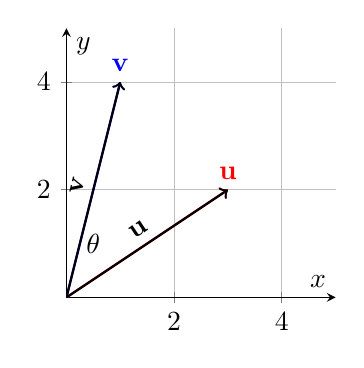
\begin{tikzpicture}
        \begin{axis}[
            axis lines = middle,
            xlabel = $x$,
            ylabel = $y$,
            xmin = 0, xmax = 5,
            ymin = 0, ymax = 5,
            width=5cm,
            height=5cm,
            grid=major,
            legend pos=north east,
            legend style={font=\small},
            axis equal image
        ]
        % Define the vectors
        \addplot[->, thick, red] coordinates {(0,0) (3,2)} node[above] {$\mathbf{u}$};
        \addplot[->, thick, blue] coordinates {(0,0) (1,4)} node[above] {$\mathbf{v}$};
        
        % Calculate the angle theta
        \draw[thick, ->] (axis cs: 0,0) -- (axis cs: 3,2) node[midway, above, sloped] {$\mathbf{u}$};
        \draw[thick, ->] (axis cs: 0,0) -- (axis cs: 1,4) node[midway, above, sloped] {$\mathbf{v}$};
        
        \node at (axis cs: .5, 1) {$\theta$};
        
        \end{axis}
    \end{tikzpicture}
\end{center}


\textbf{Proof:} Using polar coordinates, $u=\|u\|(\cos(\alpha), \sin(\alpha))$ and $v=\|v\|(\cos(\beta), \sin(\beta))$. Then \[
    \iprod{u,v} = \|u\|\|v\|(\cos(\alpha)\cos(\beta) + \sin(\alpha)\sin(\beta)) = \|u\|\|v\|\cos(\alpha-\beta)=\|u\|\|v\|\cos(\theta)
\]

\textbf{Definition:} $u\perp v$ if $\iprod{u,v}=0$

\textbf{Proposition:} $\|u+v\|^2 = \|u\|^2 + \|v\|^2 \iff u\perp v$, eg $\iprod{u,v}=0$

\textbf{Proof:} From the definition, \[
    \|u+v\|^2 = \iprod{u+v,u+v} = \iprod{u,u} + \iprod{v,v} + 2\iprod{u,v} = \|u\|^2 + \|v\|^2 + 2\iprod{u,v}
\]
which only matches iff. $\iprod{u,v}=0$.

\subsection{Cauchy Schwarz}
\textbf{Theorem (Cauchy Schwarz Inequality):} Let $u,v\in\rr^n$. Then \[
    |\iprod{u,v}| \leq \|u\|\|v\|
\]
\underline{Remark:} The proof works for any inner product satisfying the axioms, such as $\iprod{f,g}=\int_a^b f(x)g(x)dx$. (This is a HW Problem!)

\textbf{Proof:} Consider that if $\|u\|=0$ or $\|v\|=0$, then the inequality is trivially true. Thus, suppose that $\|u\|\neq 0$ and $\|v\|\neq 0$. Then, consider \[
    \|u-\alpha v\|^2
\]

The goal of this proof will be to minimize $\alpha$, and we will see that the Cauchy Schwarz Inequality just kind of drops out of it. We expand: \[
    0\leq\|u-\alpha v\|^2 = \|u\|^2 - 2\alpha\iprod{u,v} + \alpha^2\|v\|^2
\] 
Minimizing $-2\iprod{u,v}+2\alpha \|v\|^2=0$ gives us \[
    \alpha_0=\frac{\iprod{u,v}}{\|v\|^2}
\]
Substituting this back in, we get \begin{align*}
    0&\leq\|u\|^2 - 2\frac{\iprod{u,v}^2}{\|v\|^2}+\frac{\iprod{u,v}^2}{\|v\|^4}\|v\|^2 \\&= \|u\|^2 - \frac{\iprod{u,v}^2}{\|v\|^2}\\&= \frac{\|u\|^2\|v\|^2-\iprod{u,v}^2}{\|v\|^2}
\end{align*}

Thus, we have (by way of knowing that the denominator is $\geq 0$, and so the expression as a whole being $\geq 0$ requires the numerator to be as well)\[
    0\leq\|u\|^2\|v\|^2-\iprod{u,v}^2 \implies \iprod{u,v}^2\leq\|u\|^2\|v\|^2 \implies |\iprod{u,v}|\leq\|u\|\|v\|
\]
\qed 

\underline{Remark:} Equality in Cauchy Schwarz occurs iff. $u=\alpha v$ for some $\alpha\in\rr$.

One intuition is because the starting inequality we use in our proof is strict (by def of norm) unless $\|u-\alpha v\|=0$, which only occurs when $u-\alpha v=0$. Another way of thinking about it: Consider $u=\alpha v$. Then \[
    |\iprod{u,v}|=|\alpha|\|v\|^2=\|\alpha v\|\|v\| = \|u\|\|v\|
\]

Conversely, if $\|u\|\|v\|=\iprod{u,v}$, then the claim is that a vector is a scalar multiple of the other. We can see this by considering the proof of the Cauchy Schwarz Inequality, and see that the entire sequence of equalities on substitution works if and only if $\iprod{u,v}^2=0$ (on the last step). And thus going backwards, the norm of the vector $u-\alpha v$ is 0, which only occurs when $u=\alpha v$.

Another way of thinking about it: \[
    0\leq\|u-\alpha v\|^2 = \|u\|^2 - 2\alpha\iprod{u,v} + \alpha^2\|v\|^2
\]
This is a quadratic in $\alpha$, and the only way for this to be 0 is if the discriminant is 0, which is the case iff. $u=\alpha v$.

Prof. Machedon also mentioned the method to get this by noting $\|u-\alpha_0 v\|=0$ for $\alpha_0=\frac{\iprod{u,v}}{\|v\|^2}\implies u=\alpha_0 v$ by the second part of the 3rd axiom of vector spaces.

\textbf{Proposition (Triangle Inequality):} Let $u,v\in\rr^n$. Then \[
    \|u+v\|\leq\|u\|+\|v\|
\]
\textbf{Proof:} Since both values are non negative, it suffices to prove that the square of the left side is less than or equal to the square of the right. Squaring the left hand side, \begin{align*}
    \|u+v\|^2 &= \iprod{u+v,u+v} \\&= \|u\|^2 + \|v\|^2 + 2\iprod{u,v} \\&\leq \|u\|^2 + \|v\|^2 + 2\|u\|\|v\| \\&= (\|u\|+\|v\|)^2
\end{align*}

The $2\iprod{u,v}$ term is less than or equal to $2\|u\|\|v\|$ by the Cauchy Schwarz Inequality. \qed

\textbf{Proposition (Reverse Triangle Inequality):} Let $u,v\in\rr^n$. Then \[
    \|u\pm v\|\geq|\|u\|-\|v\||
\]

\textbf{Proof:} First, note that the case with $-$ implies the case with $+$ \& vice versa by just replacing $v$ with $-v$ (note that this doesn't change the norm operation on the right). Thus, we only need to prove the case with $-$.

Then we have \begin{align*}
    \|u\| &= \|u-v+v\|
    &\leq \|u-v\|+\|v\| &\text{(Triangle Inequality)}
\end{align*}
Rearranging, we get \[
    \|u\|-\|v\|\leq\|u-v\|
\]
\qed

\section{Limits}
Let $u$ be a limit point in $\rr^n$. Then let $\{u_k\}_{k\in \mathbb{N}}$ be a sequence in $\rr^n$ such that each $u_k$ is in $\rr^n$.

Just for this lecture, let the index be the superscript. For instance, $u_1=(u_1^1, u_1^2, \ldots, u_1^n), u_2=(u_2^1, u_2^2, \ldots, u_2^n), \ldots$

Thus $u^i=p^i u$ as notation. TODO: clarify this point. 

\subsection{Limit Definitions}
\textbf{Definition:} If $\{u_k\}$ is a sequence in $\rr^n$, and $u\in \rr^n$, then \begin{align*}
    \lim_{k\to\infty}u_k = u
\end{align*}
if $\lim_{k\to\infty}\|u_k-u\|=0$. i.e. \begin{align*}
    \fora \epsilon>0, \exists K\txt{s.t.}\|u_k-u\|<\epsilon\fora k\geq K.
\end{align*}

\textbf{Definition:} $\{u_k\}\to u$ (converges) componentwise if each $u_k^i\to u^i$ as $k\to\infty$.

\textbf{Proposition:} $\{u_k\}\to u$ in norm if and only if $\{u_k\}\to u$ componentwise.

\textbf{Proof:} Assume first $\{u_k\}\to u$ in norm. In other words, \begin{align*}
    \lim_{k\to\infty}\|u_k-u\|=0
\end{align*}
Then, for each fixed $1\leq i\leq n$, \begin{align*}
    |u_k^i-u^i|&\leq\sqrt{|u_k^1-u^1|^2+|u_k^2-u^2|^2+\ldots+|u_k^n-u^n|^2} \\&= \|u_k-u\|\to 0\txt{by assumption}
\end{align*}
By the comparison principle, each $\{u_k^i\}\to u^i$ as $k\to\infty$. Conversely, if each $\{u_k^i\}\to u^i$, then \begin{align*}
    \|u_k-u\|&=\sqrt{|u_k^1-u^1|^2+|u_k^2-u^2|^2+\ldots+|u_k^n-u^n|^2}
\end{align*}
We see that each part of this sum goes to 0, and thus the sum goes to 0. (by Math 410).\qed

\underline{Remark:} This only applies to finite $n$ dimensions. For infinite dimensions, this is not true. Let's take a look at that;

Let us look at $(\mathit{L}^2)=\{u^1, u^2, \dots\}$ with \begin{align*}
    \|u\|&=(\sum_{i=1}^{\infty}(u^i)^2)^{1/2}<\infty
\end{align*}
Then take a negative $\{u_k\}\in \mathit{L}^2$. Then $\{u_k\}\to u$ component wise if each $u_k^i\to u^i$. But $\{u_k\}\to u$ in norm if and only if $\|u_k-u\|\to 0$. Here, $\{u_k\}\to u$ componentwise but not in norm.

Take $u_1=(1,0,0,\ldots), u_2=(0,1,0,\ldots), u_3=(0,0,1,\ldots), \ldots$. Fix an $i$. What is the limit $\lim_{k\to\infty}u_k^i$? It is 0. For all $i$ in fact! Thus, we have pointwise convergence. But the norm of $u_k$ is 1 for all $k$, and thus the norm of the limit is 1. Thus, we do not have convergence in norm.

\section{Point Set Topology}

\subsection{Ballz and Open Sets}
\textbf{Definition:} Let $r>0, u\in \rr^n$. Then the open ball of radius $r$ centered at $u$ is \[
    B_r(u)=\{v\in \rr^n:\|v-u\|<r\}
\]

\textbf{Definition:} Let $A\subseteq \rr^n$ be a set. Then $A$ is open if \begin{align*}
    \fora u\in A, \exists r>0\txt{s.t.}B_r(u)\subseteq A
\end{align*}

\underline{Note:} Reading math: $r$ depends on $u$, since the $\exists$ is inside the $\forall$. If you reversed this, eg $\exists r>0\forall u\in A$, then $r$ would be fixed for all $u$. This, by the way, is the definition of the whole space (then $A$ is all $\rr^n$).

\textbf{Proposition:} All open balls are open sets.

\textbf{Proof:} Let the open ball be defined as $B_r(u)$. We need to show that, for some $v\in B_r(u)$, there is some $\rho>0$ such that $B_\rho(v)\subseteq B_r(u)$.

Let us fix such a $v$. Then for this $v$, \[
    \|v-u\|<r
\]
by definition. Try $\rho=r-\|v-u\|$. Now we need to check that $B_\rho(v)\subseteq B_r(u)$. Let $w\in B_\rho(v)$. Then \begin{align*}
    \|v-w\|&<\rho \\&= r-\|v-u\|
\end{align*}
To show that $w\in B_r(u)$, look at $\|u-w\|$. By the triangle inequality, \begin{align*}
    \|u-w\|&\leq \|u-v\|+\|v-w\| \\\|u-w\|&< \|u-v\|+\rho \\&= \|u-v\|+r-\|v-u\| \\&= r
\end{align*}\qed

\subsection{Closed Sets}
\textbf{Definition:} A set $A\subseteq \rr^n$ is closed if the following is always true: \begin{align*}
    \text{If }\{u_k\}\subseteq A\txt{ and }\{u_k\}\to u\in \rr^n\txt{, then }u\in A
\end{align*}

\textbf{Definition:} The complement of a set $A\subseteq \rr^n$ is \[
    A^c={\rr^n}^{\setminus A}=\{u\in \rr^n:u\notin A\}
\]

\textbf{Theorem:} $A$ is open iff. $A^c$ is closed.

\textbf{Proof:} Since this is an iff. statement, we prove in both directions.

$\Leftarrow$ Assume first that $A$ is open. To show $A^c$ is closed, let $\{u_k\}\subseteq A^c$, and assume $\{u_k\}\to u\in \rr^n$. If $u\in A^c$, we are done. If $u\notin A^c$, eg $u\in A$, then since $A$ is open $\exists r>0$ such that $B_r(u)\subseteq A$. But then no $u_k$ can be in $B_r(u)$, since $u_k\in A^c$. Thus, $u\notin A$, and thus $u\in A^c$. Thus, $A^c$ is closed.

$\Rightarrow$ Assume now that $A^c$ is closed. To show that $A$ is open, pick $u\in A$. We want there to $\exists r>0$ such that $B_r(u)\subseteq A$. Assume the contrary. Thus $\fora r>0, B_r(u)$ contains points in $A^c$. Lets call those points $V$. Note that $V$ is dependent on $r$. Let $r=\frac{1}{k}$. Thus we have some $V_k$. We know that $V_k\in A^c$, and $\|V_k-u\|<\frac{1}{k}$. Thus, $V_k\to u$ as $k\to\infty$. But $A^c$ is closed, and thus $u\in A^c$. This is a contradiction, and thus $A$ is open. \qed

\underline{Remark:} The statement $A$ is open iff. it is not closed is not true. For instance, $\rr^n$ is both open and closed. An example of a set that is neither open nor closed is $[0,1)$.

\underline{Claim:} $\emptyset$ is both open and closed. Checking this, $\fora u\in \emptyset$, it's trivial that $B_r(u)\subseteq \emptyset$, since anything is vacuously true for points in the empty set. Thus it's open. If $\{u_k\}\to u$ in the empty set, then it's once again vacuously true that $u\in \emptyset$. Thus it's closed. 

Other sets that are both open and closed don't exist but the proof is not simple. $\rr^n$ is path connected (future content) $\rightarrow \rr^n$ connected, to be discussed later.

\subsection{Open Set Properties}

\textbf{Proposition:} If $\{V_s\}_{s\in S}$ is a (possibility infinite) family of open sets, then \begin{align*}
    \bigcup_{s\in S}V_s\txt{ is open}
\end{align*}

\textbf{Proof:} Let $u\in \bigcup_{s\in S}V_s$. Then $u\in V_{s_0}$ for some $s\in S$. Since $V_{s_0}$ is open, $\exists r>0$ such that $B_r(u)\subseteq V_{s_0}\subseteq\bigcup_{s\in S}V_s$. Thus, $\bigcup_{s\in S}V_s$ is open. \qed

\textbf{Proposition:} If $\{V_s\}_{s\in S}$ is a finite family of open sets, then \begin{align*}
    \bigcap_{s\in S}V_s\txt{ is open}
\end{align*}

\textbf{Proof:} Let $u\in \bigcap_{s\in S}V_s$. Then $u\in V_s$ for all $s\in S$. Since every $V_s$ is open, $\exists r_s>0$ such that $B_{r_s}(u)\subseteq V_s$. Let $r=\min\{r_s:s\in S\}$. Then $B_r(u)\subseteq V_s$ for all $s\in S$, and thus $B_r(u)\subseteq \bigcap_{s\in S}V_s$. Thus, $\bigcap_{s\in S}V_s$ is open. \qed

\underline{Note:} This only works for finite families because the intersection of infinitely many open sets is not necessarily open. For instance, take $V_k=B_{1/k}(0)$. Then $\bigcap_{k=1}^\infty V_k=\{0\}$, which is not open. 

\subsection{Closed Set Properties}

\textbf{Proposition:} Let $\{F_s\}_{s\in S}$ be a possibly infinite family of closed sets, then \begin{align*}
    \bigcap_{s\in S}F_s\txt{ is closed}
\end{align*}

\textbf{Proof:} We know that \begin{align*}
    (\bigcap_{s\in S}F_s)^c=\bigcup_{s\in S}F_s^c\txt{ is open by DeMorgan's formula}
\end{align*}
We also know that each $F_s^c$ is open, and thus the union of all of them is open. Thus, the complement of the intersection is open, and thus the intersection is closed. \qed

\textbf{Proof but done another way:} Let $\{u_k\}\subseteq \bigcap_{s\in S}F_s$ and $\{u_k\}\to u\in \rr^n$. Then $u_k\in F_s$ for all $s\in S$. Since each $F_s$ is closed, $u\in F_s$ for all $s\in S$. Thus, $u\in \bigcap_{s\in S}F_s$. Thus, $\bigcap_{s\in S}F_s$ is closed. \qed

\textbf{Proposition:} Let $\{F_s\}_{s\in S}$ be a finite family of closed sets, then \begin{align*}
    \bigcup_{s\in S}F_s\txt{ is closed}
\end{align*}

\textbf{Proof:} We know that \begin{align*}
    (\bigcup_{s\in S}F_s)^c=\bigcap_{s\in S}F_s^c\txt{ is open by DeMorgan's formula}
\end{align*}
We also know that each $F_s^c$ is open, and thus the intersection of all of them is open. Thus, the complement of the union is open, and thus the union is closed. \qed

\textbf{Proof but done another way:} Let $\{u_k\}\subseteq \bigcup_{s\in S}F_s$ and $\{u_k\}\to u\in \rr^n$. Note here that $\{u_k\}$ can be spread across multiple groups. However at least one $F_s$ contains infinitely many $u_k$. In other words there's some $F_s$ and a subsequence $\{u_{i_l}\}_{l\in \mathbb{N}}\to u$ contained in that $F_s$. Thus, $u\in F_s$ for some $s\in S$. Thus, $u\in \bigcup_{s\in S}F_s$. Thus, $\bigcup_{s\in S}F_s$ is closed. \qed

\textbf{Definition:} Let $A\subseteq \rr^n$. Look at \begin{align*}
    \{u\in \rr^n|\exists r>0\txt{s.t.} B_r(u)\subseteq A\}\subseteq A
\end{align*} 
This set is called the \textbf{interior} of $A$, denoted $A^\circ$.

\textbf{Definition:} Let $A\subseteq \rr^n$. Look at \begin{align*}
    \{u\in \rr^n|\exists r>0\txt{s.t.} B_r(u)\subseteq A^c\}\subseteq A^c
\end{align*}
This set is called the \textbf{exterior} of $A$, denoted $A^e$.

\textbf{Definition:} Let $A\subseteq \rr^n$. Look at \begin{align*}
    \{u\in \rr^n|\fora r>0 B_r(u)\txt{meets both}A\txt{and}A^c\}
\end{align*}
This set is called the \textbf{boundary} of $A$, denoted $\partial A$.

\section{Continuous Functions}

\textbf{Definition:} Let $F:A\subseteq \rr^n\to \rr^m$. Then $F$ is continuous at $u\in A$ if \begin{align*}
    \fora \{u_k\}\subseteq A \txt{for which} \{u_k\}\to u, \{F(u_k)\}\to F(u)
\end{align*}

\underline{Example:} Take function $f:\{1,2\}\cup [3,\infty)\to \rr$. It will be defined by \begin{align*}
    f(x)=\begin{cases}
        1 & \txt{if x=1} \\
        0 & \txt{if x=2} \\
        x & \txt{if}x\in[0,\infty)
    \end{cases}
\end{align*}

Is this set continuous at $x=1$? Yes, because all sequences in $A$ that converge to $1$ then $\{f(u_k)\}$ also converges to 1 since all $u_k=1$ for a sufficiently large k. Basically the idea is that since it's an isolated point, all sequences that converge to 1 must be 1 after a cetain point, and thus it would also converge to $f(1)$.

Let $\epsilon=\frac{1}{10}, \exists K \txt{s.t.} |u_k-1|<\frac{1}{10}\fora k\geq K$, but $\{u_k\}\subset\{1,2\}\cup[3,\infty)$, and thus $u_k=1\fora k\geq K$. Thus, $f(u_k)=1\fora k\geq K$.

\textbf{Proposition:} Let $f,g: A\subseteq \rr^n\to \rr$. If $f,g$ are continuous at $u\in A$, then 
\begin{itemize}
    \item $\alpha f+\beta g$ is continuous at $u$ for all $\alpha,\beta\in \rr$.
    \item $fg$ is continuous at $u$.
    \item if $g(u)\neq 0\fora u\in A$, then $\frac{f}{g}$ is continuous at $u$.
\end{itemize}

\textbf{Proof:}\begin{itemize}
    \item Let $\{u_k\}\to u$. Then $\{f(u_k)\}\to f(u)$ and $\{g(u_k)\}\to g(u)$. Thus, $\{\alpha f(u_k)+\beta g(u_k)\}\to \alpha f(u)+\beta g(u)$.
    \item Let $\{u_k\}\to u$. Then $\{f(u_k)\}\to f(u)$ and $\{g(u_k)\}\to g(u)$. Thus, $\{f(u_k)g(u_k)\}\to f(u)g(u)$.
    \item Let $\{u_k\}\to u$. Then $\{f(u_k)\}\to f(u)$ and $\{g(u_k)\}\to g(u)$. Since $g(u)\neq 0$, $\{g(u_k)\}\neq 0$ for sufficiently large $k$. Thus, $\{\frac{f(u_k)}{g(u_k)}\}\to \frac{f(u)}{g(u)}$
\end{itemize}
\qed

\textbf{Proposition:} Let $F,G$ such that $F:A\subseteq \rr^n\to B\subseteq \rr^n$ and $G:B\subseteq \rr^n\to \rr^k$. Then if $F$ is continuous at $u\in A$ and $G$ is continuous at $F(u)$, then $G\circ F$ is continuous at $u$.

\textbf{Proof:} Let $\{u_k\}\to u$. Then $\{F(u_k)\}\to F(u)$ and $\{G(F(u_k))\}\to G(F(u))$. Thus, $\{G(F(u_k))\}\to G(F(u))$. \qed

\textbf{Proposition:} Let $F:A\subseteq \rr^n\to \rr^m$. Then $F$ is continuous at $u\in A$ iff. $\fora \epsilon>0 \exists \delta>0$ such that \[
    \|u-v\|<\delta\implies \|F(u)-F(v)\|<\epsilon
\]

\textbf{Proof:} Assume $\epsilon-\delta$ definition. Let $\{u_k\}\to u$. We want that $\{F(u_k)\}\to F(u)$. Let $\epsilon>0$. We are trying to find a $K$ such that the distance of $F(u_k)$ to $F(u)$ is less than $\epsilon$ for all $k\geq K$. Then $\exists \delta>0$ such that $\|u_k-u\|<\delta\implies \|F(u_k)-F(u)\|<\epsilon$. Since $\{u_k\}\to u$, $\exists K$ such that $\|u_k-u\|<\delta\fora k\geq K$. 

Then, $\|F(u_k)-F(u)\|<\epsilon\fora k\geq K$. \qed 

Conversely, assume the sequence definition holds. Then, assume by contradiction that the $\epsilon-\delta$ definition does not hold. Then, \begin{align*}
    \exists \epsilon>0 \txt{s.t.} \fora \delta>0, \exists v\in A, \|u-v\|<\delta \txt{s.t.} \|F(u)-F(v)\|\geq\epsilon
\end{align*}

Then, take $\delta=\frac{1}{k}$, to get \begin{align*}
    \{v_k\}\subseteq A, \|u-v_k\|<\frac{1}{k},\txt{and}\|F(u)-F(v_k)\|\geq\epsilon
\end{align*}
Thus we found a $\{v_k\}\subseteq A$ such that $\{v_k\}\to u$ but $\{F(v_k)\}\not\to F(u)$. This is a contradiction, and thus the $\epsilon-\delta$ definition holds. \qed

\underline{Recall:} If $F:A\to \rr^m$, if $B\subseteq A$ then $F|_B:B\to \rr^m$ is the restriction of $F$ to $B$ (also writeable as $F(B)$). Let there be a set $C$ in $\rr^m$. Then $F^{-1}(C)=\{u\in A:F(u)\in C\}$.

\underline{Remark:} $\epsilon-\delta$ definition is equivalent to the idea that $\fora \epsilon, \exists \delta$ such that \begin{align*}
    F(B_\delta(u)\cap A)\subseteq B_\epsilon(F(u))
\end{align*}
intuitively this is saying that if you take a ball of the elements of A around $u$ and map it to $F$, then it will be contained in a ball around $F(u)$.

This is also equivalent to \begin{align*}
    B_\delta(u)\cap A \subseteq F^{-1}(B_\epsilon(F(u)))
\end{align*}

\textbf{Theorem:} Let $O$ be open in $\rr^n$. Then $F:O\to \rr^m$. Then $F$ is continuous (eg continuous at every point) on $O$ iff. \begin{align*}
    F^{-1}(V)\txt{ is open in }O\txt{ for all open }V\subseteq \rr^m
\end{align*}

\textbf{Proof:} Assume $F^{-1}$ is open for all open $V\subseteq \rr^m$. Fix a $u$. We want to show that $\fora \epsilon>0, \exists \delta>0$ such that \begin{align*}
    B_\delta(u)\cap O \subseteq F^{-1}(B_\epsilon(F(u)))
\end{align*}

We need to pick a V. An obvious V to pick is $B_\epsilon(F(u))$. Then $F^{-1}(B_\epsilon(F(u)))$ is open by assumption. Thus $u\in F^{-1}(B_\epsilon(F(u)))$. Thus, $\exists \delta>0$ such that $B_\delta(u)\subseteq F^{-1}(B_\epsilon(F(u)))$. Thus, $F$ is continuous at $u$. We did not use $O$ open, but $O=F^{-1}(\rr^m)$ is open, implied by the idea that $F^{-1}(B_\epsilon(F(u)))$ is open.

Conversely, assume $F$ is continuous at every $u\in O$. Let $V\subseteq \rr^m$ be open. We want to show that $F^{-1}(V)$ is open. 

Let $u\in F^{-1}(V)$. We want to show that $\exists r>0$ such that $B_r(u)\subseteq F^{-1}(V)$. We know that $F(u)\subseteq V$. Since $V$ is open, $\exists \epsilon>0$ such that $B_\epsilon(F(u))\subseteq V$. Since $F$ is continuous at $u$, $\exists \delta>0$ such that $B_\delta(u)\cap O\subseteq F^{-1}(B_\epsilon(F(u)))\subseteq F^{-1}(V)$. We need to thus get rid of the $O$ in the intersection.

Since $O$ is open, and $u\in O, \exists \delta_1>0\txt{s.t.}B_{\delta_1}(u)\subseteq O$. Then let $r=\text{min}(\delta,\delta_1)$. Then $B_r(u)\subseteq B_\delta(u)\cap O\subseteq F^{-1}(V)$ \qed

\textbf{Corollary:} Let $f:\rr^n\to \rr$. If $f$ is continous, then for a fixed $\alpha\in \rr$, one of \begin{align*}
    \{u\in \rr^n | f(u)<\alpha\},\{u\in \rr^n|f(u)>\alpha\}
\end{align*}
is open.

\underline{Remark:}\begin{align*}
    \{u\in \rr^n | f(u)\leq \alpha\}
\end{align*} is closed because its complement, \begin{align*}
    \{u\in \rr^n | f(u)>\alpha\}
\end{align*} is open. This is because $f$ is continuous, and thus the inverse image of an open set is open.

\section{Compact Sets}

\subsection{Sequential Compactness}

\textbf{Definition:} The set $K\subseteq \rr^n$ is \underline{sequentially compact} if $\fora \{u_\mathit{l}\}\subseteq K, \exists \{u_{\mathit{l}_m}\}\txt{and}u\in K\txt{s.t.}\{u_{\mathit{l}_m}\}\to u$.

\textbf{Definition:} The set $A\subseteq \rr^n$ is \underline{bounded} if $\exists M\txt{s.t.}\|u\|\leq M\fora u\in A$.

\textbf{Proposition:} If $K\subseteq \rr^n$ is sequentially compact, then $K$ is bounded.

\textbf{Proof:} We want to find $M>0\txt{s.t.} \|u\|\leq M \fora u\in K$. Assume by contradiction that $K$ is not bounded. Then $\fora M>0, \exists u\in K\txt{s.t.}\|u\|>M$. 

Specify $M=m\in \mathbb{N}$. Then we find some $u_m\in K\txt{s.t.} \|u_m\|>m$. 

Then, $\{u_m\}\subseteq K$, but there is no subsequence that converges to a point in $K$. This is a contradiction, and thus $K$ is bounded. \qed

\textbf{Proposition:} If $K\subseteq \rr^n$ is sequentially compact, then $K$ is closed.

\textbf{Proof:} Pick some $\{u_\mathit{l}\}\subseteq K$. Assume that $\{u_\mathit{l}\}\to u\in \rr^n$. We want some $u\in K$. Since $K$ is sequentially compact, $\exists \{u_{\mathit{l}_m}\}\to u\in K$. Thus, $K$ is closed. \qed

\underline{Note: I'm going to stop using italic l here because i cannot be asked to MIT macro every time.}

\underline{Recall:} If $\{x_l\}\subseteq \rr$, and $\{x_l\}$ is bounded, then $\exists \{x_{l_m}\}\to x\in \rr$

\textbf{Proposition:} If $\{u_l\}\subseteq \rr^n$, and $\{u_l\}$ is bounded, then $\exists \{u_{l_m}\}\to u\in \rr^n$ (eg. every bounded sequence has a convergent subsequence).

\textbf{Proof:} We will use induction. \begin{itemize}
    \item $n=1$, this is clearly true lol 
    \item Assume the IH. Then $\exists \{u_l\}\subseteq \rr^n$ that has a convergent subsequence. 
    \item Let $\{u_l\}\subseteq \rr^{n+1}$. Also, $\{u_l\}$ is bounded. We write that \begin{align*}
        u_l=(u_l^1,u_l^2)
    \end{align*}
    where $u_l^1$ is of ""dimension"" $n$ and $u_l^2$ is of dimension 1.
    \item By the IH $\exists \{u_{l_m}'\}\to u'\in \rr^n$. 
    \item Look at $\{u_{l_m}^{n+1}\}$, which is a bounded sequence. Then $\exists \{u_{l_{m_p}}^{n+1}\}\to (u',u^{n+1})\in \rr$.
\end{itemize}

\underline{Note:} What the fuck, I'm gonna have to look back at this or find it in the textbook lol

\textbf{Theorem:} $K\subseteq \rr^n$ is sequentially compact iff. $K$ is closed and bounded. 

\textbf{Proof:} We have already shown that if $K$ is sequentially compact then it's closed and bounded. Let $K$ be closed and bounded. 

Pick some $\{u_l\}\subseteq K$. Then $\{u_k\}$ is bounded since it lives inside a bounded set, and thus $\exists \{u_{l_m}\}\to u\in \rr^n$. Since $K$ is closed, $u\in K$ and we are done.\qed

\textbf{Proposition:} If $K$ is sequentially compact and $F:K\to \rr^n$ is continuous then $F(K)$ is sequentially compact.

\textbf{Proof:} Let $\{u_l\}\subseteq F(K)$. Then $\exists \{u_k\}\subseteq K\txt{s.t.}F(u_k)=v_k$. Then $\exists \{u_{k_l}\}\to u\in K$, and $\{F(u_{l_k})\}\to F(u)$ by F being continuous. \qed

\underline{Question:} If $C\subseteq \rr^n$ is closed, $F:C\to \rr^m$ is continuous, is $F(C)$ closed? No. Take for instance $\frac{1}{1+x}$.

\underline{Question:} If $B\subseteq \rr$ is bounded, and $f:B\to \rr$ is continuous, is $f(B)$ bounded? No. Take for instance $f(x)=\frac{1}{x}$, $B=(0,1)$. Ten $f(B)=(1,\infty)$ which is not bounded.

\underline{Question:} If $B\subseteq \rr$ is bounded and $f:\rr\to \rr$ is continuous, is $f(B)$ bounded? Yes, take a compact set $B\subseteq K$. $K$ can just be $[a,b]$ where $a,b$ are the bounds of $B$. Then $K$ is seq compact and $f(K)$ is bounded.

\textbf{Theorem:} Let $K$ be sequentially compact. Then $f:K\to \rr$ is continuous. Then $f$ attains its minimum and maximum on $K$.

\textbf{Proof:} We know that $f(K)$ is bounded, and that $\exists m=\inf_{u\in K}f(u)$ (infimum). We want to show that $\exists u\in K\txt{s.t.}f(u)=m$. We know that $\exists \{u_i\}\subseteq K, f(u_i)\to m$. Since $K$ is sequentially compact, $\exists \{u_{i_k}\}\to u\in K$. Since $f$ is continuous, $f(u_{i_k})\to f(u)$. Since $f(u_{i_k})\to m$, $f(u)=m$.\qed

\textbf{Theorem:} Let $A\subseteq \rr^n$ be such that any $f:A\to \rr$ attaining its minimum and maximum values. Then $A$ is sequentially compact. 

\textbf{Proof:} We want to show that $A$ Is bounded and closed.\begin{itemize}
    \item Bounded - Choose $f(x)=\|x\|$. We know that $\exists x_{\text{max}}\in A\txt{s.t.}f(x)\leq f(x_{\text{max}})\fora x\in A$.
    
    i.e. $0\leq \|x\|\leq \|x_{\text{max}}\|\fora x\in A$. Thus, $A$ is bounded.
    \item Closed - Let $\{u_i\}\in A,\{u_i\}\to u\in \rr^n$. We want $u\in A$. Let $f(x)=\|x-u\|$. We choose this function because we wanted a function which has $0$ as an infimum. We also see that $f(u_i)\to 0$. Thus, $\exists u_i\txt{s.t.}f(u_i)\leq f(u_i)\leq f(u_{\text{max}})$. Thus, $u\in A$.
\end{itemize}

\subsection{Uniform Continuity}

\textbf{Definition:} $F:A\to \rr^m$ is \underline{uniformly continuous} if $\fora \{u_i\},\{v_i\}\subseteq A$ if $\{\|u_i-v_i\|\}\to 0$, then $\{\|F(u_i)-F(v_i)\|\}\to 0$.

\underline{Remark:} $F$ uniformly continuous implies $F$ continuous. The converse is not true. For instance, $f(x)=x^2$ is continuous but not uniformly continuous. In general, not all continuous functions are uniformly continuous.

$x^2$ is continuous but not uniformly continuous. Let $u_i=i, v_i=\frac{1}{i}+i$. Then $\|u_i-v_i\|\to 0$ but $\|f(u_i)-f(v_i)\|\not\to 0$.

Not all continuous $f:(0,1)\to \mathbb{R}$ are uniformly continuous. Take for instance $u_i=\frac{1}{i},v_i=\frac{1}{i^2}$. Then $f=\frac{1}{x}$ is continuous but not uniformly continuous.

\underline{Recall:} $F:A\subseteq \rr^n\to \rr^m$ is uniformly continuous if $\fora \{u_i\},\{v_i\}\subseteq A$, with $\|u_i-v_i\|\to 0$, then $\|F(u_i)-F(v_i)\|\to 0$.

\textbf{Theorem:} Let $K\subseteq \rr^n$ be sequentially compact, and $F:K\to \rr^m$ be continuous. Then $F:K\to \rr^m$ is uniformly continuous.

\textbf{Proof:} Let $F:K\to \rr^m$ continuous. Then assume by contradiction that $F$ is not uniformly continuous, i.e. $\exists \{u_i\}, \{v_i\}\subseteq K$ such that $\|u_i-v_i\|\to 0$ but $\|F(u_i)-F(v_i)\|\not\to 0$.

This means that $\fora \epsilon>0,\exists I\txt{s.t.}\|F(u_i)-F(v_i)\|\geq \epsilon\fora i\geq I$. We find a subsequence $\{u_{i_j}\}$ with $\|F(u_{i_j})-F(v_{i_j})\|\geq \epsilon$. Since $K$ is sequentially compact, $\exists \{u_{i_{j_k}}\}\to u\in K$. Since $F$ is continuous, $F(u_{i_{j_k}})\to F(u)$. But this is a contradiction because $\|F(u_{i_{j_k}})-F(v_{i_{j_k}})\|\geq \epsilon$ for all $k$. \qed

\textbf{Theorem:} Let $F:A\to \rr^m$. Then the following are requivalent:\begin{enumerate}
    \item if $\{u_i\},\{v_i\}\subseteq A$ and $\{\|u_i-v_i\|\}\to 0$, then $\{\|F(u_i)-F(v_i)\|\}\to 0$.
    \item $\fora \epsilon>0\exists \delta>0\txt{s.t.}\|u-v\|<\delta\implies \|F(u)-F(v)\|<\epsilon$
\end{enumerate}

\textbf{Proof:} $2\to 1$: Assume 2. Let $\{u_i\},\{v_i\}\subseteq A,\|u_i-v_i\|\to 0$. We want to show that $\|F(u_i)-F(v_i)\|\to 0$. Let $\epsilon>0$. Then $\exists I\txt{s.t.}\|u_i-v_i\|<\delta\fora i\geq I$. Then $\|F(u_i)-F(v_i)\|<\epsilon\fora i\geq I$. 

$1\to 2$: Assume 1. Equivalently, if 2 is not true, then 1 cannot be true. Thus, assume 2 is not true. Then $\exists \epsilon>0\txt{s.t.}\fora \delta>0,\exists u,v\in A\txt{s.t.}\|u-v\|<\delta\txt{but}\|F(u)-F(v)\|\geq \epsilon$. 

Let $\delta=\frac{1}{k}$. Then $\exists u_k,v_k\in A\txt{s.t.}\|u_k-v_k\|<\frac{1}{k}\txt{but}\|F(u_k)-F(v_k)\|\geq \epsilon$. Then $\{u_k\},\{v_k\}\subseteq A$ and $\{\|u_k-v_k\|\}\to 0$ but $\{\|F(u_k)-F(v_k)\|\}\not\to 0$. \qed 

\subsection{Path Connected/Intervals}

\textbf{Definition:} $A$ is \underline{convex} if $\fora u,v\in A$, the line segment $tu+(1-t)u$ between $u$ and $v$ is in $A \fora 0\leq t\leq 1$.

\textbf{Definition:} $A\subseteq \rr^n$ is \underline{path connected} if $\fora u,v\in A$, there exists a continuous function $\gamma:[a,b]\to A$ such that $\gamma(a)=u,\gamma(b)=v$. Then $\gamma$ is called the parametrized path.

\textbf{Theorem:} If $A\subseteq \rr^n$ is path connected and $F:A\to\rr^m$ is continuous, then $F(A)$ is path connected.

\textbf{Proof:} Let $u,v\in F(A)$. We want to find a parametrized path from $u$ to $v$. Let $x,y\in A$ such that $F(x)=u,F(y)=v$. Since $A$ is path connected, $\exists \gamma:[a,b]\to A$ such that $\gamma(a)=x,\gamma(b)=y$. Then $F\circ \gamma:[a,b]\to F(A)$ is a parametrized path from $u$ to $v$. \qed

\subsection{Connectedness}

\textbf{Proposition:} $A\subseteq \rr$ is path connected iff. $A$ is an interval $I$.

\textbf{Proof:} Assume $A$ is an interval. Let $u,v\in A$. Then let $\gamma:[0,1]\to A$. Then $\gamma(t)=tu+(1-t)v$ is a parametrized path from $u$ to $v$. Thus $A$ is path connected.

Assume $A$ is path connected. Let $u,v\in A$. We will show that $[u,v]\in A$. We know that $\exists \gamma:[a,b]\to A$ such that $\gamma(a)=u,\gamma(b)=v$. Let $w\in [u,v]$. We want that $w\in A$. By the IVT, $\exists c\in [a,b]\txt{s.t.}\gamma(c)=w$. Thus, $w\in A$ (since $\gamma:[a,b]\to A$). \qed

\textbf{Definition:} $A$ has the intermediate value property (IVP) if $\fora f:A\to \rr$, continuous, then $f(A)$ is an interval.

\textbf{Definition} $A\subseteq \rr^n$ is \underline{not connected} if $\exists U,V$ open sets such that \begin{enumerate}
    \item $U\cap A\neq \emptyset, V\cap A\neq \emptyset$
    \item $(U\cap A)\cap(V\cap A)=\emptyset$
    \item $(U\cap A)\cup(V\cap A)=A$
\end{enumerate}
\underline{Remark:} $U\cap A$ is called relatively open. If $U,V$ satisfy 1,2,3, then $U,V$ are said to separate $A$.

\textbf{Theorem:} $A$ is connected iff. $A$ has the IVP ($\fora f:A\to \rr$ continuous, then $f(A)$ is an interval).

\textbf{Proof:} We will show that $A$ is not connected is equivalent to $A$ does not have the IVP ($\exists f:A\to \rr$, continuous, such that $f(A)$ is not an interval).

Assume that $A$ is not connected. Then let $U,V$ open separate $A$. Let \begin{align*}
    f(x)=\begin{cases}
        1 & \txt{if}x\in A\cap U \\ 
        0 & \txt{if}x\in A\cap V \\
    \end{cases}
\end{align*}
$f$ is defined $\fora x\in A$ because of 3. The value $f(x)$ is unique because of 2. $f(A)=\{0,1\}$ because of 1. To show that $f$ is continuous at some $x_0\in U\cap A$, we need to show that $\exists \delta>0$ such that $B_\delta(x_0)\subseteq U$ (which is true, since U is open). Then if $x\in A$ and $\|x-x_0\|<\delta$, then $f(x)=f(x_0)$. Then $|f(x)-f(x_0)|=0<\epsilon$. We have thus found $f:A\to \rr$ continuous, $f(A)$ not an interval.

Conversely, assume $A$ does not have the IVP. Then let $f:A\to \rr$ be continuous such that $f(A)$ is not an interval. Then $\exists c\in \rr$ such that $c\notin f(A),f(A)\cap (-\infty,c) \neq \emptyset, f(A)\cap (c,\infty)\neq \emptyset$.

To construct $U,V$ separating $A$, let \begin{align*}
    \tilde{U}=f^{-1}((-\infty,c)), \tilde{V}=f^{-1}((c,\infty))
\end{align*}
Then $\tilde{U},\tilde{V}$ are not the empty set, because of the property that $f(A)\cap (-\infty,c)\neq \emptyset$ and $f(A)\cap (c,\infty)\neq \emptyset$. Then $\tilde{U}\cup \tilde{V}=A$ because of the property that $c\notin f(A)$. To finish the proof, we will find $U,V$ open such that \begin{align*}
    \tilde{U}=U\cap A,\tilde{V}=V\cap A
\end{align*}
Let $x\in \tilde{U}$ Then $f(x)<c$. Since $f$ is continuous, $\exists r(x)>0$ such that $f(y)<c \fora y\in B_{r(x)}(x)\cap A$. Let $U=\bigcup_{x\in \tilde{U}}B_{r(x)}(x)$. Note that $\tilde{U}=U\cap A=\bigcup_{x\in \tilde{U}}(B_{r(x)}(x)\cap A)$. If $x\in \tilde{U}$, then $x\in B_{r(x)}(x)\cap A$. If $y\in B_{r(x)}(x)\cap A$, for some $x\in \tilde{U}$, then $y\in \tilde{U}$. Thus we are done \qed 

\underline{Consequences:}\begin{itemize}
    \item $A$ being path connected implies $A$ has IVP is equivalent to $A$ connected 
    \item $A$ connected does not imply path connected
\end{itemize}

\textbf{Corollary:} If $U\subseteq \rr^n$ is both open and closed, then $U=\rr^n$ or $U=\emptyset$.

\textbf{Proof:} $\rr^n$ is path connected implies $\rr^n$ is connected. Let $U$ be both open and closed. Let $V=U^c$. Then $V$ is also open and closed. Thus $U\cup V=\rr^n$. We have that $U\cap V=\emptyset, U\cup V=\rr^n$. Is it possible for both of them to not be the empty set? No, because $\rr^n$ is connected. Thus $U=\emptyset$ or $U=\rr^n$. \qed

\textbf{Definition:} $K\subseteq \rr^n$ is \underline{compact} if $\fora$ family of open sets $\{V_\alpha\}$, if $K\subseteq \bigcup_{\alpha}V_\alpha$, then $\exists \{V_{\alpha_i}\}$ finite such that $K\subseteq \bigcup_{i=1}^n V_{\alpha_i}$.

\textbf{Theorem:} $K$ compact iff. $K$ is closed and bounded. 

\textbf{Proposition 1:} $K$ compact implies $K$ bounded. 

\textbf{Proof:} Our goal is to contain $K$ in the union of a finite amount of sets. Let $V_\alpha=B_\alpha(0), \alpha>0$. Then $\exists \alpha_1<\alpha_2<\alpha_l$ such that $K\subseteq \bigcup_{i\in\alpha}V_{\alpha_i}=B_{\alpha_n}(0)$.

\textbf{Proposition 2:} $K$ compact implies $K$ closed. 

\textbf{Proof:} Let $K$ compact. Then let $\{u_k\}\in K, \{u_k\}\to u\in \rr^n$. We want to show that $u\in K$. Assume, by contradiction, that $u\notin K$. Let $V_{l}=\{x\in \rr^n|\|x-u\|>\frac{1}{l}\}$. Then $\bigcup_{l=1}^\infty V_l=\rr^n\setminus \{u\}$. Also, $K\subseteq \bigcup_{l=1}^\infty V_l, V_1\subseteq V_2\subseteq\dots$. Thus $\exists V_{l_0}\txt{s.t.}K\subseteq V_{l_0}=\{x\in\rr^n|\|x-u\|>\frac{1}{l_0}\}$. This is a contradiction because we don't have $\{u_k\}\to u$. Thus $u\in K$. \qed

\textbf{Proposition:} If $L$ is compact, and $K\subseteq L$, and $K$ is closed, then $K$ is compact. 

\textbf{Proof:} Let $V_\alpha$ be open sets, with $K\subseteq \bigcup_{\alpha}V_\alpha$. Then $L\subseteq \bigcup_{\alpha}V_\alpha\cup K^c$. If $x\in K,\txt{then}x\in \bigcup_{\alpha}V_\alpha$. If $x\notin K$, then $x\in K^c$. That's why we needed the $K^c$ in the statement earlier. 

Since $L$ is compact, \begin{align*}
    \exists V_{\alpha_1},\dots,V_{\alpha_n}\txt{s.t.}K\subseteq V_{\alpha_1}\cup\dots\cup V_{\alpha_n}\cup K^c
\end{align*}

We of course want to get rid of the $K^c$. But by definition nothing in $K$ is in $K^c$. Thus, we have that $K$ is compact. \qed

\textbf{Theorem:} If $K\subseteq \rr^n$ is closed and bounded, then $K$ is compact. 

\textbf{Proof:} Since $K$ is bounded, $K$ is contained in some closed cube in $\rr^n$. For simplicity, assume that $K\subseteq[0,1]\times[0,1]\dots\times[0,1]=C$. By the previous proposition, it suffices to show taht $C$ is compact. Let $\{V_\alpha\}$ be a family of open sets such that $C\subseteq \bigcup_{\alpha}V_\alpha$ eg. it is an open cover of $C$.

Assume by contradiction there does not exist $V_{\alpha_i}$ finite subcover ($K\subseteq V_{\alpha_1}\cup V_{\alpha_2}\cup\dots\cup V_{\alpha_n}$ never happens). 

Divide $C$ into $2^n$ cubes of the form $C_i=[\frac{j_1}{2},\frac{j_1+1}{2}]\times[\frac{j_2}{2},\frac{j_2+1}{2}]\dots\times[\frac{j_n}{2},\frac{j_n+1}{2}]$ where $j_i=0,1$. So then there exists a subcube WLOG $C_1$ that cannot be covered by a finite amount of $V_\alpha$. 

Continuing, we will eventually find some subcube $C_2$, then $C_3$, and so on. None of these $C_i$ can be covered by finitely many $V_\alpha$. By a generalization of the Nested Interval Theorem to $\rr^n$, $\exists x_0\in C$ such that $x_0\in C_i$ for all $i$. Thus, $x_0\in C$ cannot be covered by any finite amount of $V_\alpha$. This is a contradiction. Thus, $K$ is compact. \qed

\section{Metric Spaces}
\subsection{Blah}
\textbf{Definition:} A set $X$ and $d:X\times X\to \rr$ is a \underline{metric space} if \begin{enumerate}
    \item $d(u,v)=d(v,u)\fora u,v\in X$ (symmetry)
    \item $d(u,v)\geq 0$ and $d(u,v)=0\iff u=v$ (non-negativity)
    \item $d(u,v)\leq d(u,w)+d(w,v)$ (triangle inequality)
\end{enumerate}

\underline{Example:} $X=\rr^n,d(u,v)=\|u-v\|$ is a metric space.

\underline{Remark:} In general, if $V$ is a vector space, $\|\cdot\|$ is called a norm if\begin{enumerate}
    \item $\|u\|\geq 0$
    \item $\|u\|=0\iff u=0$
    \item $\|u+v\|\leq \|u\|+\|v\|$
    \item $|\alpha|\|u\|=\|\alpha u\|$
\end{enumerate}

\textbf{Proposition:} If $\|\cdot\|$ is a norm, on a vector space $V$, then $d(u,v)=\|u-v\|$ is a metric.

\textbf{Proof:} To do so we need to prove each property.\begin{enumerate}
    \item $d(u,v)=\|u-v\|=\|v-u\|=d(v,u)$ by property 4 of norms.
    \item $d(u,v)=\|u-v\|\geq 0$ by property 1 of norms. If $d(u,v)=0$, then $\|u-v\|=0\implies u=v$ by property 2 of norms.
    \item $d(u,v)=\|u-v\|\leq \|u-w\|+\|w-v\|=d(u,w)+d(w,v)$ by property 3 of norms.
\end{enumerate}

\subsection{Practice Problems Time}
\begin{itemize}
    \item Let $f:\rr\to\rr$ continuous. Prove that $G=\{(x,f(x))|x\in\rr\}$ is closed. 
    \begin{itemize}
        \item By definition, this means that if there's a sequence of points and it converges to something then it must be in $G$. Let $\{(x_n,f(x_n))\}\to (x,y)$. We want to show that $(x,y)\in G$. 
        
        $x_n\to x$ because $f$ is continuous, and also $f(x_n)\to f(x)$. Since $f$ is continuous, $y_n=f(x_n)\to f(x)$ because it's in $G$. Thus, $(x,y)=(x,f(x))\in G$.
    \end{itemize}
    \item Is the converse to this true? eg. if you have a function $f:\rr\to\rr$ such that $G=\{(x,f(x))|x\in\rr\}$ is closed, does it imply that $f$ is continuous?
    \begin{itemize}
        \item Traditional thoughts: Attempt to prove it first. We have that $\{x_k\}\to x$, we hope to show that $f(x_k)\to f(x)$. We know that $\{(x_k,f(x_k))\}\subseteq G$ is closed. Then if $\set{(x_k),f(x_k)}\to(x,y)$, then $f(x)=y$. 
        
        We know that $\set{x_k}\to x$. If $\exists y\txt{s.t.}\set{f(x_k)}\to y$, then $y=f(x)$, and thus $f$ is continuous.

        If there is a counterexample, it has the feature that $\{f(x_k)\}$ does not converge to a real number. An example of this is $f(x)=\begin{cases}
            1 & x\in \mathbb{Q} \\
            0 & x\notin \mathbb{Q}
        \end{cases}$ The $x$ can converge to a point, but the $f(x)$ does not converge to anything. Thus, the converse is not true.
        
        There's also $f(x)=\frac{1}{x}$
    \end{itemize}
    \item How about if the graph domain was limited to $[0,1]$?
    \begin{itemize}
        \item The answer is that this is true, but it's hard to prove right now.
    \end{itemize}
    \item Let $C\subseteq\rr^n$ be a set with the property that any $f:C\to \rr$ which is continuous has to be uniformly continuous. Then, prove or disprove: C is a bounded set. \textit{Hint:} $f(x)=x^2$ is not uniformly continuous if $n, n+\frac{1}{n}\in C\fora n$. Prove or disprove: C is closed.
    \begin{itemize}
        \item No; Let's try $C=\mathbb{N}$. Let $f:\mathbb{N}\to\rr$ be some arbitrary function. Then $f$ is continuous automatically. Suppose that we have $\|x-y\|<\frac{1}{2}$. Then $|f(x)-f(y)|<\epsilon$ is true, since the only way this is possible is for $x=y$. Thus, $C$ is not bounded.
        \item Yes: Let's try to prove that $C$ is closed. Let $\{x_k\}\subseteq C$ and $x_k\to x$. We want to show that $x\in C$. On the contrary let $x\notin C$. Try $f(x)=\frac{1}{x}$. Then $f$ is not uniformly continous. For instance, let $\epsilon=1$. Then does there $\exists \delta>0$ such that $\|x-y\|<\delta\implies |f(x)-f(y)|<\epsilon$? No, let $x=x_k,y=x_l$, chosen such that $\|x_k-x_0\|<\frac{\delta}{2},\|x_l-x_0\|<\frac{\delta}{2}$. Then $|f(x_k)-f(x_l)|\to \infty$. Thus, $C$ is not closed.
    \end{itemize}
\end{itemize}

\subsection{Metrics}

\textbf{Definition:} Let $\|\cdot\|$ be a norm on a vector space $V$. Then $d(u,v)=\|u-v\|$ is a metric on $V$. (we already went over this definition but ok)

\underline{Examples:} (in $\rr^2$) \begin{itemize}
    \item $\|x\|=\sqrt{x_1^2+x_2^2}$ is a norm. Then $d(x,y)=\|x-y\|=\sqrt{(x_1-y_1)^2+(x_2-y_2)^2}$ is a metric.
    \begin{itemize}
        \item Also, $B_1(0)=\{x\in \rr^2|\|x\|<1\}$ uses this metric.
    \end{itemize}
    \item $\|x\|_1=|x_1|+|x_2|$ is a norm. Then $d(x,y)=\|x-y\|=|x_1-y_1|+|x_2-y_2|$ is a metric.
    \begin{itemize}
        \item Let's convince ourselves this is a norm. Then 
        \item $\|x\|\geq 0, \|x\|=0\iff x=0$
        \item $\|\alpha x\|=|\alpha x_1|+|\alpha x_2|=|\alpha|(|x_1|+|x_2|)=|\alpha|\|x\|$
        \item $\|x+y\|=|x_1+y_1|+|x_2+y_2|\leq |x_1|+|y_1|+|x_2|+|y_2|=\|x\|+\|y\|$
    \end{itemize}
    \item $\|x\|_\infty=\text{max}(|x_1|,|x_2|)$ is a norm. Then $d(x,y)=\|x-y\|=\text{max}(|x_1-y_1|,|x_2-y_2|)$ is a metric.
    \begin{itemize}
        \item Let's convince ourselves this is a norm. Then
        \item $\|x\|\geq 0, \|x\|=0\iff x=0$
        \item $\|\alpha x\|=\text{max}(|\alpha x_1|,|\alpha x_2|)=|\alpha|\text{max}(|x_1|,|x_2|)=|\alpha|\|x\|$
        \item $\|x+y\|=\text{max}(|x_1+y_1|,|x_2+y_2|)\leq \text{max}(|x_1|+|y_1|,|x_2|+|y_2|)=\|x\|+\|y\|$
    \end{itemize}
\end{itemize}

\underline{Note:} $\|x\|_\infty\leq \|x\|_1\leq \|x\|$ Also, all norms are comparable. eg. They can all be bounded, a sequence converging under one norm will converge under another norm, etc.

\textbf{Definition:} $X=C([a,b],\rr)=\{f:[a,b]\to\rr|f\txt{continuous}\}$ is the set of continuous functions from $[a,b]$ to $\rr$. 

\underline{Example:} In $\infty$ dimensions:

Let $X=C([a,b],\rr)=\{f:[a,b]\to\rr,f\txt{continuous}\}$ where $C$ is the set of continuous functions.
\begin{itemize}
    \item Then $\|f\|=\|f\|_\infty=\text{max}_{x\in[a,b]}|f(x)|$ is a norm.
    \begin{itemize}
        \item $max_{x\in[a,b]}|f_1(x)+f_2(x)|\leq max_{x\in[a,b]}|f_1(x)|+max_{x\in[a,b]}|f_2(x)|=\|f_1\|+\|f_2\|$
    \end{itemize}
    \item $\|f\|_1=\int_a^b|f(x)|dx$ is a norm.
    \begin{itemize}
        \item $\int_a^b|f_1(x)+f_2(x)|dx\leq \int_a^b|f_1(x)|dx+\int_a^b|f_2(x)|dx=\|f_1\|+\|f_2\|$
        \item $\int_a^b|\alpha f(x)|dx=|\alpha|\int_a^b|f(x)|dx=|\alpha|\|f\|$
        \item $\int_a^b|f(x)|dx\geq 0, \int_a^b|f(x)|dx=0\iff f(x)=0$
    \end{itemize}
    \item $\|f\|_2=\sqrt{\int_a^b|f(x)|^2dx}$ is a norm.
    \begin{itemize}
        \item $\sqrt{\int_a^b|f_1(x)+f_2(x)|^2dx}\leq \sqrt{\int_a^b|f_1(x)|^2dx}+\sqrt{\int_a^b|f_2(x)|^2dx}=\|f_1\|+\|f_2\|$
        \item $\sqrt{\int_a^b|\alpha f(x)|^2dx}=\sqrt{\alpha^2\int_a^b|f(x)|^2dx}=\alpha\sqrt{\int_a^b|f(x)|^2dx}=\alpha\|f\|$
        \item $\sqrt{\int_a^b|f(x)|^2dx}\geq 0, \sqrt{\int_a^b|f(x)|^2dx}=0\iff f(x)=0$
    \end{itemize}
\end{itemize}

\underline{Remark:} If $Y$ is a metric space with metric $d$, then any subset $X\subseteq Y$ is also a metric space

\underline{Generalities:} \begin{itemize}
    \item if $X$ is a metric space, the ball $B_r(p)=\{q\in X|d(p,q)<r\}$
    \item $A$ in $X$ is open if $\fora p\in A,\exists r>0\txt{s.t.}B_r(p)\subseteq A$ 
\end{itemize}

\textbf{Definition:} $A\subseteq X$ is closed if $\fora \{p_k\}\subseteq A$, if $\{p_k\}\to p\in X$, then $p\in A$.

\underline{Remark:} If $X$ is a metric space, then $X$ is open and closed in $X$.

\underline{Example:} $X=[0,1)$ with $d(x,y)=|x-y|$ has $X$ open and closed in itself.

\underline{Remark:} $\{f_k\}\subseteq C([a,b],\rr), \{f_k\}\to f$ with respect to $d(f,g)=\text{max}_{x\in[a,b]}|f(x)-g(x)|$ implies that $f_k\to f$ uniformly.

Recall from 410 that uniformly means that $\fora \epsilon>0,\exists N\txt{s.t.}\|f_k-f\|<\epsilon\fora k\geq N$.

\textbf{Definition:} $\{p_k\}\subseteq X$ is \underline{Cauchy} (or is a Cauchy sequence) if \begin{align*}
    \fora \epsilon>0, \exists K\txt{s.t.}d(p_k,p_l)<\epsilon\fora k,l\geq K
\end{align*}

\textbf{Definition:} $X$ is \underline{complete} if \begin{align*}
    \fora \txt{Cauchy seq}\in X\exists p\in X\txt{s.t.}\{p_k\}\to p
\end{align*}

\underline{Example:} For instance, the uniformly remark earlier has complete.

\underline{Comparison:} Take \begin{align*}
    \int_{a}^{b}|f(x)|dx
\end{align*}
for $f\in C([a,b],\rr)$. Then take \begin{align*}
    \text{max}_{x\in[a,b]}|f(x)|
\end{align*}

There is one clear inequality here. This is that \begin{align*}
    \int_{a}^{b}|f(x)|dx\leq (b-a)\text{max}_{x\in[a,b]}|f(x)|
\end{align*}

Does there $\exists c>0$ such that \begin{align*}
    \text{max}_{x\in[a,b]}|f(x)|\leq c\int_{a}^{b}|f(x)|dx
\end{align*}

No, take a function over 0 to 1 that drops from 1 to 0 very quickly. Then the max is 1, but the integral is very small. Thus, this inequality does not hold.

\underline{Question:} For $C([0,1],\rr)$ with $d(f,g)=\int_{0}^{1}|f-g|$, is this complete? 

One of the axioms of the norm is that $\|f\|=0\implies f=0$. As a remark, if $f$ is continuous, that's true. If $f$ is a general Riemann integrable function, then the above may fail. For instance, take the function which is $0$ everywhere except for one place, where it is $1$. Then the integral is 0, but the function is not 0. So this is not complete.

Let $f_n(x)=x^n, f_n:[0,1]\to\rr$. Then $\{f_n\}$ will approach $0$ if $x\in[0,1)$, and $1$ if $x=1$. Then $f_n$ goes to $0$ with respect to $d_1(f_n,0)=\int_{0}^{1}|f_n-0|dx$. And $f_n$ is not cauchy with respect to $d(f,g)=\text{max}_{x\in[0,1]}|f(x)-g(x)|$.

Then, let \begin{align*}
    f_n(x)=\begin{cases}
        x^n & x\in[0,1] \\
        1 & x\in[1,2]
    \end{cases}
\end{align*} Then \begin{align*}
    \int_{0}^{2}|f_n(x)-f(x)|dx\to 0\txt{if}f(x)=\begin{cases}
        0 & x\in[0,1) \\
        1 & x\in[1,2]
    \end{cases}
\end{align*}
eg $\int_{0}^{1}|f_n(x)-0|dx\to 0, \int_{1}^{2}|f_n(x)-1|dx\to 0$

So $f_n\to f$ with respect to $d$, therefore it is Cauchy. But there $\not\exists g\in C$ such that $\int_{0}^{2}|f-g|dx=0$. Thus, this is not complete. This is why we have to give up the Riemann integral and move to the Lebesgue integral.

\underline{Exercise:} Let $f_n\in C([0,1],\rr)$, $f_n(x)=x^n$. Then $d(f,g)=\text{max}_{x\in[0,1]}|f(x)-g(x)|$. This is not Cauchy.

How about $x^n(1-x)$? Is this Cauchy? Eg. Does it converge uniformly to something? For $x$ strictly less than 1, it converges to 0, and if $x=1$, it's identically 0. Thus the candidate for a limit is $f(x)=0 \fora x\in[0,1]$.

The issue is: $\max_{x\in[0,1]}x^n(1-x)\to 0$. 

\underline{Exercise (12.1, \#4)} Let $f_k\in C([0,1],\rr), f_k(x)=\cos(\frac{x}{k})$. Show that this converges uniformly. 

It is sufficient to show that the maximum of the absolute value of the difference between the function and the limit candidate goes to 0. 

\section{Existence and Uniqueness for ODEs}

\subsection{Uh Oh.}

\textbf{Definition:} Let $X$ be a metric space, and $T:X\to X$ be a map. Then $T$ is \underline{lipschitz} if $\exists M>0$ s.t. $d(T(p),T(q))\leq M\cdot d(p,q)\fora p,q\in X$.

\textbf{Proposition:} If $f:\rr\to\rr$, differentiable, then $f$ is lipschitz with constant $M$ iff. \begin{align*}
    |f'(x)|\leq M\fora x\in \rr
\end{align*}

\textbf{Proof:} If $f$ is differentiable, and lipschitz with constant $M$, then \begin{align*}
    |f(x)-f(y)|\leq M|x-y|\fora x,y\in \rr\\
    f'(x)=\lim_{h\to 0}\frac{f(x+h)-f(x)}{h}
\end{align*}
We know that this limit exists, and thus \begin{align*}
    |f'(x)|=\lim_{h\to 0}|\frac{f(x+h)-f(x)}{h}|\leq M
\end{align*} by the definition of lipschitz and the limit.

Conversely, if \begin{align*}
    |f'(x)|\leq M\fora x\in \rr\\
\end{align*} we want \begin{align*}
    |f(x)-f(y)|\leq M|x-y|\fora x,y\in \rr
\end{align*}

By the MVT, $\exists c\in (x,y)$ such that \begin{align*}
    f(x)-f(y)=f'(c)(x-y)
\end{align*} Then \begin{align*}
    |f(x)-f(y)|=|f'(c)||x-y|\leq M|x-y|\\
    |f(x)-f(y)|\leq M|x-y|
\end{align*} \qed

\textbf{Definition:} Let $T:X\to X$ be a \underline{contraction} if $\exists 0\leq c<1$ such that $d(T(p),T(q))\leq c\cdot d(p,q)\fora p,q\in X$. Basically, imagine a lipschitz function with $M<1$, and all the contraction does is "minimize" the function by a factor of $c$.

\textbf{Theorem:} big boy; Let $X$ be a complete (reminder, this means that all cauchy sequences converge) metric space, and $T:X\to X$ a contraction. Then this means $\exists$ unique $p\in X$ such that $T(p)=p$, called a \underline{fixed point}

\textbf{Proof:} \begin{itemize}
    \item Uniqueness: Suppose we have two fixed points, eg $T(p_1)=p_1, T(p_2)=p_2$. Then \begin{align*}
        d(p_1,p_2)=d(T(p_1),T(p_2))\leq c\cdot d(p_1,p_2)
    \end{align*} which is a contradiction unless $d(p_1,p_2)=0$. Thus, $p_1=p_2$.
    \item Existence: Pick any $p_0\in X, p_{k+1}=T(p_k)$. We know that for some $p_0,p_1,p_2,\dots$. We will show that $\{p_k\}$ is cauchy. Then \begin{align*}
        d(p_1,p_0)&\leq c\cdot d(p_1,p_0)\\
        d(p_1,p_2)&=d(T(p_0),T(p_1))\leq c\cdot d(p_0,p_1)\\
        d(p_2,p_3)&=d(T(p_1),T(p_2))\leq c\cdot d(p_1,p_2)\leq c^2\cdot d(p_0,p_1)\\
        &\vdots\\
        d(p_{k},p_{k+1})&\leq c^k\cdot d(p_0,p_1)
    \end{align*}
    Thus \begin{align*}
        d(p_{k},p_{k+l})&\leq d(p_{k+l},p_{k+l-1})+d(p_{k+l-1},p_k)\\
        &\leq d(p_{k+l},p_{k+l-1})+d(p_{k+l-1},p_{k+l-2})+\dots+d(p_{k+1},p_k)\\
        &\leq d(p_{k+l},p_{k+l-1})+\dots+d(p_{k+1},p_k)\\
        &\leq (c^{k+l-1}+c^{k+l-2}+\dots+c^{k})\cdot d(p_0,p_1)\\
        &\leq (c^k\sum_{l=0}^{\infty}c^l)d(p_0,p_1)\\
        &=c^k(\frac{1}{1-c})d(p_0,p_1)\\
        &\to 0\txt{uniformly as}k\to\infty
    \end{align*} 

    Now, let $\{p_k\}\to p$. We will show that $T(p)=p$. We must show that $T$ is continuous, i.e. if $p_k\to p$, then $T(p_k)\to T(p)$. Then \begin{align*}
        d(T(p_k),T(p))&\leq C\cdot d(p_k,p)\to 0\txt{basically, the lipschitz condition}\\
    \end{align*}

    And thus we have that $\{T(p_k)\}\to T(p)$. 

    We now know that $\{p_k\}\to p, \{T(p_k)\}\to T(p)$. Then $\{p_{k+1}\}\to T(p)$, and $\{p_{k+1}\}\to p$ by the uniqueness of limits. Thus, $T(p)=p$ \qed
\end{itemize}

\textbf{Set Up:} Suppose we have a set $O\subseteq \rr^2$, open. Then let us have a point $(x_0,y_0)\in O$. Let there be a function $g:O\to \rr$, continuous. Let $I$ be an interval, $f:I\to \rr$ such that the graph of $\{(x,f(x))|x\in I\}$ is contained in $O$.

\begin{figure}[H]
    \centering
    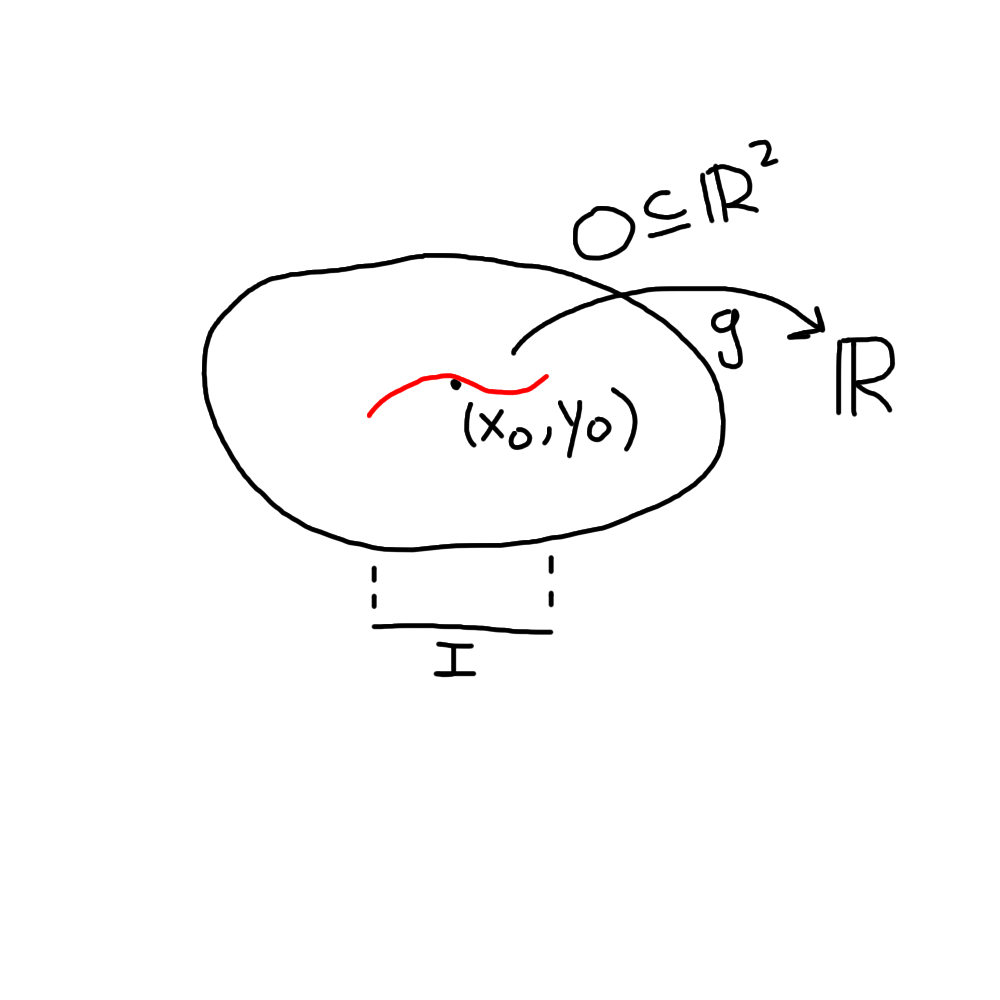
\includegraphics[height=5cm, trim=0 30px 0 30px, clip]{fig1.png}
    \caption{The setup (krita lol)}
    \label{fig:fig1}
\end{figure}

\textbf{The Existence Theorem:} Let $\mathcal{O}$ be an open subset of the plane $\rr^2$ that contains the point $(x_0,y_0)$. Suppose that the function $g:\mathcal{O}\to\rr^2$ is continuous and that there's a positive number $M$ such that \begin{align*}
    |g(x,y_1)-g(x,y_2)\leq M|y_1-y_2|\fora (x,y_1),(x,y_2)\in\mathcal{O}
\end{align*} Then, there exists a unique function $f:I\to\rr$ such that \begin{align*}
    \begin{cases}
        f'(x)=g(x,f(x))\fora x\in I \\
        f(x_0)=y_0
    \end{cases}
\end{align*}

\textbf{Proof:} For $\mathit{l}$, a positive number, define $I_\mathit{l}$ to be the closed interval $[x_0-\mathit{l},x_0+\mathit{l}]$. We will show that $\mathit{l}$ can be chosen such that there is exactly one continuous function $f:I_\mathit{l}\to\rr$ that satisfies \begin{align*}
    f(x)=y_0+\int_{x_0}^{x}g(s,f(s))ds\fora x\in I_\mathit{l}
\end{align*} Once such an $\mathit{l}$ is chosen, it follows from the Equivalence Lemma that there is exactly one solution of the differential equation on the interval $I=(x_0-\mathit{l},x_0+\mathit{l})$ that satisfies the initial condition $f(x_0)=y_0$.

Since $\mathcal{O}$ is open, we can choose positive numbers $a,b$ such that the rectangle $R=[x_0-a,x_0+a]\times[y_0-b,y_0+b]$ is contained in $\mathcal{O}$. Now for each positive number $\mathit{l}$ with $\mathit{l}\leq a$, define $X_\mathit{l}$ to be the subspace of the metric space $C(I_\mathit{l},\rr)$ consisting of the continuous functions $f:I_\mathit{l}\to \rr$ with the property that \begin{align*}
    |f(x)-y_0|\leq b\fora x\in I_\mathit{l}
\end{align*} Observe that $X_\mathit{l}$ consists of the continuous functions $f:I_\mathit{l}\to\rr$ whose graphs are contained in the rectangle $R$. 

For a function $f\in X_\mathit{l}$, define $T(f)\in C(I_\mathit{l},\rr)$ by \begin{align*}
    T(f)(x)=y_0+\int_{x_0}^{x}g(t,f(t))dt\fora x\in I_\mathit{l}
\end{align*} Observe that a solution of the integral equation is simply a fixed point of the mapping $T:X_\mathit{l}\to C(I_\mathit{l},\rr)$.

Since $C(I_\mathit{l},\rr)$ is a complete metric space and $X_\mathit{l}$ is a closed subset of it, it follows from a Corollary that $X_\mathit{l}$ is also a complete metric space. Now we will show that if $\mathit{l}$ is chosen to be sufficiently small, then \begin{align*}
    T(X_\mathit{l})\subseteq X_\mathit{l}, T:X_\mathit{l}\to X_\mathit{l}\txt{is a contraction}
\end{align*} and from the Contraction Mapping Principle it will follow that there is a unique fixed point of $T$ in $X_\mathit{l}$, which is a solution of the integral equation. Choose some positive $K$ such that \begin{align*}
    |g(x,y)|\leq K\fora (x,y)\in R
\end{align*}, which is allowed by the EVT. If $f$ is a function in $X_\mathit{l}$ and the point $x$ belongs to $I_\mathit{l}$, then \begin{align*}
    |T(f)(x)-y_0|&=|\int_{x_0}^{x}g(t,f(t))dt|\\
    &\leq \mathit{l}\cdot K
\end{align*} and thus $T(X_\mathit{l})\subseteq X_\mathit{l}$ assuming that $\mathit{l}\cdot K \leq b$. Now observe that if $f_1,f_2\in X_\mathit{l},x\in I_\mathit{l}$, then \begin{align*}
    |T(f_1)(x)-T(f_2)(x)|&=|\int_{x_0}^{x}g(t,f_1(t))-g(t,f_2(t))dt|\\
    &\leq |\int_{x_0}^{x}M\cdot d(f_1(t),f_2(t))dt\\
    &\leq |x-x_0|\cdot M\cdot d(f_1,f_2)\\
    &\leq \mathit{l}\cdot M\cdot d(f_1,f_2)
\end{align*} and thus $T:X_\mathit{l}\to X_\mathit{l}$ is a contraction. It follows that there is a unique fixed point of $T$ in $X_\mathit{l}$, which is a solution of the integral equation. \qed

\textbf{Lemma:} Assuming this set up, TFAE:\begin{itemize}
    \item $f$ is differentiable and \begin{align*}
        \begin{cases}
            f'(x)=g(x,f(x))\fora x\in I \\
            f(x_0)=y_0
        \end{cases}
    \end{align*}
    \item $f$ is continuous and $f(x)=y_0+\int_{x_0}^{x}g(t,f(t))dt$
\end{itemize}

\textbf{Proof:} Assume 1. Then $f\txt{diff}\implies f\txt{continuous}\implies f'\txt{continuous, since}f'(x)=g(x,f(x))$. Then \begin{align*}
    f(x)-y_0=f(x)-f(x_0)=\int_{x_0}^{x}f'(t)dt=\int_{x_0}^{x}g(t,f(t))dt
\end{align*}
which is 2. 

Assume 2. Since $f(x)=y_0+\int_{x_0}^{x}g(t,f(t))dt$, f is differentiable and $f'(x)=g(x,f(x))$. Also, $f(x_0)=y_0$ can be seen by taking $x=x_0$. Thus 1. \qed

\textbf{Theorem:} Assume, in addition, that $\exists M$ such that $|g(x,y_1)-g(x,y_2)|\leq M|y_1-y_2| \fora (x,y_1),(x,y_2)\in O$. Let $a,b>0$ s.t. \begin{align*}
    [x_0-a,x_0+a]\times[y_0-b,y_0+b]\subseteq O
\end{align*}
(imagine a box around the point in the illustration above). Then define, for $0<l\leq a$, \begin{align*}
    X_l=\{f:[x_0-l,x_0+l]\to[y_0-b,y_0+b]\}
\end{align*}
Then $\exists l>0$ such that $T(f)(x)=y_0+\int_{x_0}^{x}g(t,f(t))dt$ is a mapping $T:X_l\to X_l$, and is a contraction. Then $\exists! f\in X_l$ such that \begin{align*}
    f(x)&=y_0+\int_{x_0}^{x}g(t,f(t))dt\txt{,and}\\
    f'(x)&=g(x,f(x))\txt{,and}\\
    f(x_0)&=y_0
\end{align*}

\textbf{Proof:}\begin{align*}
    \exists K\txt{s.t.}|g(x,y)|\leq K\fora (x,y)\in[x_0-a,x_0+a]\times[y_0-b,y_0+b]
\end{align*}
We need to show that $T:X_l\to X_l$ if $l$ is sufficiently small. Consider $|T(f)(x)-y_0|$. Then \begin{align*}
    |T(f)(x)-y_0|&=|\int_{x_0}^{x}g(t,f(t))dt|\\
    &\leq |x-x_0|\cdot\text{max}_{t\in[x_0-l,x_0+l]}|g(t,f(t))|\\
    &\leq |x-x_0|\cdot K\\
    &\leq lK
\end{align*}

Thus if $l$ is really small, then $T(f)(x)\in [y_0-b,y_0+b]$. Thus $T:X_l\to X_l$.

Now we need to demonstrate that this is a contraction, provided that $l$ is sufficiently small. Then $\exists l>0$ such that \begin{align*}
    T(f)(x)=y_0+\int_{x_0}^{x}g(t,f(t))dt
\end{align*}
We want that \begin{align*}
    d(T(f_1),T(f_2))\leq c\cdot d(f_1,f_2)
\end{align*}
Then \begin{align*}
    |T(f_1)(x)-T(f_2)(x)|&\leq \int_{x_0}^{x}|g(t,f_1(t))-g(t,f_2(t))|dt\\
    &\leq \int_{x_0}^{x}M|f_1(t)-f_2(t)|dt\\
    &\leq M\cdot l\cdot\text{max}_{t\in[x_0-l,x_0+l]}|f_1(t)-f_2(t)|\\
    &=M\cdot l\cdot d(f_1,f_2)
\end{align*}
Then we get $d(T(f_1),T(f_2))\leq M\cdot l\cdot d(f_1,f_2)$. So as long as $M\cdot l<1$, then $T$ is a contraction.

Also, there thus $\exists! f:(x_0-l,x_0+l)\to [y_0-b,y_0+b]$ such that \begin{align*}
    f(x)&=y_0+\int_{x_0}^{x}g(t,f(t))dt\txt{,and}\\
    f'(x)&=g(x,f(x))\txt{,and}\\
    f(x_0)&=y_0
\end{align*} \qed

\underline{Note:} come back and review this;

\underline{Recall:} For a setup $B=[x_0-a,x_0+a]\times [y_0-b,y_0+b]$, $g:B\to \rr$ continuous, such that $\exists M$ such that \begin{align*}
    |g(x,y_1)-g(x,y_2)|\leq M|y_1-y_2|\fora (x,y_1),(x,y_2)\in B
\end{align*}

\textbf{Theorem:} If $g$ is as above, $\exists 0<l<a$ and \begin{align*}
    f:[x_0-l,x_0+l]\to [y_0-b,y_0+b]\txt{where b is such that}B=[x_0-a,x_0+a]\times[y_0-b,y_0+b]\subseteq O
\end{align*}, continuous, such that \begin{align*}
    f(x)=y_0+\int_{x_0}^{x}g(t,f(t))dt\fora |x-x_0|\leq l
\end{align*} and thus \begin{align*}
    f'(x)=g(x,f(x))\fora |x-x_0|\leq l,f(x_0)=y_0
\end{align*} In addition, if $f_1,f_2:[x_0-l,x_0+l]\to[y_0-b,y_0+b]$ are continuous, and satisfy the above conditions, then $f_1=f_2$.

If we drop the lipschitz condition, then we can't guarantee uniqueness.

\underline{Remark:} We can find an example of continuous $g$ for which uniqueness fails given no lipschitz condition. Take for instance take a function that's very close to 0, and then goes up after 0. \begin{align*}
    f(t)=\begin{cases}
        0 & \txt{if}t<0\\
        t^3 & \txt{if}t\geq 0
    \end{cases}
\end{align*}
Then, \begin{align*}
    f'(x)=\begin{cases}
        0 & \txt{if}x<0\\
        3x^2 & \txt{if}x\geq 0
    \end{cases}
\end{align*}
In other words $f(t)$ is a solution for the first order ODE $f'(t)=3f(t)^{2/3}$, and $f'(0)=0$. This is one solution. We claim this solution isn't unique. Another solution is $f(t)=0$ for all $t$.

In fact for the format \begin{align*}
    f(t)=\begin{cases}
        0 & \txt{if}t<0\\
        (t-c)^3 & \txt{if}t\geq 0
    \end{cases}
\end{align*} has infinitely many solutions. To demonstrate that this is not lipschitz, let's give that $g(t,y)=3y^{2/3}$, and $g$ is continuous. Then \begin{align*}
    |g(t,y_1)-g(t,y_2)|?M|y_1-y_2|
\end{align*} The derivative of the function is not bounded near 0, and thus the lipschitz condition fails, eg $\frac{\partial g}{\partial y}(t,y)$ is unbounded as $y\to 0$.

\underline{Remark:} Existence is a local property. As an example, \begin{align*}
    \begin{cases}
        f'(t)=f^2(t) \\
        f(0)=1
    \end{cases}
\end{align*} Then $f(t)=\frac{1}{1-t}$ is a solution for $(-\infty<t<1)$. But existence is not a global property. For instance, $f(t)=\frac{1}{1-t}$ is not necessarily a solution for $t\geq 1$.

\textbf{Theorem:} Let $g:\rr^2\to\rr$, and assume that \begin{align*}
    |g(t,y_1)-g(t,y_2)|\leq M|y_1-y_2|\fora (t,y_1),(t,y_2)\in \rr^2,M>0
\end{align*} If \begin{align*}
    f_1'(t)&=g(t,f_1(t)),f_1(t_0)=y_0\\
    f_2'(t)&=g(t,f_2(t)),f_2(t_0)=y_0 \fora t\in \rr
\end{align*} Then $f_1(t)=f_2(t)$ for all $t\in \rr$. We will show this two ways, one in a sort of diff-eq way and one in a topology way.

\textbf{Proof 1:} (The diff-eq proof) We will show that $f_1(t)=f_2(t)\fora t\geq t_0$. A similar proof will work for $t<t_0$. Consider the point \begin{align*}
    E(t)=(f_1(t)-f_2(t))^2
\end{align*} Machedon remarks he uses E because he thinks of it as energy

Then \begin{align*}
    E'(t)&=2(f_1(t)-f_2(t))(f'_1(t)-f'_2(t))\\ 
    &\leq 2|f_1(t)-f_2(t)||g(t,f_1(t))-g(t,f_2(t))|\\
    &\leq 2M|f_1(t)-f_2(t)||f_1(t)-f_2(t)|\\
    &=2ME(t)
\end{align*} Thus, $E'(t)\leq 2ME(t),E(t_0)=0$. Then $E'(t)-2ME(t)\leq 0$. Using an integrating factor, we will solve this; \begin{align*}
    \frac{d}{dt}(e^{-2Mt}E(t))&=e^{-2Mt}E'(t)-2Me^{-2Mt}E(t)\leq 0\\
\end{align*} We know that $E(t)e^{-2Mt}$ is decreasing, it is $0$ at $t_0$. We would like to conclude it's $0$. We know that $E(t)$ is positive, and also $e^{-2Mt}$ is positive. Thus $E(t)=0$ for all $t\geq t_0$. Thus $f_1(t)=f_2(t)$ for all $t\geq t_0$. A similar proof will work for $t<t_0$.\qed 

\textbf{Proof 2:} (The topology proof) Let $f_1,f_2:\rr\to\rr$ is differentiable. Then \begin{align*}
    f_1'(t)&=g(t,f_1(t)),f_1(t_0)=y_0\\
    f_2'(t)&=g(t,f_2(t)),f_2(t_0)=y_0 \fora t\in \rr
\end{align*}, etc, and also Lipschitz \begin{align*}
    |g(t,y_1)-g(t,y_2)|\leq M|y_1-y_2|\fora (t,y_1),(t,y_2)\in \rr^2,M>0
\end{align*} From our main theorem last time, we know that \begin{align*}
    \exists l>0\txt{s.t.}f_1(t)=f_2(t)\fora |t-t_0|\leq l
\end{align*} Consider the set \begin{align*}
    S=\{t|f_1(t)=f_2(t)\}
\end{align*} given that $f_1,f_2$ continuous. Then the set $S$ is closed. Let $t_1\in S$. Then $f_1(t_1)=f_2(t_1)$. We claim that $S$ is also open. Then, $\exists \delta>0$ such that $f_1(t)=f_2(t)\fora |t-t_1|<\delta$ because they satisfy the same diff'eq, and they take the same value. We claim that there's a neighborhood of this point where they are still the same. There's a theorem (local uniqueness theorem) applied to $t_1$ that says that there's a neighborhood of $t_1$ where the solution is unique. Thus, $S$ is open. Since $S$ is both open and closed, $S=\rr$ and thus $f_1=f_2$. (It's not empty because $t_0$) \qed

\subsection{Unnamed Topic} 

\underline{Remark:} In the metric space $C([0,1],\rr)$, with $\|f\|=\text{max}_{x\in[0,1]}|f(x)|$, closed and bounded sets need not be sequentially compact. As an example, take the closed unit ball $B=\{f\in C([0,1],\rr)|\|f\|\leq 1\}$, and $f_k(x)=x^k$ is a sequence in $B$. We claim that this sequence has no convergent subsequence.

This is because the limit of the sequence is not continuous. \begin{align*}
    f_k(x)\to \begin{cases}
        0 & x\in[0,1)\\
        1 & x=1
    \end{cases}
\end{align*} The limit of such a convergence subsequence would have to be continuous, and thus this sequence has no convergent subsequence.

\subsection{Reviewing Exam Problems}

\textbf{Problem 39a:} Let \begin{align*}
    X=\{f\in C([0,\pi],\rr), 1-\pi\leq f(x)\leq 1+\pi \fora x\in [0,\pi]\}\\
    T:X\to C([0,\pi],\rr), T(f)(x)=1+\int_{0}^{x}\cos(f(t))dt
\end{align*} Prove $T:X\to X$.

\textbf{Answer:} Let $f\in X$. We have to prove $1-\pi\leq T(f(x))\leq 1+\pi \fora x\in [0,\pi]$. Then \begin{align*}
    1-\pi\leq T(f(x))\leq 1+\pi\\
    1-\pi\leq 1+\int_{0}^{x}\cos(f(t))dt\leq 1+\pi\\
    -\pi\leq \int_{0}^{x}\cos(f(t))dt\leq \pi\\
\end{align*} i.e. we have to show that the integral is bounded by $\pi$. Then \begin{align*}
    |\int_{0}^{x}\cos(f(t))dt|\leq \int_{0}^{x}|\cos(f(t))|dt\leq \int_{0}^{x}1dt=x\leq \pi
\end{align*}

\textbf{Problem 39b:} Is $T$ a contraction?

\textbf{Answer:} Let $f_1,f_2\in X$. Then \begin{align*}
    (T(f_1)(x))=1+\int_{0}^{x}\cos(f_1(t))dt\\
    (T(f_2)(x))=1+\int_{0}^{x}\cos(f_2(t))dt
\end{align*} and the distance \begin{align*}
    d(T(f_1),T(f_2))&=\text{max}_{x\in[0,\pi]}|T(f_1)(x)-T(f_2)(x)|\\
    &=\text{max}_{x\in[0,\pi]}|\int_{0}^{x}\cos(f_1(t))-\cos(f_2(t))dt|\\
    &\leq \int_{0}^{\pi}|\cos(f_1(t))-\cos(f_2(t))|dt\\
    &\leq C\cdot d(f_1,f_2)
\end{align*} The inside of the last integral is equal by the MVT to $\sin(\theta(t))|f_1(t)-f_2(t)|$, and thus the integral is bounded by $\pi\cdot d(f_1,f_2)$. Thus, $T$ is a contraction. To elaborate the MVT; \begin{align*}
    g(x)-g(y)=g'(\theta)(x-y)
\end{align*} for some $\theta\in(x,y)$.

Try \begin{align*}
    f_1(t)=0\\
    f_2(t)=\pi
\end{align*} Then $d(f_1,f_2)=\pi$, and \begin{align*}
    T(f_1)=1+\int_{0}^{x}\cos(0)dt=1+x\\
    T(f_2)=1+\int_{0}^{x}\cos(\pi)dt=1-x\\
    d(T(f_1),T(f_2))=\text{max}_{x\in[0,\pi]}|1+x-(1-x)|=2\pi
\end{align*} So the Lipschitz constant is at least 2. For this specific $f_1,f_2$, $d(T(f_1),T(f_2))= 2\pi\cdot d(f_1,f_2)$. So it is not a contraction (not $<1$).

\textbf{Problem 39c:} If $f$ is a fixed point of $T$, what differential equation does $f$ satisfy?

\textbf{Answer:} \begin{align*}
    f(x)=1+\int_{0}^{x}\cos(f(t))dt\\
    f'(x)=\cos(f(x)),f(0)=1
\end{align*}
Does the solution to this exist for all $x\geq 0$? Then \begin{align*}
    g(x,y)=\cos(y), |g(x,y)|\leq K=1\\
    |g(x,y_1)-g(x,y_2)|\leq M|y_1-y_2|, M=1
\end{align*} Thus there exists $h=h(K,M)$ such that the solution to $f'(x)=\cos(f(x)),f(0)=1$ exists and is unique for $[x_0-h,x_0+h]$. Thus the solution exists for all $x\geq 0$ by just splitting it up into intervals of length $h$.

\underline{Remark:} Let $g:\rr^2\to\rr$, continuous, such that \begin{align*}
    \exists M,K\txt{with} |g(x,y)|\leq K\fora (x,y)\in \rr^2\\
    |g(x,y_1)-g(x,y_2)|\leq M|y_1-y_2|\fora (x,y_1),(x,y_2)\in \rr^2
\end{align*} Then the solution to $f'(x)=g(x,f(x)),f(x_0)=y_0$ exists and is unique for all $x\in \rr$. This works because the solution exists for $[x_0-h,x_0+h]$ for some $h$, and then we can just keep extending the interval - and $x_0$ is arbitrary (eg $K,M$ are independent of $x_0,y_0$).

\textbf{Problem 40a:} Let \begin{align*}
    X=\{f\in C([0,1],\rr), 0\leq f(x)\leq 1\fora x\in[0,1]\}\\
    (T(f))(x)=\int_{0}^{x}f(t)^{\frac{2}{3}}dt
\end{align*} Prove that $T:X\to X$.

\textbf{Answer:} If $0\leq f\leq 1$, then $0\leq f^{\frac{2}{3}}\leq 1$. Then \begin{align*}
    0\leq \int_{0}^{x}f(t)^{\frac{2}{3}}dt\leq \int_{0}^{x}1dt=x\leq 1
\end{align*} Thus $T:X\to X$.

\textbf{Problem 40b:} Is $T$ a contraction?

\textbf{Answer:} We expect $T$ not to be a contraction because the integral is not bounded by a constant. Let's try $f_1(t)=0,f_2(t)=1$. Then \begin{align*}
    T(f_1)(x)=0\\
    T(f_2)(x)=\int_{0}^{x}1dt=x
\end{align*} Then $d(T(f_1),T(f_2))=1\cdot d(f_1,f_2)$. Thus $T$ is not a contraction.

Is it the case that using a sufficiently small $f_2$ will make it a contraction? eg. does there exist $h>0$ such that $T:X\to X$ is a contraction?

Let \begin{align*}
    f_1(t)=0\\
    f_2(t)=\delta (\text{small})
\end{align*} Then $d(f_1,f_2)=\delta$. Then \begin{align*}
    T(f_1)(x)=0\\
    T(f_2)(x)=\int_{0}^{x}\delta^{\frac{2}{3}}dt=\delta^{\frac{2}{3}}x
\end{align*} Then $d(T(f_1),T(f_2))=h\cdot \delta^\frac{2}{3}$. Does there exist a $C$ such that that this is less than or equal to $C\cdot \delta$? No. 

\textbf{Problem something:} Let $X=\{f\in C([0,1],\rr),|f(x)|\leq 1\}$, and $T:X\to C([0,1],\rr)$ be \begin{align*}
    T(f)(x)=\int_{0}^{x}\cos(f(t))dt
\end{align*} Show that $T:X\to X$.

\textbf{Answer:} We check that \begin{align*}
    |\int_{0}^{x}\cos(f(t))dt|&\leq 1\fora x\in[0,1]\\
    &\leq \int_{0}^{1}|cos(f(t))|dt\leq 1
\end{align*} so $T:X\to X$.

\textbf{Problem something else:} Is $T$ a contraction?

\textbf{Answer:} \begin{align*}
    |T(f_1)(x)-T(f_2)(x)|&=|\int_{0}^{x}\cos(f_1(t))-\cos(f_2(t))dt|\\
    &? C\cdot \max_{t\in[0,1]}|f_1(t)-f_2(t)|\\
\end{align*} Is this true? Although moving abs val inside a definite integral is not always true, we can get away with it for this one \begin{align*}
    |\int_{0}^{x}\cos(f_1(t))-\cos(f_2(t))dt|&\leq \int_{0}^{1}|\cos(f_1(t))-\cos(f_2(t))|dt\\
    &=\int_{0}^{1}|\sin(\theta(t))||f_1(t)-f_2(t)|dt\txt{for some}\theta(t)\\
    &\leq \int_{0}^{1}|f_1(t)-f_2(t)|dt\\
\end{align*} However we missed finding a $c$ such that this is less than or equal to $c\cdot \max_{t\in[0,1]}|f_1(t)-f_2(t)|$. Thus this method doesn't work (since we found $c=1$). But it kind of does; let's continue \begin{align*}
    &\leq \sin(1)\cdot \max_{t\in[0,1]}|f_1(t)-f_2(t)|\\
\end{align*} and since $\sin(1)<1$, we have that $T$ is a contraction.

\textbf{Problem something else else:} Let $X=\{f\in C([0,\frac{1}{2}],,0\leq f(x)\leq 4)\}$, and $T:X\to C([0,\frac{1}{2}],\rr)$ be \begin{align*}
    T(f)(x)=1+\int_{0}^{x}f(t)dt
\end{align*} $T:X\to X$?

\textbf{Answer:} \begin{align*}
    0&\leq 1 \leq T(f)(x)\leq 1+\int_{0}^{x}f(t)dt\\
    &\leq 1+\int_{0}^{\frac{1}{2}}4dt\leq 3\leq 4
\end{align*} and thus $T:X\to X$.

\textbf{Problem something else else else:} Is $T$ a contraction? \begin{align*}
    |T(f_1)(x)-T(f_2)(x)|&=|\int_{0}^{x}f_1(t)-f_2(t)dt|\\
    &\leq \int_{0}^{\frac{1}{2}}|f_1(t)-f_2(t)|dt\\
    &\leq \frac{1}{2}\cdot \max_{t\in[0,\frac{1}{2}]}|f_1(t)-f_2(t)|\\
\end{align*} so $T$ is a contraction.

\textbf{Problem something else else else else:} Does it have a fixed point?

\textbf{Answer:} \begin{align*}
    f(x)=1+\int_{0}^{x}f(t)dt\implies f'(x)=f(x),f(0)=1
\end{align*} Thus $f(x)=e^x$ is a solution and is unique. Thus $T$ has a fixed point.

\textbf{Problem 1:} Let $f:\rr\to\rr$. Then $\exists \delta>0$ such that $|f(x)-f(y)|\leq \epsilon\fora |x-y|\leq \delta$. What does this mean? 

\textbf{Answer:} Well, it's uniformly continuous, but that's not the point; it means that $f$ is constant, since it implies $|f(x)-f(y)|=0$ for all $x,y$.

\textbf{Problem 2a:} \begin{align*}
    \max_{(x,y)\neq (0,0)}\frac{x+2y}{\sqrt{x^2+y^2}}=\max_{(x,y)\neq (0,0)}\frac{\iprod{(x,y),(1,2)}}{\|(x,y)\|}\leq \| (1,2)\|=\sqrt{5}
\end{align*} Then the maximizer of $(x,y)$ is $(1,2)$

\textbf{Problem 2b:} \begin{align*}
    \max_{(x,y)\neq (0,0)}\frac{x+y}{\sqrt{x^2+4y^2}}=\max_{(x,y)\neq (0,0)}\frac{\iprod{(x,2y),(1,\frac{1}{2})}}{\|(x,2y)\|}\leq \|(1,\frac{1}{2})\|=\sqrt{\frac{5}{4}}
\end{align*} Then the maximizer of $(x,y)$ is $(1,\frac{1}{4})$ since we want $(x,2y)=(1,\frac{1}{2})$.

\textbf{Problem 3:} $f:[1,\infty)\to\rr,f(x)=\frac{1}{x}$. Is this uniformly continuous? 

\textbf{Answer:} We need to find \begin{align*}
    |f(x_1)-f(x_2)|\leq 1\cdot|x_1-x_2|\fora x_1,x_2\in [1,\infty)?\\
    |f(x_1)-f(x_2)\leq |f'(\theta)||x_1-x_2|=\frac{1}{\theta^2}|x_1-x_2|\leq 1\cdot |x_1-x_2|
\end{align*} so $f$ is uniformly continuous.

\textbf{Problem 4:} Lemma: If $f:S\subseteq \rr\to\rr$ is uniformly continuous if it is lipschitz continuous on $S$.

\textbf{Answer:} We know that $\exists M\txt{s.t.}|f(x_1)-f(x_2)|\leq M\cdot|x_1-x_2|\fora x_1,x_2\in S$. Then we want to find \begin{align*}
    \fora \epsilon>0\exists \delta>0\txt{s.t.}|x_1-x_2|\leq \delta\implies |f(x_1)-f(x_2)|\leq \epsilon
\end{align*} Fix $\epsilon>0,\delta=\frac{\epsilon}{M}$ works. Then \begin{align*}
    |x_1-x_2|\leq \delta\implies |f(x_1)-f(x_2)|\leq M\cdot |x_1-x_2|\leq M\cdot \delta=\epsilon
\end{align*} and thus $f$ is uniformly continuous.

\textbf{Problem 5:} Let $f_k=x^k(1-x)^k, f_k\in C([0,1],\rr)$. Is $f_k$ Cauchy? Yes, it converges uniformly to 0.

\section{Differentiating Multivar Functions}

Chapter 13
\subsection{Limits}
\textbf{Definition:} $x_{*}$ is a limit point of $A\subseteq\rr^n$ if \begin{align*}
    \exists \{x_k\}\subseteq A\setminus \{x_{*}\}\txt{s.t.}\{x_k\}\to x_{*}
\end{align*}

\textbf{Definition:} If $f:A\to\rr$, and $x_{*}$ is a limit point of $A$, then \begin{align*}
    \lim_{x\to x_{*}}f(x)&=L\txt{if} \fora\{x_k\}\subseteq A\setminus\{x_{*}\},\\
    \lim_{k\to \infty}f(x_k)&=L
\end{align*}

Suppose \begin{align*}
    f(x,y)=\frac{xy}{x^2+y^2},f:\rr^2\setminus\{(0,0)\}
\end{align*}. Then the limit \begin{align*}
    \lim_{(x,y)\to (0,0)}f(x,y)\txt{DNE}
\end{align*}

To show this, consider $x_k=(\frac{1}{k},0)\to (0,0)$. Then $f(\frac{1}{k},0)=0\fora k$. So if the limit does exist, then it has to be 0. Take $x_k=(\frac{1}{k},\frac{1}{k})$. Then $f(\frac{1}{k},\frac{1}{k})=\frac{1}{2}\fora k$. Thus the limit does not exist.

\underline{Example:} Let \begin{align*}
    g(x,y)=\frac{x^2y}{x^2+y^2}
\end{align*} We claim that \begin{align*}
    \lim_{(x,y)\to (0,0)}g(x,y)=0
\end{align*}

Let $(x_k,y_k)$ be a sequence of points in $\rr^2$ that approach $(0,0)$. Then \begin{align*}
    |g(x_k,y_k)|&\leq |x_k|\frac{|x_ky_k|}{x_k^2+y_k^2}
\end{align*} The right half of the right side is bounded by $\frac{1}{2}$, and the left half goes to 0. Thus the limit is 0.

\textbf{Definition:} $f:\rr^n\setminus\{0\}\to \rr$ is homogeneous of degree $k$ if \begin{align*}
    f(tx)=t^kf(x)\fora t>0,x\in \rr^n\setminus\{0\}
\end{align*}

\underline{Remark:} What's special about $f,g$? According to the definition, $g$ is homogeneous of degree 1. $f$ is homogeneous of degree 0. Note that $g$ had a limit, and $f$ did not. Is this generalizable in some way?

\textbf{Proposition:} If $f:\rr^n\setminus\{0\}\to \rr$ is continous and homogeneous of degree $k>0$, then \begin{align*}
    \lim_{x\to 0}f(x)=0
\end{align*}

\textbf{Proof:} Let \begin{align*}
    f(x)&=f(\|x\|\cdot \frac{x}{\|x\|})\\
    &=\|x\|^kf(\frac{x}{\|x\|})
\end{align*} We try to bound the right side; consider the unit sphere, which is sequentially compact. We thus notice that $\frac{x}{\|x\|}\in S^{n-1}$, which is the $n-1$ dimensional sphere, and is seq. compact. We know that $f$ is continuous, so $f(\frac{x}{\|x\|})$ is bounded. Then for some $M$ \begin{align*}
    |f(x)|&=|\|x\|^kf(\frac{x}{\|x\|})|\\
    &\leq \|x\|^k\cdot M
\end{align*} Then $\lim_{x\to 0}f(x)=0$.

\underline{Remark:} What about functions homogeneous with degree $0$? We can't say anything about them. For instance, all constant functions are homogeneous of degree 0, and they can have a limit at 0. 

\subsection{Partial Derivatives}
\textbf{Definition:} Let $f:O\to \rr$, $x=(x_1,x_2,...,x_n)\in O\subseteq \rr^n, O$ open. Then \begin{align*}
    \frac{\partial f}{\partial x_i}(x)=\lim_{t\to 0}\frac{f(x+te_i)-f(x)}{t}
\end{align*}, if the limit exists. i.e. we keep all of the variables other than $x_i$ fixed, and then take $\frac{d}{dx_i}$.

\underline{Example:} Let $f:\rr^2\to\rr$, and \begin{align*}
    f(x,y)=\begin{cases}
        \frac{xy}{x^2+y^2} & (x,y)\neq (0,0)\\
        0 & (x,y)=(0,0)
    \end{cases}
\end{align*}
We notice that $f$ is not continuous at $(0,0)$. Note that $\frac{\partial f}{\partial x},\frac{\partial f}{\partial y}$ exist by the quotient rule at all $(x,y)\neq (0,0)$. As for the partial of $f$ wrt $x$ at 0, \begin{align*}
    \lim_{t\to 0}\frac{f(t,0)-f(0,0)}{t}=0
\end{align*}

\textbf{Definition:} If one $\frac{\partial f}{\partial x_i}(x)$ exists $\fora x\in O$, define \begin{align*}
    \frac{\partial f}{\partial x_i}(\frac{\partial f}{\partial x_j})=\frac{\partial^2 x}{\partial x_i x_j}
\end{align*}

\textbf{Theorem:} \* This is the theorem that says that if the partials exist and are continuous, then the order of differentiation doesn't matter. But I was mentally tapped out and didn't write it; I'll come back to it later. In the book, this is Thm 13.10 \*

\underline{Remark:} In general \begin{align*}
    \frac{d}{dt}|_{t=0}[f(x+th)]=\iprod{\nabla f(x),h}
\end{align*} where $\nabla f(x)$ is the gradient of $f$ at $x$.

\underline{Proposition:} Let $f:\rr^n\to\rr$, and assume that all $\frac{\partial f}{\partial x_i}(x)$ exists $\fora x\in \rr^n,\fora i\in \{1,\dots,n\}$. Fix $x, h\neq 0 (h\in \rr^n)$. Then $\exists z_1,\dots,z_n\in B_{\|h\|}(x)$ such that \begin{align*}
    f(x+h)-f(x)=\sum_{i=1}^{n}\frac{\partial f}{\partial x_i}(z_i)h_i
\end{align*}

\textbf{Proof:} Textbook has $n=3$. For us, let $n=2$. Then \begin{align*}
    f(x+h)-f(x)&=f(x_1+h_1,x_2+h_2)-f(x_1,x_2)\\
    &=f(x_1+h_1,x_2+h_2)-f(x_1,x_2+h_2)+f(x_1,x_2+h_2)-f(x_1,x_2)\\
    &=\frac{\partial f}{\partial x_1}(x_1+\theta_1 h_1,x_2+h_2)h_1+\frac{\partial f}{\partial x_2}(x_1,x_2+\theta_2 h_2)h_2\txt{for some}\theta_1,\theta_2\in (0,1)
\end{align*} by MVT. Then \begin{align*}
    f(x+h)-f(x)=\sum_{i=1}^{2}\frac{\partial f}{\partial x_i}(z_i)h_i
\end{align*} for some $z_1,z_2\in B_{\|h\|}(x)$.

\begin{figure}[H]
    \centering
    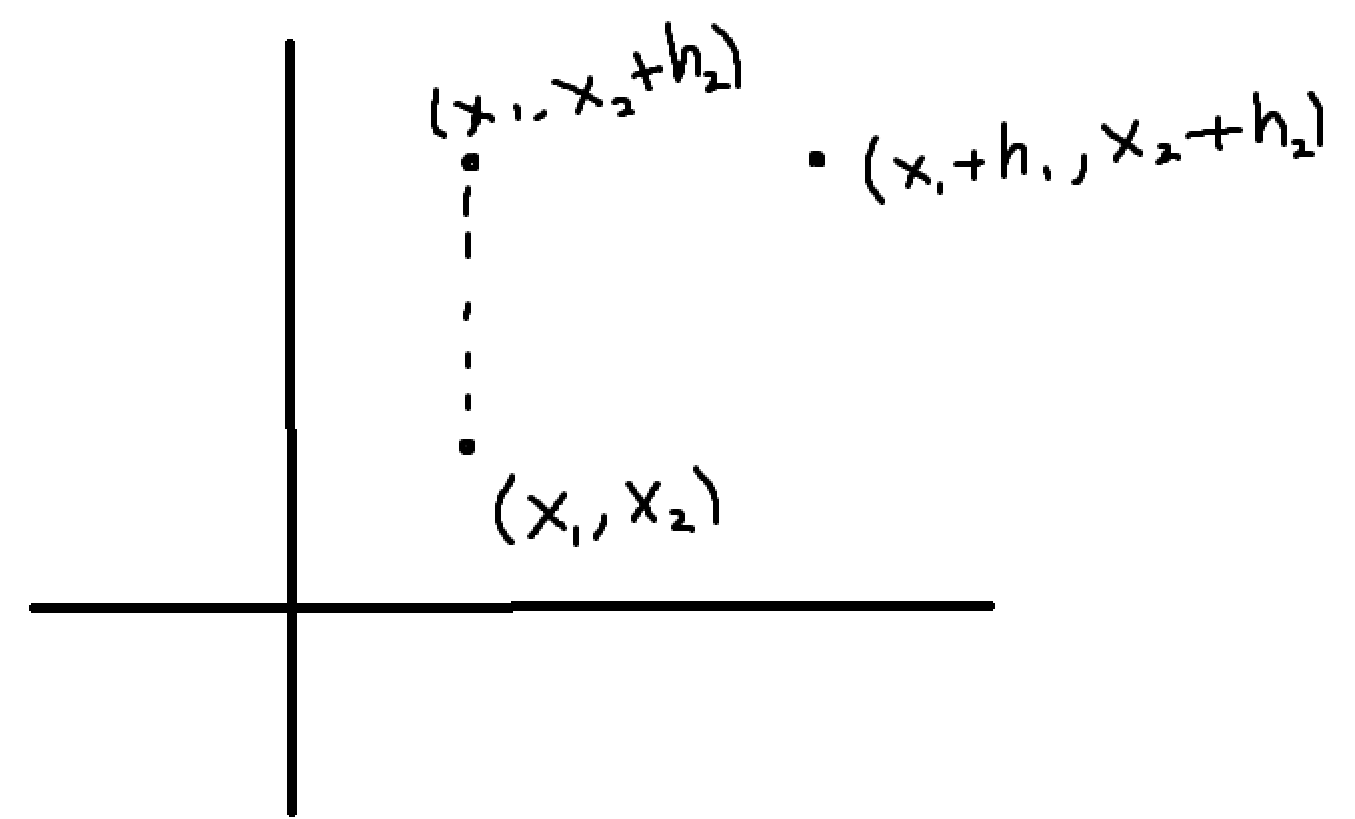
\includegraphics[height=5cm]{fig2.png}
    \caption{illustration}
    \label{fig:fig2}
\end{figure}

\textbf{Definition:} If $f:O\to \rr$, $O\subseteq \rr^n$ open, and all $\frac{\partial f}{\partial x_i}$ exist and are continuous, then $f$ is called continuously differentiable, or $C^1$.

\textbf{Theorem:} If $f:\rr^n\to\rr$ is $C^1$, then $\fora x\in \rr^n, h\neq 0$, the limit \begin{align*}
    \frac{d}{dt}|_{t=0}f(x+th)=\lim_{t\to 0} \frac{f(x+th)-f(x)}{t}=\sum_{i=1}^{n}\frac{\partial f}{\partial x_i}(x)h_i=\iprod{\nabla f(x),h}
\end{align*}

\textbf{Proof:} Consider $\frac{f(x+th)-f(x)}{t}$. By our previous proposition, this is \begin{align*}
    \frac{\sum_{i=1}^{n}\frac{\partial f}{\partial x_i}(z_i)t\cdot h_i}{t}
\end{align*} for some $z_1,\dots,z_n\in B_{t\|h\|}(x)$. Then as $t$ approaches 0 all of the $z_i$ approach $x$, and thus the limit is \begin{align*}
    \sum_{i=1}^{n}\frac{\partial f}{\partial x_i}(x)h_i
\end{align*} \qed

\subsection{Directional Derivative}

\textbf{Definition:} Let $p\neq 0, p\in \rr^n, f:\rr^n\to \rr$. The directional derivative of $f$ at $x$ in the direction of $p$ is \begin{align*}
    \frac{\partial f}{\partial p}(x)=\frac{d}{dt}|_{t=0}f(x+tp)\txt{if it exists}
\end{align*} and recall that \begin{align*}
    \nabla f(x)=(\frac{\partial f}{\partial x_1}(x),\dots,\frac{\partial f}{\partial x_n}(x))
\end{align*} and thus what we proved in the theorem immediately preceding this subsection is that if $f\in C^1$, then \begin{align*}
    \frac{\partial f}{\partial p}(x)=\iprod{\nabla f(x),p}
\end{align*}

\textbf{Theorem:} Let $f:\rr^n\to \rr$, $C^1$, $x\in \rr^n,h\in\rr^n,h\neq 0$. Then \begin{align*}
    \exists 0< \theta< 1\txt{s.t.} f(x+h)-f(x)=\iprod{\nabla f(x+\theta h),h}
\end{align*}

\textbf{Proof:} Let $\phi:\rr\to\rr,\phi(t)=f(x+th)$ so that $\phi(1)=f(x+h),\phi(0)=f(x)$. Then \begin{align*}
    f(x+h)-f(x)=\phi(1)-\phi(0)=\phi'(\theta)=\iprod{\nabla f(x+\theta h),h}
\end{align*}

\textbf{Theorem:} Let $f:\rr^n\to \rr$, and assume that all $\frac{\partial f}{\partial x_i}(x)$ exist and are continuous. Then $f$ is continuous. 

\textbf{Proof:} Consider $|f(x+h)-f(x)|$. By the previous theorem, this is \begin{align*}
    |\iprod{\nabla f(x+\theta h),h}|&\leq \|\nabla f(x+\theta h)\|\|h\|,\theta\in (0,1)\\
    &\to 0\txt{as} h\to 0
\end{align*} and thus $f$ is continuous.

\underline{Remark:} What's a slightly weaker condition than the partial derivatives being continuous that would still ensure continuity of $f$? We can say that $f$ is $C^1$ if all of the partial derivatives exist and are bounded.

You can see this in the latter half of the inequality; we just need $\|\nabla f(x+\theta h)\|$ to be bounded.

And if \begin{align*}
    f(x,y)=\begin{cases}
        \frac{xy}{x^2+y^2} & (x,y)\neq (0,0)\\
        0 & (x,y)=(0,0)
    \end{cases}
\end{align*} then \begin{align*}
    \frac{\partial f}{\partial x}(x,y)&=\frac{y(x^2+y^2)-xy(2x)}{(x^2+y^2)^2}\\
    &=\frac{y^3-x^2y}{(x^2+y^2)^2}
\end{align*} and \begin{align*}
    \frac{\partial f}{\partial y}(x,y)&=\frac{x(x^2+y^2)-xy(2y)}{(x^2+y^2)^2}\\
    &=\frac{x^3-xy^2}{(x^2+y^2)^2}
\end{align*} they are both homogeneous of degree $-1$, but are unbounded. 

\underline{Remark:} Let $f:\rr^n\to\rr, C^1$. Fix $x$ Then \begin{align*}
    \max_{\|p\|=1}\frac{\partial f}{\partial p}(x)
\end{align*} is attained for $p=\frac{\nabla f(x)}{\|\nabla f(x)\|}$.

\underline{Proof:} If $\|p\|=1$, then \begin{align*}
    \frac{\partial f}{\partial p}(x)&=\iprod{\nabla f(x),p}\\
    &\leq \|\nabla f(x)\|\|p\|\\
    &\leq\|\nabla f(x)\|
\end{align*} and thus the maximum would be $\|\nabla f(x)\|$. Now we show that this is attained if $p=\frac{\nabla f(x)}{\|\nabla f(x)\|}$. Then \begin{align*}
    \frac{\partial f}{\partial p}(x)&=\iprod{\nabla f(x),\frac{\nabla f(x)}{\|\nabla f(x)\|}}\\
    &=\|\nabla f(x)\|
\end{align*} \qed

\underline{Remark:} Let $f:\rr^n\to\rr, C^1$. Then \begin{align*}
    \lim_{h\to 0}\frac{f(x+h)-f(h)-\iprod{\nabla f(x),h}}{\|h\|}=0
\end{align*}

\underline{Proof:} The left hand side; \begin{align*}
    \frac{|\iprod{\nabla f(x+\theta h),h}-\iprod{\nabla f(x),h}|}{\|h\|}&=\frac{|\iprod{\nabla f(x+\theta h)-\nabla f(x),h}|}{\|h\|}\\
    &\leq \frac{\|\nabla f(x+\theta h)-\nabla f(x)\|\|h\|}{\|h\|}\to 0
\end{align*} We do this in order to define differentiable functions. 

\textbf{Definition:} For $f:\rr^n\to \rr$, $f$ is differentiable at $x$ if \begin{align*}
    \exists q\in \rr^n\txt{s.t.}\lim_{h\to 0}\frac{f(x+h)-f(x)-\iprod{q,h}}{\|h\|}=0
\end{align*} In $\rr$, this is the same as saying that the derivative exists, but in higher orders its even more powerful

Note that \begin{align*}
    f\in C^1\implies f\txt{diff}\implies \txt{all}\frac{\partial f}{\partial x_i}\txt{exist}
\end{align*} but none of the converses are true.

\underline{Recall:} If $f\in C^1(\rr^n)$, then \begin{align*}
    f(x+h)-f(x)=\iprod{\nabla f(x+\theta h),h}\txt{for some}0<\theta<1
\end{align*} and as a consequence we proved the above limit.

i.e. \begin{align*}
    f(x+h)=f(x)+\iprod{\nabla f(x),h}+E(x,h)=f(x)+\iprod{\nabla f(x),h}+o(\|h\|)
\end{align*} when \begin{align*}
    \lim_{h\to 0}\frac{E(x,h)}{\|h\|}=0\txt{or}\\
    f(y)=f(x)+\iprod{\nabla f(x),y-x}+o(\|y-x\|)
\end{align*} for $x$ fixed, $y$ close to $x$. This has a connection with the tangent plane to the graph of $f$ in two dimensions. 

Suppose $G=\{(y_1,y_2,f(y_1,y_2))\}$, and we would like to write down the tangent direction at a point $(x_1,x_2)$. Let there be a curve $\gamma_1(t)$. This is meant to be a parametrized curve. Suppose $\gamma_1(t)=(x_1+t,x_2,f(x_1+t,x_2))$. Then the first direction tangent $T_1=\gamma_1'(0)=(1,0,\frac{\partial f}{\partial x_1}(x_1,x_2))$.

Similarly let $\gamma_2(t)=(x_1,x_2+t,f(x_1,x_2+t))$. Then the second direction tangent $T_2=\gamma_2'(0)=(0,1,\frac{\partial f}{\partial x_2}(x_1,x_2))$.

Then we can let $N$, the normal vector, be $N=(-\frac{\partial f}{\partial x_1},-\frac{\partial f}{\partial x_2},1)$. Note that $N$ is orthogonal to $T_1,T_2$.

Then the tangent plane at $(x_1,x_2,f(x_1,x_2))$ is given by \begin{align*}
    \iprod{y_1,x_1,y_2-x_2,y_3-f(x_1x_2)} \cdot N = 0
\end{align*} Note that we are using $y$ to match the former notation. Continuing, we have that \begin{align*}
    y_3-f(x_1x_2)-\frac{\partial f}{\partial x_1}(x_1,x_2)(y_1-x_1)-\frac{\partial f}{\partial x_2}(x_1,x_2)(y_2-x_2)&=0,\txt{or}\\
    y_3=f(x_1,x_2)+\frac{\partial f}{\partial x_1}(x_1,x_2)(y_1-x_1)+\frac{\partial f}{\partial x_2}(x_1,x_2)(y_2-x_2)\\
    &=f(x_1,x_2)+\iprod{\nabla f(x_1,x_2),(y_1-x_1,y_2-x_2)}\\
\end{align*} which is the above in 2 dimensions. That is to say, we $f(y)$ is the tangent plane approximation to the graph of $f(y)$ at $(x_1,x_2,f(x_1,x_2))$.

\subsection{}

\textbf{Definition:} Let $A$ be an $n\times n$ symmetric matrix. Then, \begin{align*}
    A=\begin{bmatrix}
        a_{11} & a_{12} & \dots & a_{1n}\\
        a_{21} & a_{22} & \dots & a_{2n}\\
        \vdots & \vdots & \ddots & \vdots\\
        a_{n1} & a_{n2} & \dots & a_{nn}
    \end{bmatrix}
\end{align*} We define a quadratic form $Q$ by \begin{align*}
    Q(x)=\iprod{Ax,x}=\sum_{i=1}^{n}\sum_{j=1}^{n}a_{ij}x_ix_j
\end{align*}

The main application comes from \begin{align*}
    A=\nabla^2f(x)=\begin{bmatrix}
        \frac{\partial^2 f}{\partial x_1^2}(x) & \frac{\partial^2 f}{\partial x_1\partial x_2}(x) & \dots & \frac{\partial^2 f}{\partial x_1\partial x_n}(x)\\
        \frac{\partial^2 f}{\partial x_2\partial x_1}(x) & \frac{\partial^2 f}{\partial x_2^2}(x) & \dots & \frac{\partial^2 f}{\partial x_2\partial x_n}(x)\\
        \vdots & \vdots & \ddots & \vdots\\
        \frac{\partial^2 f}{\partial x_n\partial x_1}(x) & \frac{\partial^2 f}{\partial x_n\partial x_2}(x) & \dots & \frac{\partial^2 f}{\partial x_n^2}(x)
    \end{bmatrix}
\end{align*} for $f\in C^2$.  This is called the Hessian matrix.

\textbf{Proposition:} If $f\in C^2(\rr^n)$, and with $x,h$ fixed, then \begin{itemize}
    \item $\frac{d}{dt}f(x+th)=\iprod{\nabla f(x+th),h}=\sum_{i=1}^{n}\frac{\partial f}{\partial x_1}(x+th)h_i$
    \item $\frac{d^2}{dt^2}f(x+th)=\iprod{\nabla^2 f(x+th)h,h}=\sum_{i=1}^{n}\sum_{j=1}^{n}\frac{\partial^2 f}{\partial x_i\partial x_j}(x+th)h_ih_j$
    \item $\frac{d^3}{dt^3}f(x+th)=\sum_{i,j,k=0}^{n}\frac{\partial^3 f}{\partial x_i\partial x_j\partial x_k}(x+th)h_ih_jh_k$
\end{itemize}

\textbf{Proof:}\begin{itemize}
    \item For 1, we know from the previous section that \begin{align*}
        f(x+h)-f(x)=\iprod{\nabla f(x+\theta h),h}
    \end{align*} for some $\theta\in (0,1)$. Then \begin{align*}
        \frac{d}{dt}f(x+th)=\iprod{\nabla f(x+th),h}
    \end{align*}
    \item For 2, we build on 1; \begin{align*}
        \frac{d}{dt}[\frac{d}{dt}f(x+th)]&=\frac{d}{dt}[\sum_{i=1}^{n}(h_i\frac{\partial f}{\partial x_i}(x+th))]\\
        &=\sum_{i=1}^{n}\frac{d}{dt}[h_i\frac{\partial f}{\partial x_i}(x+th)]\\
        &=\sum_{i=1}^{n}\sum_{j=1}^{n}\frac{\partial f}{\partial x_i}\frac{\partial f}{\partial x_j}(x+th)h_ih_j
    \end{align*}
\end{itemize}

\textbf{Definition:} Let $A$ be an $n\times n$ symmetric matrix. Then $A=(a_{ij})$ is the notation for the matrix. Define \begin{align*}
    \|A\|=(\sum_{i=1}^{n}a_{ij}^2)^{\frac{1}{2}}
\end{align*}

\textbf{Proposition:} aka the Generalized Cauchy Schwarz Inequality. Let $A$ be an $n\times n$ symmetric matrix. Then \begin{align*}
    \|Ax\|\leq \|A\|\|x\|\fora h\in \rr^n
\end{align*}

\textbf{Proof:} We see that \begin{align*}
    Ax=\begin{bmatrix}
        a_{11} & a_{12} & \dots & a_{1n}\\
        a_{21} & a_{22} & \dots & a_{2n}\\
        \vdots & \vdots & \ddots & \vdots\\
        a_{n1} & a_{n2} & \dots & a_{nn}
    \end{bmatrix}\cdot \begin{bmatrix}
        x_1\\
        x_2\\
        \vdots\\
        x_n
    \end{bmatrix}=\begin{bmatrix}
        \sum_{j=1}^{n}a_{1j}x_j\\
        \sum_{j=1}^{n}a_{2j}x_j\\
        \vdots\\
        \sum_{j=1}^{n}a_{nj}x_j
    \end{bmatrix}
\end{align*}, and that \begin{align*}
    \|Ah\|^2&=(\iprod{\txt{row 1},h}^2+\iprod{\txt{row 2},h}^2+\dots+\iprod{\txt{row n},h}^2)\\
    &=\sum_{i=1}^{n}(\sum_{j=1}^{n}a_{ij}h_j)^2\\
    &\leq (\|a_{i1}\|^2+\|a_{i2}\|^2+\dots+\|a_{in}\|^2)(h_1^2+h_2^2+\dots+h_n^2)\\
    &=\sum_{i=1}^{n}(\|a_{i1}\|^2+\|a_{i2}\|^2+\dots+\|a_{in}\|^2)\|h\|^2\\
    &\leq (\sum_{i,j=1}^{n}\|a_{ij}\|^2)\|h\|^2\\
    &=\|A\|^2\|h\|^2
\end{align*} my transcription of this proof is dubious but the idea is there.

\textbf{Definition:} Suppose $A:\rr^n\to \rr^n$. Then \begin{align*}
    \|A\|_{op}=\sup_{\|x\|=1}\|Ax\|
\end{align*} This is the operator norm, which finds the maximum of the norm of the image of the unit sphere.

\underline{Remark:} The earlier norm definition is also denoted by $\|A\|_{HS}$ and means the Hilbert Schmidt norm. Note that \begin{align*}
    \|Ax\|\leq \|A\|_{HS}\\
    \|A\|_{op}\leq \|A\|_{HS}
\end{align*}

\textbf{Definition:} Let $A$ be a symmetric $n\times n$ matrix. Then $A$ is positive definite if $\iprod{Au,u}>0\fora u\neq 0$, and negative definite if $\iprod{Au,u}<0\fora u\neq 0$.

\underline{Lemma:} Let $A$ be a symmetric, positive definite matrix. Then \begin{align*}
    \exists c>0\txt{s.t.}\iprod{Au,u}\geq c\|u\|^2\fora u\in \rr^n
\end{align*}

\textbf{Proof:} Think of both sides and think about functions of $u$. They are both quadratic forms, and homogeneous of degree 2. Basically, \begin{align*}
    \iprod{Atu,tu}=t^2\iprod{Au,u}\\
    \|tu\|^2=t^2\|u\|^2
\end{align*}, $\fora t>0, \fora u\in \rr^n$. Since they are homogeneous of degree 2, it is thus sufficient to prove that this is true for $u$ on the unit sphere. Then, \begin{align*}
    \iprod{Au,u}=\iprod{A\frac{u}{\|u\|},\frac{u}{\|u\|}}\geq c
\end{align*} for some $c>0$. Basically, the first is true for $u$ iff. it is true for all $tu$, iff 1 is true for $\frac{u}{\|u\|}=\hat{u}$. 

Thus, it suffices to show that $\exists c>0$ s.t. $\iprod{A\hat{u},\hat{u}}\geq c$ for all $\hat{u}$ on the unit sphere. This is true because it's a continuous function on a compact set (the unit sphere), and thus attains a minimum.

The linear algebra proof would have been to diagonalize $A$ and then use the fact that the eigenvalues are positive. Then $c=\min\{\lambda_1,\dots,\lambda_n\}$.

\section{Exam Answers:}

\textbf{Problem 1a:} Suppose $f:(0,1)\to \rr$ is uniformly continuous. Write down the sequence definition of uniform continuity.

\textbf{Answer:} $\fora \{u_k\}, \{v_k\}\subseteq (0,1)$, if $\{\|u_k-v_k\|\}\to 0$, then $|f(u_k)-f(v_k)|\to 0$, or $\fora \epsilon>0, \exists \delta>0$ s.t. $|u-v|<\delta\implies |f(u)-f(v)|<\epsilon$.

\textbf{Problem 1b:} Negate the definition of uniform continuity.

\textbf{Answer:} $\exists \{u_k\}, \{v_k\}\subseteq (0,1)$ such that $\{\|u_k-v_k\|\}\to 0$ but $|f(u_k)-f(v_k)|\not\to 0$, or $\exists \epsilon>0$ s.t. $\fora \delta>0, \exists u,v$ with $|u-v|<\delta$ but $|f(u)-f(v)|\geq \epsilon$.

\textbf{Problem 1c:} Is $f(x)=\frac{1}{x}$ uniformly continuous on $(0,1)$?

\textbf{Answer:} No, because $f$ is not bounded on $(0,1)$. You can also use $u_k=\frac{1}{k},v_k=\frac{1}{k^2}$ and then show that the limit of the difference of functions is not 0.

\textbf{Problem 2:} The maximum value of \begin{align*}
    \frac{x_1-x_2+\dots+(-1)^{n+1}x_n}{\sqrt{x_1^2+\dots+x_n^2}}
\end{align*}

\textbf{Answer:} Recognize that this is a C-S problem. Then \begin{align*}
    \frac{\iprod{(x_1,\dots,x_n),(1,-1,1,\dots,\pm 1)}}{\|x\|}\leq \sqrt{n}
\end{align*} so the maximum is $\sqrt{n}$, and the maximizer is $(1,-1,1,\dots,\pm 1)$.

\textbf{Problem 3:} Let $\|u\|<1$. Then $\|u-v\|<1-\|u\|$. Prove that $\|u\|<1$

\textbf{Answer:} $\|v\|\leq \|v-u+u\|\leq \|v-u\|+\|u\|<1-\|u\|+\|u\|=1$.

\textbf{Problem 4a:} Let $f:\rr^n\to \rr$, continuous. Then prove that \begin{align*}
    \fora V\subseteq \rr^n,\txt{open},f^{-1}(V)\txt{open}
\end{align*}

\textbf{Answer:} Let $u\in f^{-1}(v)$. Then $f(u)\in V$. For $V$ open, $\exists \epsilon>0$ s.t. $B_{\epsilon}(f(u))\subseteq V$. Since $f$ is continuous, $\exists \delta>0$ s.t. $B_{\delta}(u)\subseteq f^{-1}(B_{\epsilon}(f(u)))\subseteq f^{-1}(V)$. Alternatively $\exists \delta>0$ s.t. $f_(B_{\delta}(u))\subseteq B_{\epsilon}(f(u))\subseteq V$. Thus $f^{-1}(V)$ is open.

\textbf{Problem 5a:} Let $l>0$. Then let \begin{align*}
    X_l=\{f:[0,l]\to [1,3]\}, \txt{continuous}
\end{align*} and let \begin{align*}
    T(f)(x)=1+\int_{0}^{x}f(t)^2dt
\end{align*} Show that $T:X_l\to X_l$.

\textbf{Answer:} We must show that if $f\in X_l$, then $T(f)\in X_l$. Then \begin{align*}
    1&\leq 1+\int_{0}^{x}f(t)^2dt\leq 3
\end{align*} The first part is clearly true, we need that \begin{align*}
    \int_{0}^{l}f(t)^2dt\leq 2\fora x\in [0,l]
\end{align*} An easy bound is to say that \begin{align*}
    \int_{0}^{l}f(t)^2dt\leq l*3^2=9l<2
\end{align*} so $l=\frac{2}{9}$.

\textbf{Problem 5b:} Find a sufficient condition on $l$ such that $T$ is a contraction. That is, find $l$ s.t. \begin{align*}
    \|T(f_1)-T(f_2)\|\leq c\|f_1-f_2\|
\end{align*}

\textbf{Answer:} Then \begin{align*}
    T(f_1)(x)-T(f_2)(x)&=\int_{0}^{x}f_1(t)^2-f_2(t)^2dt\\
\end{align*} We want the max of the absolute value of this to be less than or equal to the maximum distance between $f_1$ and $f_2$. Then \begin{align*}
    \text{max}_{x\in [0,l]}|T(f_1)-T(f_2)|&\leq \text{max}_{x\in [0,l]}\int_{0}^{x}|f_1(t)^2-f_2(t)^2|dt\\
    &\leq \int_{0}^{l}|f_1(t)+f_2(t)||f_1(t)-f_2(t)|dt\\
    &\leq \int_{0}^{l}6\cdot |f_1(t)-f_2(t)|dt\\
\end{align*} so $l\leq \frac{1}{6}$.

\textbf{Problem 6a:} Let $\{f_k\}$ such that $f_k:[-1,1]\to \rr$. Then let $f_k=(1+x)^k(1-x)^k$. Prove that \begin{align*}
    \{f_k\}\to 0\txt{uniformly}
\end{align*}

\textbf{Answer:} $(1+x)^k(1-x)^k=(1-x^2)^k\leq 1$. Note it goes to 1 if $x=0$. Otherwise it goes to 0.

\textbf{Problem 6b:} Is $f_k$ cauchy? 

\textbf{Answer:} No, because the limit is not continuous.

\section{Continuing Differentiating Multivar Functions}

\subsection{Second Order Approx Formula}

\underline{Recall:} If $f:\rr\to\rr$, $f''(x)$ exists for every $x$, then $\fora x,h\in \rr$, we have the following: \begin{align*}
    f(x+h)=f(x)+f'(x)h+\frac{1}{2}f''(x+\theta h)h^2\txt{for some}\theta\in (0,1)
\end{align*}

\textbf{Theorem:} Let $f:\rr^n\to \rr, C^2$, and let $x,h\in \rr^n$. Then \begin{align*}
    f(x+h)=f(x)+\iprod{\nabla f(x),h}+\frac{1}{2}\iprod{h,\nabla^2 f(x+\theta h)h}\txt{for some}\theta\in (0,1)
\end{align*}

\textbf{Proof:} Let $\phi(t)=f(x+th)$. Then $\phi(1)=\phi(0)+\phi'(0)+\frac{1}{2}\phi''(\theta)$ for some $\theta\in (0,1)$. Then notice that \begin{align*}
    \phi'(0)&=\frac{d}{dt}|_{t=0}f(x+th)=\iprod{\nabla f(x),h}\\
    \phi''(t)=\frac{d^2}{dt^2}f(x+th)&=\iprod{\nabla^2 f(x+th)h,h}
\end{align*}

\underline{Note:} This is basically Taylor's approximation for linear case with the remainder quadratic. We can expand this out to higher orders.

\textbf{Theorem:} Let $f:\rr^n\to \rr$, or from some open set in $\rr^n$, $C^2$. Then the limit \begin{align*}
    \lim_{h\to 0}\frac{f(x+h)-[f(x)+\iprod{\nabla f(x),h}+\frac{1}{2}\iprod{\nabla^2f(x)h,h}]}{\|h\|^2}=0
\end{align*} Let's call the quantity on the right in the numerator $A$. 

\textbf{Proof:} Then \begin{align*}
    \lim_{h\to 0}\frac{f(x+h)-A}{\|h\|^2}&=\lim_{h\to 0}\frac{f(x)+\iprod{\nabla f(x),h}+\frac{1}{2}\iprod{h,\nabla^2 f(x+\theta h)h}-A}{\|h\|}\\
    &=\lim_{h\to 0}\frac{\iprod{(\nabla^2f(x+\theta h)-\nabla^2f(x))h,h}}{\|h\|}\\
    &\leq \lim_{h\to 0}\frac{\frac{1}{2}\|(\nabla^2f(x+\theta h)-\nabla^2f(x))h\|\|h\|}{\|h\|^2}\txt{by the generalized C-S inequality}\\
    &\leq \lim_{h\to 0}\frac{\frac{1}{2}\|\nabla^2f(x+\theta h)-\nabla^2f(x)\|\|h\|^2}{\|h\|^2}\to 0\txt{as}h\to 0
\end{align*}

\underline{Recall:} $A$ being an $n\times m$ symmetric matrix is positive definite if $\iprod{Au,u}>0\fora u\neq 0$. Similarly for negative definite, if $\iprod{Au,u}<0\fora u\neq 0$.

Let $f:O \to \rr$, with $O$ open in $\rr$. Let $x\in O$. Then there is a strict local minimizer if \begin{align*}
    \exists \delta>0\txt{s.t.}f(x)< f(x+h)\fora 0\leq \|h\|<\delta
\end{align*} Also, $x$ is a strict local maximizer if \begin{align*}
    \exists \delta>0\txt{s.t.}f(x)> f(x+h)\fora 0\leq \|h\|<\delta
\end{align*} Revision: The $\leq$ should be $<$.

\textbf{Theorem:} For simplicity let $f:\rr^n\to \rr_I, C^2$. If $x$ is such that the gradient $\nabla f(x)=0$ and the Hessian $\nabla^2 f(x)$ is positive definite, then $x$ is a strict local minimizer.

\textbf{Proof:} We know that $f(x+h)=f(x)+\iprod{\nabla f(x),h}+\frac{1}{2}\iprod{\nabla^2 f(x)h,h}+R(h)$ where $R(h)$ is the remainder or error. But it's very small, such that \begin{align*}
    \lim_{h\to 0}\frac{R(h)}{\|h\|}\to 0
\end{align*} We are looking for a minimizer; we want to show that $f(x+h)>f(x)$ for $h$ small. First, it's clear that $\iprod{\nabla f(x),h}=0$. Then \begin{align*}
    f(x+h)-f(x)&=\frac{1}{2}\iprod{\nabla^2 f(x)h,h}+R(h)\\
    &\geq c\|h\|^2+R(h)\\
\end{align*} Since $\lim_{h\to 0}\frac{R(h)}{\|h\|}\to 0$, \begin{align*}
    \exists \delta>0\txt{s.t.}|R(h)<\frac{c}{2}\|h\|^2\fora \|h\|<\delta
\end{align*} i.e. $R(h)\geq -\frac{c}{2}\|h\|^2$ if $\|h\|<\delta$. Thus \begin{align*}
    f(x+h)-f(x)&\geq \frac{c}{2}\|h\|^2\fora \|h\|<\delta\\
    &>0\txt{if}0<\|h\|<\delta
\end{align*}Thus $x$ is a strict local minimizer. By a similar argument, if $\nabla^2 f(x)$ is negative definite, then $x$ is a strict local maximizer.\qed 

\underline{Remark:} What about the converse? Take $f:\rr^n\to \rr$, of class $C^2$. Assume $x$ is a strict local minimizer. Then $\nabla f(x)=0$. What about the hessian matrix? Does it have to be positive definite? No. An example where the strict local minimum is at 0 but the second derivative is not positive definite is $f(x)=x^4$.

\textbf{Definition:} If $f:\rr\to \rr, C^2$ has a minimizer at x, then $f'(x)=0, f''(x)\geq 0$. If $f''(x)\leq 0$, then $x$ is a strict local maximizer.

\textbf{Definition:} A matrix is positive semidefinite if $\iprod{Ax,x}\geq 0\fora x\in \rr^n$. Similarly, negative semidefinite if $\iprod{Ax,x}\leq 0\fora x\in \rr^n$.

\textbf{Theorem:} We will show that the converse of the above theorem is true. Let $f:\rr^n\to \rr, C^2$. If $\nabla f(x)=0$ and $\nabla^2 f(x)$ is positive semidefinite, then $x$ is a local minimizer.

\textbf{Proof:} Assume $f$ has a local minimizer at $x$. Look at $\phi(t)=f(x+th)$. Then $\phi\in C^2$, and $\phi$ has a maximizer at $t=0$. Then $\phi'(0)=0$ and $\phi''(0)\geq 0$. Then \begin{align*}
    \phi'(t)&=\iprod{\nabla f(x+th),h}\\
    \phi''(t)&=\iprod{\nabla^2 f(x+th)h,h}
\end{align*} Then $\phi'(0)=0$ implies that $\iprod{\nabla f(x),h}=0$. Then $\phi''(0)\geq 0$ implies that $\iprod{\nabla^2 f(x)h,h}\geq 0$. Thus $\nabla^2 f(x)$ is positive semidefinite.\qed

IN particular, if $f:\rr^n\to \rr, C^2$, then this has a local minimizer of $x$, then all the second derivatives of $f$ at $x$ are geq 0

If $f:\rr^n\to \rr, C^2$, and this has a local maximizer, then the second derivatives of $f$ at $x$ are less than or equal to 0

\textbf{Proposition:} Let $U$ be open in $\rr^n$, and $f:U\to \rr, C^2$, assume the laplacian \begin{align*}
    \Delta f(x)=\sum_{i=1}^{n}\frac{\partial^2 f}{\partial x_i^2}(x)>0 \fora x\in U
\end{align*} Then $f$ has no local maximizer in $U$.

\textbf{Proof:} Assume by contradiction, $x$ is an interior maximizer. Then $\nabla f(x)=0$ and $\nabla^2 f(x)\leq 0$. But then $\Delta f(x)\leq 0$, a contradiction. Thus $f$ has no local maximizer in $U$.\qed 


\underline{Note:} This is probably transcribed wrong at some point
\textbf{Theorem:} Let $U$ be a bounded open set, and $\bar{U}=U\cup \partial U$. where $\partial U$ is the bounded seq compact set $U$. Let $f\in C^2(U)$, $f$ continuous on $\bar{U}$, satisfying \begin{align*}
    \Delta f(x)\geq 0 \fora x\in U
\end{align*} Then \begin{align*}
    \max_{\bar{U}}f=\max_{\partial U}f
\end{align*}

\textbf{Proof:} First, it's obviously true that $\max_{\bar{U}}f\geq \max_{\partial U}f$ because the maximum on the boundary is a subset of the maximum on the closure. The interesting part is the reverse. Consider $f_\epsilon(x)=f(x)+\epsilon\|x\|^2$. Then the laplacian \begin{align*}
    \Delta f_\epsilon(x)=\Delta f(x)+2n\epsilon>0
\end{align*} Then $f_\epsilon$ has no local maximizer in $U$. \begin{align*}
    \max_{\bar{U}}f\leq \max_{\bar{U}}f_\epsilon\leq \max_{\partial U}(f+\epsilon\|x\|^2)\leq \max_{\partial U}f+\epsilon k, k=\max_{\partial U}\|x\|^2\\
\end{align*} Thus $\max_{\bar{U}}f\leq \max_{\partial U}f$. The same argument holds for the minimum.\qed

\underline{Remark:} Suppose \begin{align*}
    f(x,y)=\frac{x^2y}{x^2+y^2},\\
    \frac{\partial f}{\partial x}(0,0)=0
\end{align*} Is $f C^1$? i.e. are the partials both cont. at 0?

Using homogeneity, \begin{align*}
    f\txt{is}C^{\infty}\txt{in}\rr^n\setminus{(0,0)}
\end{align*} is homogeneous of degree 2. Then the derivatives are homogeneous of degree 1. Thus, if $f\in C^1(\rr^n\setminus{0})$ and is homogeneous of degree $k$, the derivatives are homogeneous of degree $k-1$

\begin{align*}
    \frac{\partial}{\partial x_i}[f(tx)]&=\frac{\partial}{\partial x_i}[t^kf(x)]
    t \frac{\partial f}{\partial x_i}(tx)&=t^k\frac{\partial f}{\partial x_i}(x)
\end{align*} 

\underline{Remark:} Let $x\in \rr^n$. Then let the multi index $\alpha=(\alpha_1,\dots,\alpha_n), a_i=\{0,1,\dots\}$

\textbf{Definition:} $|\alpha|=\alpha_1+\dots+\alpha_n$

\textbf{Definition:} $\alpha!=\alpha_1!\alpha_2!\dots\alpha_n!$

\textbf{Definition:} $x^\alpha=x_1^{\alpha_1}\cdot X_2^{\alpha_2}\dots$

\textbf{Definition:} $\partial^\alpha f(x)=(\frac{\partial^{|\alpha|}}{\partial x_1^{\alpha_1}\dots x_n^{\alpha_n}}f)(x)$

\textbf{Proposition:} \begin{align*}
    (x_1+\dots+x_n)^k=\sum_{|\alpha|=k}\frac{k!}{\alpha!}x^\alpha
\end{align*}, or the multinomial formula. 

\textbf{Proof:} For $n=2$, \begin{align*}
    (x_1+x_2)^k=\sum_{i=0}^{k}\frac{k!}{i!(k-i)!}x_1^ix_2^{k-i}
\end{align*} Let $\alpha=(i,k-i)$. Then $|\alpha|=k$ so this formula can be rewritten as \begin{align*}
    \sum_{|\alpha|=k}\frac{k!}{\alpha!}x^\alpha
\end{align*}

Now let the formula be true for $n-1$. Then \begin{align*}
    ((x_1+\dots+x_{n-1})+x_n)^k&=\sum_{i=0}^{k}\frac{k!}{i!(k-i)!}(x_1+\dots+x_{n-1})^ix_n^{k-i}\\
    &=\sum_{i=0}^{k}\frac{k!}{i!(k-i)!}[\sum_{|\beta|=i}\frac{i!}{\beta!}\tilde{x}^\beta]x_n^{k-i}\\
\end{align*} Define $\alpha=(\beta,k-i)$. We have that $|\beta=i|$ Thus the length $|\alpha|=k$. Thus $\frac{1}{(k-i)!\beta!}=\frac{1}{\alpha!}$ Also, $\tilde{x}^\beta x_n^{k-i}=x^\alpha$. So the sum total is \begin{align*}
    \sum_{|\alpha|=k}^{\frac{k!}{\alpha!}}x^\alpha
\end{align*} and we are done.

\underline{Remark:} Let $f\in C^k(\rr^n)$, and \begin{align*}
    f(x+h)=f(x)+\iprod{\nabla f(x),h}+\dots
\end{align*} Look at $\phi(t)=f(x+th), \phi:\rr\to\rr,C^1$. Then we know that \begin{align*}
    \phi(1)=\phi(0)+\phi'(0)+\frac{1}{2}\phi''(0)+\dots+\frac{1}{(k-1)!}\phi^{(k-1)}(0)+\frac{1}{k!}\phi^(k)(0)
\end{align*} This is the one dimensional taylor expansion, which we know from other places. We would like to express this differently; to express $\phi^{(k)}(t)$ in terms of the partial derivatives of $f$. 

The textbook has that \begin{align*}
    \phi'(t)&=\iprod{(\nabla f)(x+th),h}=(h\cdot\nabla)(x+th)=h_1\frac{\partial f}{\partial x_1}(x+th)+\dots+h_n(\frac{\partial f}{\partial x_n})(x+th)\\
    &=[(h_1\partial_1+\dots+h_n\partial_n)f](x+th)
\end{align*} and \begin{align*}
    \phi''(t)=\iprod{(\nabla^2 f)(x+th)h,h}=((h_1\partial_1+\dots+h_n\partial_n)^2 f)(x+th)\\
    \phi^(k)(t)=((h_1\partial_1+\dots+h_n\partial_n)^k f)(x+th)=\sum_{|\alpha|=k}\frac{k!}{\alpha!}(h^\alpha\partial^\alpha f)(x+th)
\end{align*}

\textbf{Theorem:} Let $f:\rr^n\to\rr, C^k$. Then \begin{align*}
    f(x+h)&=\sum_{0}^{k-1}\sum_{|\alpha|=j}\frac{1}{\alpha!}\partial^a f(x)h^\alpha+\sum_{|\alpha|=k}\frac{1}{\alpha!}\partial^\alpha f(x+\theta h)h^\alpha\\
    &=\sum_{|\alpha|\leq k-1}\frac{1}{\alpha!}\partial^af(x)h^\alpha+\sum_{|\alpha|=k}\frac{1}{\alpha!}\partial^\alpha f(x+\theta h)
\end{align*} Notice the similarity with the one dimensional taylor expansion, where \begin{align*}
    \phi(x+h)=\sum_{i=0}^{k-1}\frac{1}{i!}\phi^i(x)h^i+\frac{1}{k!}\phi^{(k)}(x+\theta h)h^k
\end{align*}

\section{Review of Lin Alg}

\textbf{Definition:} $T:\rr^n\to \rr^n$ is linear if $T(\alpha u+\beta v)=\alpha T(u)+\beta T(v)$

\textbf{Theorem:} If $T:rr^n\to\rr^n$ is linear, then $\exists! m\times n$ matrix $A$ such that $T(u)=Au\fora u\in \rr^n$

\textbf{Proof:} Also, uniqueness; if $T(u)=Au$ and $T(u)=Bu$, then $A=B$. You can show that $A$ is the matrix of $T$ by showing that $Ae_i=T(e_i)$.

Existence: Let $e_1,\dots,e_n$ be the standard basis in $\rr^n$. Let $u=(u_1,\dots,u_n)=u_1e_1+\dots+u_ne_n$. Then \begin{align*}
    T(n)&=T(u_1e_1+\dots+u_ne_n)=u_1T(e_1)+\dots+u_nT(e_n)\\
    &=(T(e_1),\dots,T(e_n))\begin{bmatrix}
        u_1\\
        \vdots\\
        u_n
    \end{bmatrix}
\end{align*} Thus $A=(T(e_1),\dots,T(e_n))$.

\textbf{Proposition:} Let $\rr^n\to^T_A\rr^m\to^S_B\rr^k$, where $T,S$ are linear transforms. Let $A,B$ matrices such that $T(u)=B(u),S(v)=B(v)$. Then $S\circ T(u)=BAu$

\textbf{Proof:} Compute $(S\circ T)(e_i)=S(T(e_i))$ Then \begin{align*}
    S(T(e_i))&=S(Ae_i)=S(a_{1i}e_1+\dots+a_{mi}e_m)\\
    &=S(\begin{bmatrix}
        a_{11} & \dots & a_{1n}\\
        \vdots & \ddots & \vdots\\
        a_{m1} & \dots & a_{mn}
    \end{bmatrix}\begin{bmatrix}
        u_1\\
        \vdots\\
        u_n
    \end{bmatrix})\\
    &=a_{1i}S(e_1)+\dots+a_{mi}S(e_m)\\
    &=\begin{bmatrix}
        S(e_1) & \dots & S(e_m)
    \end{bmatrix} \begin{bmatrix}
        a_{1i}\\
        \vdots\\
        a_{mi}
    \end{bmatrix}\\
    &=BAe_i
\end{align*}

\textbf{Theorem:} Let $T:\rr^n\to\rr^n$, linear, invertible (as a function), iff $A$ is invertible, iff $A\neq 0$.

\textbf{Theorem:} Let $A$ be a $n\times n$ matrix. Then $A$ is invertible $(\exists A^{-1} n\times n$ matrix such that $AA^{-1}=A^{-1}A=I)$ iff $\exists c>0$ s.t. $\|Ax\|\geq c\|x\|\fora x\in \rr^n$

\textbf{Proof:} $\Leftarrow$ Assume $\|Ax\|\geq c\|x\|$. Then the null space of $A$ is $\{0\}$. Then $A$ is injective. Then $A$ is surjective because $A$ is a linear map from $\rr^n\to\rr^n$. Then $A$ is bijective. Then $A$ is invertible.

\underline{Remark:} This is analogous to: If $f:S\to S$ is 1-1, then $f$ is onto. (Machedon writes $S$ is onto here but I think he means $f$)

Conversely, if $\exists A^{-1}$ st $AA^{-1}=A^{-1}A$, then find $c>0$ such that $\|Ax\|\geq c\|x\|$. Hint: generalized C-S inequality.

Let's say something about $x$. We can write $x$ as $A^{-1}Au=AA^{-1}u$. Let's use the first one. Then \begin{align*}
    \|Ax\|&=\|A^{-1}Ax\|\leq \|A^{-1}\|\|Ax\|\\
\end{align*} Then $\|Ax\|\geq \frac{1}{\|A^{-1}\|}\|u\|$ and we are done.

\underline{Remark:} If $V$ is a vector space with bases $v_1,\dots,v_n$, and also $w_1,\dots,w_n$, then the bases are related by a matrix \begin{align*}
    \begin{bmatrix}
        v_1 & \dots & v_n
    \end{bmatrix}=\begin{bmatrix}
        w_1 & \dots & w_n
    \end{bmatrix}C
\end{align*} where \begin{align*}
    C=\begin{bmatrix}
        c_{11} & \dots & c_{1n}\\
        \vdots & \ddots & \vdots\\
        c_{n1} & \dots & c_{nn}
    \end{bmatrix} 
\end{align*} and $v_i=\sum_{j=1}^{n}c_{ji}w_j$ If the matrix of $T$ with respect to the basis $v_1,\dots,v_n$ is $A$, and $w_1,\dots,w_n$ is $B$, then $A=CBC^{-1}$, and $(Tv_1,\dots,Tv_n)=(w_1,\dots,w_n)A$. This relation is called the change of basis formula.

This won't be on the exam; \textbf{Proof:} $T(v_1),\dots,T(v_n)$ is a row of vectors. We just said that this is equivalent to \begin{align*}
    \begin{bmatrix}
        T(v_1) & \dots & T(v_n)
    \end{bmatrix}&=
    \begin{bmatrix}
        v_1 & \dots & v_n
    \end{bmatrix}\begin{bmatrix}
        a_{11} & \dots & a_{1n}\\
        \vdots & \ddots & \vdots\\
        a_{n1} & \dots & a_{nn}
    \end{bmatrix}
\end{align*} We also have that $(v_1,\dots,v_n)=(w_1,\dots,w_n)C$, and by linearity $(T(v_1),\dots,T(v_n))=(T(w_1),\dots,T(w_n))C=(w_1,\dots,w_n)BC$. Then $(v_1,\dots,v_n)A=(w_1,\dots,w_n)CA$. Then $A=C^{-1}BC$.

\underline{Remark:} Let $F:\rr^n\to \rr^m$. Assume that all partial derivatives of $F$ exist. Define $DF(x)$ to be \begin{align*}
    DF(x)&=\begin{bmatrix}
        \frac{\partial F_1}{\partial x_1} & \dots & \frac{\partial F_1}{\partial x_n}\\
        \vdots & \ddots & \vdots\\
        \frac{\partial F_m}{\partial x_1} & \dots & \frac{\partial F_m}{\partial x_n}
    \end{bmatrix}\\
    &=A
\end{align*} where $A$ is the derivative matrix of $F$. Note that the first row of $A$ is the gradient of $F_1$, the second row is the gradient of $F_2$, etc. From now on we will distinguish between row/column vectors; from now on $\nabla f$ is a row vector.

\textbf{Proposition:} Let $F:\rr^m\to ]rr^n$ be $C^1$. Then \begin{align*}
    F(x+h)-F(x)=\begin{bmatrix}
        \nabla F_1(x+\theta_1 h)\\
        \vdots\\
        \nabla F_n(x+\theta_m h)
    \end{bmatrix}h
\end{align*} for some $\theta_i\in (0,1)$. A problem with using the same theta is that the thetas are not necessarily the same (consider each row of $F(x+h)-F(x)$ and you'll believe it but for one row at a time)

\textbf{Proof:} Apply MVT proof for each $F_i$.

\textbf{Theorem:} Let $F:\rr^n\to \rr^m$ be $C^1$. Then \begin{align*}
    \lim_{h\to 0}\frac{F(x+h)-F(x)-DF(x)h}{\|h\|}=0
\end{align*} You can use a norm in the numerator as well if you want to .

\textbf{Proof:} The $i$th component of the above quantity is \begin{align*}
    \frac{F_i(x+h)-F_i(x)-\iprod{\nabla F_i(x),h}}{\|h\|}\to 0
\end{align*}. 

\textbf{Theorem:} Let $F:\rr^n\to \rr^m$. Fix an $x$ and assume that $\exists A,m\times n$, such that \begin{align*}
    \lim_{h\to 0}\frac{F(x+h)-F(x)-Ah}{\|h\|}=0
\end{align*} Then all partial derivatives of $F$ exist at $x$, and $DF(x)=A$.

\textbf{Proof:} Look at the $i$th ocmponent. Then \begin{align*}
    \lim_{h\to 0}\frac{F_i(x+h)-F(x)-\iprod{A_i,h}}{\|h\|}=0
\end{align*} exists. In particular, for $h=t\cdot e_j$, with $t$ approaching 0, we get that \begin{align*}
    \lim_{t\to 0} \frac{F_i(x+te_j)-F_i(x)-ta_{ij}}{|t|}=0
\end{align*} We want to get rid of the absolute value. Then \begin{align*}
    \lim_{t\to 0} \frac{F_i(x+te_j)-F_i(x)-ta_{ij}}{t}=0
\end{align*} This holds (and is justified by the absolute value version) because a sequence approaches 0 iff the absolute value of the sequence approaches 0. Thus, \begin{align*}
    \lim_{t\to 0} \frac{F_i(x+te_j)-F_i(x)}{t}=a_{ij}
\end{align*} and so the partial derivative exists. Then $DF(x)=A$.

\textbf{Definition:} $F:\rr^n\to\rr^m$ is differentiable at $x$ if $\exists A,m\times n$ matrix such that \begin{align*}
    \lim_{h\to 0}\frac{F_i(x+h)-F_i(x)-Ah}{\|h\|}=0
\end{align*}

\underline{Remark:} $F\in C^1(\rr^n)\implies F$ is differentiable $\fora x\in \rr^n\implies DF(x)$ exists $\fora x\in \rr^n$. These are strict implications (eg. they are not equivalent). 

What's an example of a function from $\rr^2\to \rr$ for which the derivative matrix exists but is not differentiable in this sense? Consider $F(x,y)=\begin{cases}
    \frac{x^2y}{x^2+y^2} & (x,y)\neq (0,0)\\
    0 & (x,y)=(0,0)
\end{cases}$ Then the partials exist at $(0,0)$, but the limit of the difference quotient does not exist. \begin{align*}
    \lim_{h\to 0}\frac{F(h)-F(0)-Ah}{\|h\|}=\lim_{h\to 0}\frac{F(h)}{\|h\|}=\lim_{h\to 0}\frac{h^2}{h^2}=1
\end{align*} Notably $F$ is not continuous at $(0,0)$.

\subsection{Something}

\underline{Example:} Let $F:\rr^n\to \rr^m$, $C^1$. Then assume $F(0)=0, DF(0)$ satisfies $\|DF(0)-h\|\geq \|h\|$. Prove that $\exists \delta>0$ such that $\|F(x)\|\geq \frac{1}{2}\|x\|\fora x\in B(0,\delta)$.

\underline{Hint:} Use first order approximation formula.

We know that \begin{align*}
    \lim_{h\to 0}\frac{F(h)-F(0)-DF(0)h}{\|h\|}&=\lim_{h\to 0} \frac{F(h)-DF(0)h}{\|h\|}=0
\end{align*} Then \begin{align*}
    \frac{\|F(h)\|}{\|h\|}&=\frac{\|F(h)-DF(0)h+DF(0)h\|}{\|h\|}\\
    &\geq \frac{\|DF(h)}{\|h\|}-\frac{\|F(h)-DF(0)h\|}{\|h\|}\\
\end{align*} Since \begin{align*}
    \lim_{h\to 0}\frac{F(h)-DF(0)h}{\|h\|}=0
\end{align*}, $\exists \delta>0$ such that $\frac{\|F(h)-DF(0)h\|}{\|h\|}<\frac{1}{2}\fora \|h\|<\delta$. Then \begin{align*}
    \frac{\|F(h)\|}{\|h\|}&\geq \frac{\|DF(0)h\|}{\|h\|}-\frac{1}{2}\\
    &\geq \|DF(0)\|-\frac{1}{2}
\end{align*} Then $\|DF(0)\|\geq \frac{1}{2}$. Then $\|F(h)\|\geq \frac{1}{2}\|h\|$. Continued the next time!!

\underline{Remark:} Let $F:\rr^n\to\rr^n, C^1$. Assume that $F(0)=0$ and $\exists \delta_1>0$ such that $\|F(h)\|\geq \frac{1}{2}\|h\|\fora \|h\|<\delta_1$. Then $\exists \delta_2>0$ such that $\|DF(0)h\|\geq \frac{1}{2} \|h\|\fora \|h\|<\delta_2$.

\textbf{Proof:} We know that from the first order approximation formula that \begin{align*}
    \lim_{h\to 0} \frac{\|F(h)-F(0)-DF(0)h\|}{\|h\|}=0
\end{align*} Let $\delta_2$ such that $\|F(h)-DF(0)h\|\geq \frac{1}{2}\|h\|\fora \|h\|<\delta_2$. Then \begin{align*}
    \|DF(0)h\|=\|F(h)-(F(h)-DF(0)h)&\geq \|F(h)\|-\|F(h)-DF(0)h\|\\
\end{align*} such that $\|F(h)\|\geq \|h\|, \|F(h)-DF(0)h\|\leq \frac{1}{2}\|h\|$. Then $\|DF(0)h\|\geq \frac{1}{2}\|h\|$.

\underline{Remark:} Is it true that $\|DF(0)h\|\geq \frac{1}{2}\|h\|\fora h\in \rr^n$? We proved that this was true for $h$ in a neighborhood of 0. Suppose this is true for all $\|h\|<\delta_2$. Is it possible for this to hold for all $h$ sufficiently small but not for all $h$? Both the LHS and RHS are homogeneous of degree 1. 

Thus, if the inequality holds for all $h$ in a neighborhood of 0, then it holds for all $h$. (eg you can just scale by some $t$ to get to the neighborhood of 0)

\underline{Remark:} Under the same assumptions as the first remark in this series of 3, is it true that $\|DF(0)h\|\geq \|h\|\fora h\in \rr^n$? 

Recall that the argument in parts a, b, show that $\fora 0<c<1$, $\|DF(0)h\|\geq c\|h\|$. Then $\|DF(0)h\|\geq \|h\|$. So the answer is yes.

\underline{Remark:} For $h\neq 0$, we have shown that $\|DF(h)\|/\|h\|\geq c$, for all $0<c<1$. Now take the limit \begin{align*}
    \lim_{c\to 1}\frac{\|DF(0)h\|}{\|h\|}\geq 1
\end{align*}

\textbf{Problem 17:} Let $f:\rr^2\to \rr, C^2$. Assume $x\in \rr^n$ is such that \begin{align*}
    \lim_{h\to 0}\frac{f(x+h)-f(x)-\iprod{\nabla f(x),h}}{\|h\|^2}=0
\end{align*} Prove that \begin{align*}
    \lim_{h\to 0}\frac{\iprod{\nabla^2 f(x)h,h}}{\|h\|^2}=0
\end{align*}

\textbf{Proof:} We know \begin{align*}
    \lim_{h\to 0}\frac{f(x+h)-f(x)-\iprod{\nabla f(x),h}-\frac{1}{2}\iprod{\nabla^2f(x)h,h}}{\|h\|^2}=0
\end{align*} We know that \begin{align*}
    \lim_{h\to 0}\frac{f(x+h)-f(x)-\iprod{\nabla f(x),h}}{\|h\|^2}=0
\end{align*} Then \begin{align*}
    \lim_{h\to 0}\frac{\iprod{\nabla^2 f(x)h,h}}{\|h\|^2}=0
\end{align*} and we are done.

Question: is this quantity 0 without even taking the limit? Yes, because the expression is homogeneous of degree 2 on both sides of the equation.

\textbf{Linalg question:} If $A$ is an $n\times n$ matrix, and $\iprod{Ah,h}=0\fora h\in \rr^n$, then $A$ is not necessarily always 0. For instance, if \begin{align*}
    A=\begin{bmatrix}
        0 & -1\\
        1 & 0
    \end{bmatrix}
\end{align*} then $\iprod{Ah,h}=0$ for all $h$.

\textbf{Question:} If $A=\nabla^2 f(x)$, does it follow that $A$ is identically 0? Yes, because $A=\nabla^2 f(x)$ is symmetric. Then $\iprod{Ah,h}=\iprod{h,Ah}=\iprod{h,\nabla^2 f(x)h}=\iprod{\nabla^2 f(x)h,h}=0$.

\textbf{Question:} Prove if $A$ is a symmetric matrix, and $\iprod{Ah,h}=0\fora h\in \rr^n$, then $A=0$.

\textbf{Proof:} Let $A$ be symmetric. Then $A$ is diagonalizable. Then $A=PDP^{-1}$, where $D$ is diagonal. Then let $h$ be an eigenvector of $A$. Then $Ah=\lambda h$, and $\iprod{Ah,h}=\lambda\iprod{h,h}=0$. Then $\lambda=0$. Then $A=0$. If the matrix is nonzero/nilpotent, then the matrix is not symmetric.

\textbf{Problem 18:} Let $f:\rr^2\to \rr, C^2$. This is a pde; let $f$ have boundary values 0, and let $f(x,y)=0$ on the boundary of the circle. In other words, if $x^2+y^2=1$. Assume that $f$ satisfies the pde \begin{align*}
    \frac{\partial^2 f}{\partial x^2}(x,y)+\frac{\partial^2 f}{\partial y^2}(x,y)+\frac{\partial f}{\partial y}(x,y)=f\txt{if}x^2+y^2<1
\end{align*} We want to show that $f(x,y)=0$ for all $x^2+y^2<1$.

\textbf{Proof:} Recall that if \begin{align*}
    \frac{\partial^2 f}{\partial x^2}(x,y)+\frac{\partial^2 f}{\partial y^2}(x,y)+\frac{\partial f}{\partial y}(x,y)>0\txt{at}(x,y),x^2+y^2<1
\end{align*} Then $f$ has no interior maximizers. If $f$ has an interior maximizer, look at the maximizer. If it's strict, then the value of the function at the maximizer is greater than 0. So there's no strict interior maximizer. Then $f$ is identically 0.

\section{Chain Rule}

\textbf{Proposition 1:} Let $\rr\to^\gamma \rr^n\to^f\rr$ for $\gamma,f,C^1$. Then \begin{align*}
    (f\circ\gamma)'(t)&=\nabla f(\gamma(t))\gamma't(t)\\
    &=\iprod{\nabla f(\gamma(t)),\gamma'(t)}\\
    &=\sum_{i=1}^{n}\frac{\partial f}{\partial x_i}(\gamma(t))\gamma_i'(t)
\end{align*}

\textbf{Proof:} Recall that if $x, x+h\in \rr^n$, then $\exists \theta\in (0,1)$ such that \begin{align*}
    f(x+h)-f(x)=\iprod{\nabla f(x+\theta h),h}
\end{align*} Let $B=\gamma(t+h), A=\gamma(t)$. Then \begin{align*}
    f(\gamma(t+h))-f(\gamma(t))&=\iprod{\nabla f(c),\frac{\gamma(t+h)-\gamma(t)}{h}}
\end{align*} for some $c$ on the line from $\gamma(t)$ to $\gamma(t+h)$. Then \begin{align*}
    \lim_{h\to 0}\frac{f(\gamma(t+h))-f(\gamma(t))}{h}&=\lim_{h\to 0}\iprod{\nabla f(c),\frac{\gamma(t+h)-\gamma(t)}{h}}\\
    &=\iprod{\nabla f(\gamma(t)),\gamma'(t)}
\end{align*} and we are done.\qed 

\textbf{Proposition 2:} Let $\rr^m\to^G\rr^n\to^f\rr,f,G\in C^1$. Then \begin{align*}
    \nabla(f\circ G)(x)\txt{exists, and}\\
    \nabla(f\circ G)(x)=\nabla f(G(x))\cdot DG(x)
\end{align*} Note that the result is an $m$ length row vector, $\nabla f(G(x))$ is an $n$ length row vector, and $DG(x)$ is an $m\times n$ matrix.

Ok im writing the matrix dimensions in the wrong order because CS brain but whatever

\textbf{Proof:} LHS:\begin{align*}
    (\frac{\partial (f\circ G)}{\partial x_1}(x)\dots\frac{\partial (f\circ G)}{\partial x_m}(x))
\end{align*} By proposition 1, treating $x_i$ as $t$ and keeping the others fixed, \begin{align*}
    \frac{\partial}{\partial x_i}(f\circ G)(x)=\nabla f(G(x))\cdot(\frac{\partial G}{\partial x_i}(x))
\end{align*} So the LHS is \begin{align*}
    \nabla f(G(x))(\frac{\partial G}{\partial x_1}(x)\dots \frac{\partial G}{\partial x_m}(x))=\nabla f(G(x))\cdot DG(x)
\end{align*}

\textbf{Proposition 3:} Let $\rr^m\to^G\rr^n\to^F\rr^k, F,G\in C^1$. Then \begin{align*}
    D(F\circ G)(x)=DF(G(x))\cdot DG(x)
\end{align*} LHS: $m\times k$ matrix. RHS: $n\times k$ matrix times $m\times n$ matrix.

\textbf{Proof:} The LHS:\begin{align*}
    \begin{bmatrix}
        \nabla(F_1\circ G)\\
        \vdots\\
        \nabla(F_k\circ G)
    \end{bmatrix}
\end{align*} By proposition 2, $\nabla(F_i\circ G)(x)=(\nabla F_i)(G(x))\cdot DG(x)$. Then \begin{align*}
    \begin{bmatrix}
        (\nabla F_1)(G(x))\\
        \vdots\\
        (\nabla F_k)(G(x))
    \end{bmatrix} \cdot DG(x)=DF(G(x))\cdot DG(x)
\end{align*}

\underline{Remark:} If $\rr\to^\gamma\rr^2\to^f\rr, C^1$, and if $f,\gamma$ are explicit (eg $f(x,y)=e^{x+y},\gamma(t)=(cos(t),sin(t))$) then computing $\frac{d}{dt}[f\circ \gamma](t)$ can be done with the one dimensional chain rule. eg \begin{align*}
    \frac{d}{dt}[e^{cos(t)+sin(t)}]&=e^{cos(t)+sin(t)}\frac{d}{dt}[cos(t)+sin(t)]\\
    &=e^{cos(t)+sin(t)}(-sin(t)+cos(t))
\end{align*}

\underline{Example:} Let $f:\rr^2\setminus \{(0,0)\}\to \rr, C^1$. Assume \begin{align*}
    y\frac{\partial f}{\partial x}(x,y)-x\frac{\partial f}{\partial y}(x,y)=0\\ 
    f(x,0)=f_0(x)\txt{for}x>0
\end{align*} and find $f$. This is a pde problem. 

We will change coordinates to polar. Define \begin{align*}
    \psi(r,\theta)&=f(r\cos\theta,r\sin\theta)\\
    \frac{\partial \psi}{\partial \theta}(r,\theta)&=\frac{\partial f}{\partial x}(r\cos\theta,r\sin\theta)(-r\sin\theta)+\frac{\partial f}{\partial y}(r\cos\theta,r\sin\theta)(r\cos\theta)=0
\end{align*} Then \begin{align*}
    \psi(r,\theta)=\psi(r,0)=f(r,0)=f_0(r)
\end{align*} Thus $f(x,y)=f_0(\sqrt{x^2+y^2})$.

\underline{Example:} Let $f\in C^1, r>0,0<\theta<2\pi$. \begin{align*}
    \psi(r,\theta)=f(r\cos\theta,r\sin\theta)
\end{align*} Relate $\nabla\psi(r,\theta)$ to $(\nabla f)(r\cos\theta,r\sin\theta)$. 

I was too lazy to write the solution

\textbf{Problem:} 15.3, \#5: A hint on the homework problem related to harmonic functions. We are given two functions, \begin{align*}
    (u,v):\rr^2\to \rr^2, u,v\in C^2
\end{align*} and a function $w:\rr^2\to \rr, C^2$. This function $w$ is harmonic and $u,v$ satisfy CR, the Cauchy-Riemann equations. "By slight abuse of notation", let's call $w(u,v)$ a function of $u,v$, and $u(x,y),v(x,y)$ functions of $x,y$. Assume that \begin{align*}
    \frac{\partial^2 w}{\partial u^2}(u,v)+\frac{\partial^2 w}{\partial v^2}(u,v)=0
\end{align*} The Cauchy-Riemann equations are:\begin{align*}
    \frac{\partial u}{\partial x}(x,y)=\frac{\partial v}{\partial y}(x,y)\\
    \frac{\partial u}{\partial y}(x,y)=-\frac{\partial v}{\partial x}(x,y)
\end{align*} Note: these come from saying that $\frac{1}{2}(\frac{d}{dx}+i\frac{d}{dy})=\frac{d}{dz}=0$. This is the basis of Math 463, complex analysis

Show that \begin{align*}
    (\frac{\partial^2}{\partial x^2}+\frac{\partial^2}{\partial y^2})w(u,v)(x,y)=0
\end{align*}, that is, $w(u,v)$ is harmonic. Machedon recommends color coding cancellations on the hw (lol)

\underline{Remark:} Suppose we have \begin{align*}
    \frac{\partial}{\partial x}(w(u(x,y),v(x,y)))=\frac{\partial w}{\partial u}(u,v)\frac{\partial u}{\partial x}+\frac{\partial w}{\partial v}(u,v)\frac{\partial v}{\partial x}
\end{align*} This is just an expression of the chain rule. Then \begin{align*}
    \frac{\partial^2}{\partial x^2}[w(u,v)]=[\frac{\partial^2 w}{\partial u^2}(u,v)\frac{\partial u}{\partial x}+\frac{\partial w}{\partial u\partial v}(u,v)\frac{\partial v}{\partial x}]\frac{\partial u}{\partial x}+\frac{\partial w}{\partial u}(u,v)\frac{\partial^2 u}{\partial x^2}+[...]\\
\end{align*} can also do this wrt $y^2$. We claim that the sum of these two expressions is 0.

Examples of cancellation: \begin{itemize}
    \item $\frac{\partial^2 w}{\partial u^2}(u,v)(\frac{\partial u}{\partial x})^2+\frac{\partial^2 w}{\partial v^2}(u,v)(\frac{\partial v}{\partial y})^2=0$
\end{itemize}

\textbf{Lemma:} If $u,v$ satisfy the $C-R$ equations, then \begin{align*}
    \partials{u}{x^2}+\partials{u}{y^2}=\partials{v}{x^2}+\partials{v}{y^2}=0
\end{align*}

\textbf{Proof:} \begin{align*}
    \partials{u}{x^2}&=\partials{}{x}[\partials{v}{y}]\txt{by C-R}\\
    &=\partials{}{y}\partials{v}{x}\\
    &=\partials{}{y}[-\partials{u}{y}]\\
    &=-\partials{u}{y^2}
\end{align*} 

Machedon mentions to make sure that you have 3 cancellations in the HW problem.

\section{Chapter 16, whatever that is}

Let $f:\rr\to\rr, C^1$. Let $x_0\in \rr$ such that $f'(x)\neq 0$. Then $\exists U$ neighborhood of $x_0$ such that $f$ is bijective, and $f^{-1}$ is $C^1$, and $(f^{-1})'(y)=\frac{1}{f'(f^{-1}(y))}$. Let $V=f(U)$

\textbf{Proof:} If we know that $f^{-1}: V\to U$ is $C^1$, then the formula is immediate \begin{align*}
    f(f^{-1}(y))=y\\
    f'(f^{-1}(y))(f^{-1})'(y)=1\\
\end{align*}

WLOG let $f'(x_0)>0$. Let $U=(x_0-r,x_0+r)$ be such that $f'(t)>0\fora t\in [x_0-r,x_0+r]$, i.e. $f$ is strictly increasing on $[x_0-r,x_0+r]$. Then $f$ is injective on $U$. It is onto $V=f(U)$ by the intermediate value theorem. Then $f$ is bijective on $U$. Then $f^{-1}$ is $C^1$ on $V$. 

\textbf{Theorem:} Let $F:\rr^2\to \rr^2, C^1$, assume $(x_0,y_0)$ st \begin{align*}
    DF(x_0,y_0)\txt{is invertible}
\end{align*} Then $\exists U$ neighborhood of $(x_0,y_0)$, $V$ neighborhood of $F(x_0,y_0)$ such that $F:U\to V$ is bijective, $F^{-1}:V\to U$ is $C^1$, and \begin{align*}
    D(F^{-1})(y)=(DF(F^{-1}(y)))^{-1}
\end{align*}

\underline{Remark:} If we know that $F^{-1}$ is $C^1$, then the formula is immediate.\begin{align*}
    F\circ F^{-1}(y)=y\\
    DF(F^{-1}(y))(F^{-1})'(y)=I\\
\end{align*}

\underline{Examples:} \begin{align*}
    F(x,y)&=(x^2-y^2,2xy)\txt{i.e.}F(x+y)=(x+iy)^2
\end{align*}The determinant \begin{align*}
    \det\begin{bmatrix}
        2x & -2y\\
        2y & 2x
    \end{bmatrix}&=4(x^2+y^2)>0
\end{align*} iff $(x,y)\neq (0,0)$

Thus if $(x_0,y_0)\neq (0,0)\exists U\txt{nbhd of}(x_0,y_0),V\txt{nbhd of}(x_0^2-y_0^2,2x_0y_0)\txt{s.t.}F:U\to V\txt{is bijective}$ What about $(0,0)$? Does there $\exists U \txt{nbhd of }(0,0), V\txt{nbhd of }(0,0)$ such that $F:U\to V$ is 1-1?

\underline{Recall:} Let $F:\rr^2\to\rr^2, C^1$. Assume $(x_0, y_0)$ such that $DF(x_0,y_0)$ is invertible. Then $\exists U$ neighborhood of $(x_0,y_0)$, $V$ neighborhood of $F(x_0,y_0)$ such that $F:U\to V$ is bijective, $F^{-1}:V\to U$ is $C^1$, and \begin{align*}
    D(F^{-1})(y)=(DF(F^{-1}(y)))^{-1}
\end{align*}

Finishing the example, we have that \begin{align*}
    F(x,y)&=(x^2-y^2,2xy)\txt{i.e.}F(x+y)=(x+iy)^2
\end{align*}The hypothesis; this holds at only $(x_0,y_0)\neq (0,0)$. However, $F(B_1(0))=B_1(0)$, and the second assertion (that it's onto) holds. 

\textbf{Proof:} Let $x=r\cos \theta,y=r\sin\theta$. Then \begin{align*}
    F(x,y)&=(r^2\cos^2\theta-r^2\sin^2\theta,2r^2\cos\theta\sin\theta)\\
    &=r^2(\cos 2\theta,\sin 2\theta)
\end{align*} Then $F(r\cos\theta,r\sin\theta)=r(\cos 2\theta,\sin 2\theta)$. Then $F(B_1(0))=B_1(0)$.

\underline{Example 2:} Let \begin{align*}
    F(x,y)=(e^x\cos y,e^x\sin y)
\end{align*} Then \begin{align*}
    \det\begin{bmatrix}
        e^x\cos y & -e^x\sin y\\
        e^x\sin y & e^x\cos y
    \end{bmatrix}=e^{2x}>0
\end{align*}Hypothesis: the holds everywhere. Is $F$ 1-1? No, because $F(x,y)=F(x,y+2\pi)$. Is it onto? No, because it doesn't hit $(0,0)$. Or rather it's onto $\rr^2\setminus \{(0,0)\}$.

\underline{Example:} Let $\phi:\rr^2\to \rr^2, C^1$ be \begin{align*}
    F(x,y)=(\phi(x,y),\phi^2(x,y))
\end{align*} Then the determinant is \begin{align*}
    \det\begin{bmatrix}
        \phi_x & \phi_y\\
        2\phi\phi_x & 2\phi\phi_y
    \end{bmatrix}=2\phi(\phi_y\phi_x-\phi_x\phi_y)=0
\end{align*} When is this matrix invertible? Never, since the determinant is always 0.

\underline{Example:} Let $F:\rr^2\to \rr^2, C^1, \det(DF(x_0,y_0))=0$ at some points. Yet $F$ is 1-1, onto $\rr^2$. If \begin{align*}
    F(x,y)=(x^3,y^3)
\end{align*} then $DF(x,y)=\begin{bmatrix}
    3x^2 & 0\\
    0 & 3y^2
\end{bmatrix}$, and $\det(DF(x,y))=0$ at $(0,0)$. Is $F^{-1}$ $C^1$? No

\underline{Recall:} TFAE for an $n\times n$ matrix $A$:\begin{itemize}
    \item $A$ is invertible
    \item $\exists c>0$ such that $\|Ax\|\geq c\|x\|\fora x\in \rr^n$
\end{itemize}

\textbf{Definition:} $F:O\txt{open}\subset \rr^n\to \rr^n$ is stable if $\exists c>0$ such that $\|F(x)-F(y)\|\geq c\|x-y\|\fora x,y\in O$.

\underline{Remark:} $F$ stable $\implies F$ is 1-1, or inejective. If $F(x)=F(y)$, then $\|F(x)-F(y)\|=0$, so $\|x-y\|=0$, so $x=y$. What's its relationship with lipschitz? $F$ is stable iff $F^{-1}$ is lipschitz.

\textbf{Proposition:} Let $A$ be an $n\times n$ matrix. Assume $\exists c>0$ such that $\|Ax\|\geq c\|x\|\fora x\in \rr^n$. Let $B$ be an $n\times n$ matrix such that \begin{align*}
    \|A-B\|\leq \frac{c}{2}
\end{align*} Then, \begin{align*}
    \|Bx\|\geq \frac{c}{2}\|x\|\fora x\in \rr^n
\end{align*}

\textbf{Proof:} We want to say something about $\|Bx\|$. So \begin{align*}
    \|Bx\|&=\|Ax+(B-A)x\|\\
    &\geq \|Ax\|-\|B-A\|\|x\|\\
    &\geq c\|x\|-\frac{c}{2}\|x\|\\
\end{align*}

\textbf{Theorem:} Let $F:O\txt{open}\subset\rr^n\to \rr^n, C^1$, and assume $\exists x^{*}$ such that \begin{align*}
    DF(x^{*})\txt{is invertible}
\end{align*}Then $\exists U$ neighborhood of $x^{*}$ such that \begin{itemize}
    \item $DF(x)$ is invertible $\fora x\in U$
    \item $F$ is stable in $U$, which implies that $F$ is 1-1
\end{itemize}

\underline{Remark:}
\begin{itemize}
    \item Part 1: Look at the determinant of the derivative matrix, and note that it's nonzero and continuous at $x^{*}$. Then it's nonzero in a neighborhood of $x^{*}$.
    \item Part 2: Look at $F:B_r(x^{*})\to \rr^n$. If $x,y\in B_r(x^{*})$ then \begin{align*}
        F(x)-F(y)\begin{bmatrix}
            \nabla F_1(P_1)\\
            \vdots\\
            \nabla F_n(P_n)
        \end{bmatrix}[x-y]
    \end{align*} for some $P_1,\dots,P_n$ on the line from $x$ to $y$. We know that $DF(x^{*})$ is invertible, thus $\exists c>0$ such that $\|DF(x^{*})h\|\geq c\|h\|\fora h\in \rr^n$. Let the first matrix in the bsal be matrix $B$. Let $A=DF(x^{*})$. Then $\|A-B\|\leq \frac{c}{2}$. Then $\|B(x-y)\|\geq \frac{c}{2}\|x-y\|$. Then $F$ is stable.
\end{itemize}

\underline{Lemma:} Let $U$ open in $\rr^n$, $F:U\to \rr^n, C^1$. Assume $DF(x)$ is invertible $\fora x\in U$. Let \begin{align*}
    E(x)=\|F(x)-y\|^2
\end{align*}If $E$ has an interior minimizer at $x^{*}$, then $F(x^{*})=y$.

\textbf{Proof:} Suppose $X\to^GF(x)-y\to\|F(x)-y\|^2$, i.e. $E(x)=(\phi\circ G)(x)$ where $z\to^\phi z^2$. Assume $x^{*}$ is a minimizer of $E$. Then we know that $\nabla E(x^{*})=0$. Then $\nabla E(x^{*})=0$. Then \begin{align*}
    \nabla E(x^{*})&=(\nabla \phi)(G(x^{*}))\cdot DG(x^{*})\\
    &=(\nabla \phi)(G(x^{*}))\cdot DF(x^{*})\\
    &=0
\end{align*} Thus the vector $\nabla \phi(G(x^{*}))$ is orthogonal to the image of $DF(x^{*})$. Then $\nabla \phi(G(x^{*}))=0$. Then $G(x^{*})=0$. Then $F(x^{*})=y$.

\underline{Recall:} For $F:O\txt{open}\subset \rr^n\to \rr^n, C^1$, for $x^{*}\in O$, $DF(x^{*})$ invertible, then $\exists U$ neighborhood of $x^{*}$ such that $DF(x)$ is invertible $\fora x\in U$, and $F$ is stable in $U$, which implies that $F$ is 1-1.

\textbf{Theorem:} Assume the above. Then $F(U)$ is open.

\textbf{Proof:} let $y_0\in F(U)$. Then $\exists x_0\in U\txt{s.t.} F(x_0)=y_0. \exists r>0\txt{s.t.}\bar{B_r(x_0)}\subseteq U$. Let $S=\{x\in U|\|x-x_0\|=r\}$ We know that $\|F(x)-F(x_0)\|\geq c\|x-x_0\|=cr\fora x\in S$. Look at $\min_x\in \bar{B_r(x_0)}\|F(x)-y\|$. Then a minimizer exists. We will rule out a bounding minimizer (at an interior minimizer $x$, $F(x)=y$).

\begin{figure}[H]
    \centering
    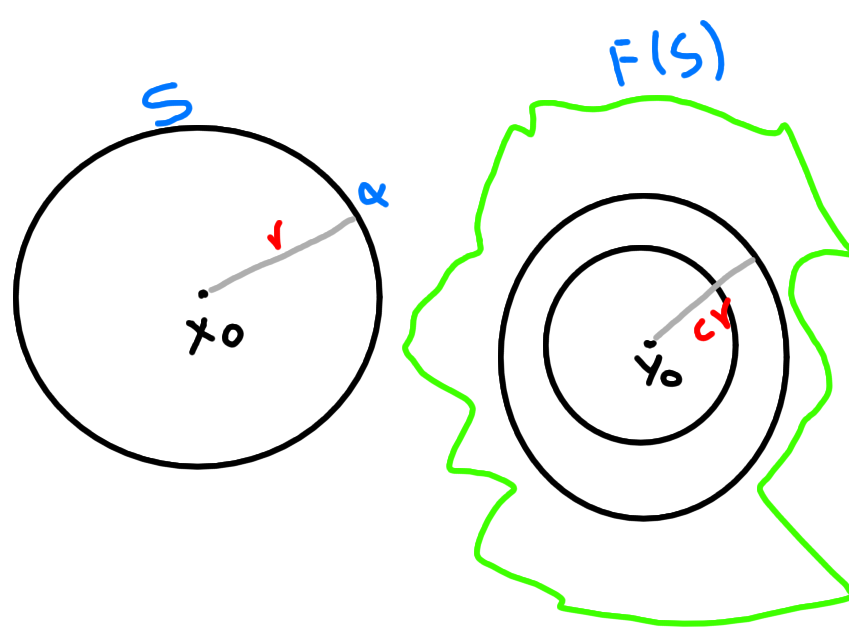
\includegraphics[height=5cm]{fig3.png}
    \caption{stuf}
    \label{fig:fig3}
\end{figure}

Let $x\in S$, eg $\|x-x_0\|=r$. Then we know that \begin{align*}
    \|F(x)-y_0\|&=\|F(x)-F(x_0)\|\geq cr\\
    \|F(x)-y\|&\geq \|F(x)-y_0\|-\|F(x_0)-y_0\|>\frac{cr}{2}
\end{align*}But \begin{align*}
    \|F(x_0)-y\|&=\|y_0-y\|<\frac{cr}{2}
\end{align*}and so $x_0\in B_r(x_0)$, so there's no point in $S$ which can be a minimizer, thus the minimizer must be in the interior of $B_r(x_0)$.

Thus: $\exists U$ nbhd of $x^{*}$ such that \begin{itemize}
    \item $DF(x)$ is invertible $\fora x\in U$
    \item $\exists c>0$ such that $\|F(x)-F(y)\|\geq c\|x-y\|\fora x,y\in U$
    \item $F(U)=V$ is open
    \item $F^{-1}:V\to U$ is well defined. To show it is $C^1$ we will prove \begin{align*}
        F(x)=y\txt{exists and equals}(DF^{-1})(y)=(DF(x))^{-1}
    \end{align*} It suffices to show that \begin{align*}
        \lim_{k\to 0}\frac{\|F^{-1}(y+k)-F^{-1}(y)-[DF(x)]^{-1}k\|}{\|k\|}=0
    \end{align*}
    Notation: $F(x)=y, F(x+h)=y+k$. Then \begin{align*}
        LHS&=\frac{\|h-[DF(x)]^{-1}[F(x+h)-F(x)]}{\|k\|}\\
        &=\frac{\|(DF(x))^{-1}[[DF(x)]h-[F(x+h)-F(x)]]\|}{\|k\|}\\
        &\leq \frac{\|DF(x)^{-1}\|\|F(x+h)-F(x)-DF(x)h\|}{\|k\|}\\
    \end{align*}
    We would like to show that $\|k\|\geq C\|h\|$. We know that $\|F(x+h)-F(x)\|=k\geq c\|h\|$. Then we know that the above limit goes to 0 as $k\to 0$ (since $k\to 0\implies h\to 0$)
\end{itemize}

\underline{Remark:} Another proof of inverse thing: Let $F:\rr^n\to \rr^n, C^1, x^{*}\in \rr^n, DF(x^{*})$ invertible. We will show that $\exists \delta_0>0$ such that if $\|F(x^{*})-y\|<\delta_0$ (divided by some stuff), then $\exists! x\in \bar{B_{\delta_0}}(x^{*})$ such that $F(x)=y$. 

\textbf{Proof:} \begin{align*}
    F(x)=y&\iff x=x-(DF(x^{*}))^{-1}[F(x)-y]
\end{align*}

Note that $x$ is obtained as a fixed point as a fixed point of $T$, \begin{align*}
    x_{k+1}=T(x_k),\{x_k\}\to x\\ 
    x_{k+1}=x_k-(DF(x^{*}))^{-1}[F(x_k)-y]
\end{align*} This looks like Newton's method.

*diagram here that I can't draw because I don't have my tablet*

The main step: To show that $\exists \delta_0$. Then \begin{align*}
    \|x-z-(DF(x^{*}))^{-1}(F(x)-F(z))\|&\leq \frac{1}{2}\|x-z\|\fora x,z\in \bar{B_{\delta_0}}(x^{*})
\end{align*}The LHS becomes \begin{align*}
    \|(DF(x^{*}))^{-1}(F(x)-F(z)-DF(x^{*}(x-z)))\|&\leq \|DF(x^{*})^{-1}\|\|F(x)-F(z)-DF(x^{*}(x-z))\|\\
    &=\|DF(x^{*})^{-1}\|\|\begin{bmatrix}
        \nabla F_1(P_1)\\
        \vdots\\
        \nabla F_n(P_n)
    \end{bmatrix}-DF(x^{*})(x-z)\|
\end{align*} by the MVT.

Choose $\delta_0>0$ such that the above is less than $\frac{1}{2}$. Then the LHS is $\leq \frac{1}{2}\|x-z\|$. Then $T$ is a contraction, and so $T$ has a unique fixed point.

Next we will show that $T:\bar{B_{\delta_0}}(x^{*})\to \bar{B_{\delta_0}}(x^{*})$. Let $\|x-x^{*}\|\leq \delta_0$. Then \begin{align*}
    \|T(x)-x^{*}\|&=\|x-x^{*}-(DF)(x^{*})^{-1}(F(x)-F(x^{*})+F(x^{*})-y)\|\\
    &\leq \|x-x^{*}-DF(x^{*})^{-1}(F(x)-F(x^{*}))\|+\|DF(x^{*})^{-1}\|\|F(x^{*})-y\|\\
    &\leq \frac{1}{2}\|x-x^{*}\|+\frac{1}{2}\delta_0
\end{align*} so $T$ maps $\bar{B_{\delta_0}}(x^{*})$ into $\bar{B_{\delta_0}}(x^{*})$. Then $T$ has a unique fixed point in $\bar{B_{\delta_0}}(x^{*})$, and this fixed point is in $B_{\delta_0}(x^{*})$.

\underline{Remark:} 16.3 \#11 problem: Let $F:\rr^n\to \rr^n, C^1, \exists c\txt{s.t.}\|F(x)-F(y)\|\geq c\|x-y\|$

c.) To show $F(\rr^n)$ is closed, we need $\{y_k\}\subseteq F(\rr^n)$, assume $\{y_k\}\to y\in \rr^n$. We want $y\in F(\rr^n)$. We know that $\exists x_k\in \rr^n, F(x_k)=y_k$. If $\{x_k\}\to x$, then $F(x)=y$. You can show that $\{x_k\}$ is cauchy. Then $\{F(x_k)\}$ is cauchy, and so $F(x_k)\to F(x)$.

\underline{Remark:} Suppose we have $f:\rr^2\to \rr, C^1$. When is $\{(x,y)|f(x,y)=0\}$ a $C^1$ curve? 

A preliminary definition: $C\subseteq \rr^2$ is a $C^1$ curve if $\fora (x_0,y_0)\in C\exists U$ neighborhood of $(x_0, y_0), g:\rr\to\rr, C^1$ such that $C\cap U=\{(x,y)|y=g(x)\}$.

\underline{Fact:} $\fora C\subseteq \rr^2$, closed, $\exists f:\in C^1(\rr^2)$ such that \begin{align*}
    C=\{(x,y)|f(x,y)=0\}
\end{align*}

\underline{Fact:} If $f:\rr^2\to \rr$ is $C^1$, and $\nabla f(x,y)\neq 0\fora (x,y)$ such that $f(x,y)=0$ then $C=\{(x,y)|f(x,y)=0\}$ is a $C^1$ curve.

\textbf{Theorem:} Dim's theorem: Let $O$ open in $\rr^2, f:O\to \rr, C^1$. Let $(x_0,y_0)\in O$, assume $f(x_0,y_0)=0, \partials{f}{y}(x_0,y_0)\neq 0$. Then \begin{align*}
    \exists, r,R>0,g:(x_0-r,x_0+r)\to (y_0-R,y_0+R), C^1\txt{s.t.}f(x,g(x))=0\fora |x-x_0|<r
\end{align*}additionally, if $(x,y)\in (x_0-r,x_0+r)\times (y_0-R,y_0+R)$ and $f(x,y)=0$, then $y=g(x)$.

\textbf{Proof:} $f(x_0,y_0)=0, \partials{f}{y}(x_0,y_0)\neq 0$. WLOG, $\partials{f}{y}(x_0,y_0)>0$. Then \begin{align*}
    \exists R>0, c>0\txt{s.t.}\partials{f}{y}(x,y)>c\fora (x,y)\in [x_0-R,x_0+R]\times [y_0-R,y_0+R]
\end{align*}Since $y\to f(x_0,y)$ is strictly increasing on $[y_0-R, y_0+R]$, $f(x_0,y_0-R)<0, f(x_0, y_0+R)>0$. Also, $\exists r>0$ such that $f(x,y_0-R)<0$ if $|x-x_0|<r, f(x,y_0+R)>0$ if $|x-x_0|<r$. By the IVT for $y\to f(x,y), \fora |x-x_0|<r \exists y\txt{s.t.}f(x,y)=0$. Since $y\to f(x,y)$ is strictly increasing that $y$ is unique. Define $g(x)=y$, the unique y such that $f(x,y)=0, |y-y_0|<R$. We have constructed $g:(x_0-r,x_0+r)\to (y_0-R,y_0+R)$ st $f(x,g(x))=0\fora |x-x_0|<r$ and if $f(x,y)=0$ then $y=g(x)$.

To prove $g\in C^1$ first show $g$ is continuous. Let $x,x+h\in (x_0-r, x_0+r)$. Then \begin{align*}
    f(x+h,g(x+h))-f(x,g(x))&=\iprod{\nabla f(P),(h,g(x+h)-g(x))}\txt{we get $P$ from the MVT}\\
    &=\partials{f}{x}(P)h+\partials{f}{y}(P)(g(x+h)-g(x))\\
    &=0
\end{align*}Then \begin{align*}
    g(x+h)-g(x)&=-\frac{\partials{f}{x}(P)}{\partials{f}{y}(P)}h
\end{align*}We know that the top is $\leq c$ and the bottom is $\geq c$, so $g$ is $C^1$ (since $c>0$)

some stuff missed here about the definition of $g'$-it's what you would expect so I didn't write it.

\underline{Remark:} If we change the dimensions of the domain, eg $f:\rr^{n+1}\to \rr$ of class $C^1$, and $f(x_0\in\rr^n,y_0)=0,\partials{f}{y}(x_0,y_0)\neq 0$. By the same proof as above, $\exists r,R>0,g:(x_0-r,x_0+r)\to (y_0-R,y_0+R), C^1$ such that $f(x,g(x))=0\fora |x-x_0|<r$ and if $f(x,y)=0$ then $y=g(x)$.

\textbf{Theorem:} The implicit function theorem: We take the notation that $(x,y)\in \rr^{n+k}$ where $x\in \rr^n, y\in rr^k$. Then let $O$ be the open set in $\rr^{n+k}$, $f:O\to \rr^k, C^1$. Let $(x_0,y_0)\in O$ such that $F(x_0,y_0)=0, D_yF(x_0,y_0)$ is invertible. Then \begin{align*}
    \exists R, r>0, G:B_r(x_0)\to B_R(y_0), C^1\txt{s.t.}F(x,G(x))=0\fora x\in B_r(x_0)
\end{align*}And additionally; if $x\in B_r(x_0), y\in B_R(y_0)$, and $F(x,y)=0$, then $y=G(x)$. Also, $DG(x)$ can be computed by the chain rule. 

Note that if $k=1$, then we just have the previous theorem.

\textbf{Proof:} Let $H:O\to \rr^{n+k}, H(x,y)=(x,F(x,y))$. Note that $y\in \rr^k, x\in \rr^n$, so $F(x,y)\in \rr^k$. Then, \begin{align*}
    H(x_0,y_0)=(x_0,0)
\end{align*}and the following has a nonzero determinant:

\begin{figure}[H]
    \centering
    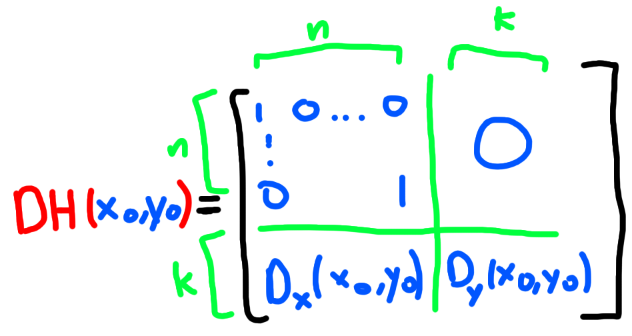
\includegraphics[height=5cm]{fig4.png}
    \caption{eg $DH(x_0,y_0)=\begin{bmatrix}
        I & 0\\
        D_x(x_0,y_0) & D_y(x_0,y_0)
    \end{bmatrix}$}
    \label{fig:fig4}
\end{figure}

Thus the inverse function theorem applies. Then $\exists R>0$ and $V$ neighborhood of $(x_0,0)$ such that $H:B_R(x_0)\times B_R(y_0)\to V$ is 1-1, onto, with a $C^1$ inverse $H^{-1}:V\to \rr^{n+k}, H^{-1}(x,y)=(M(x,y),N(x,y))$.

\begin{figure}[H]
    \centering
    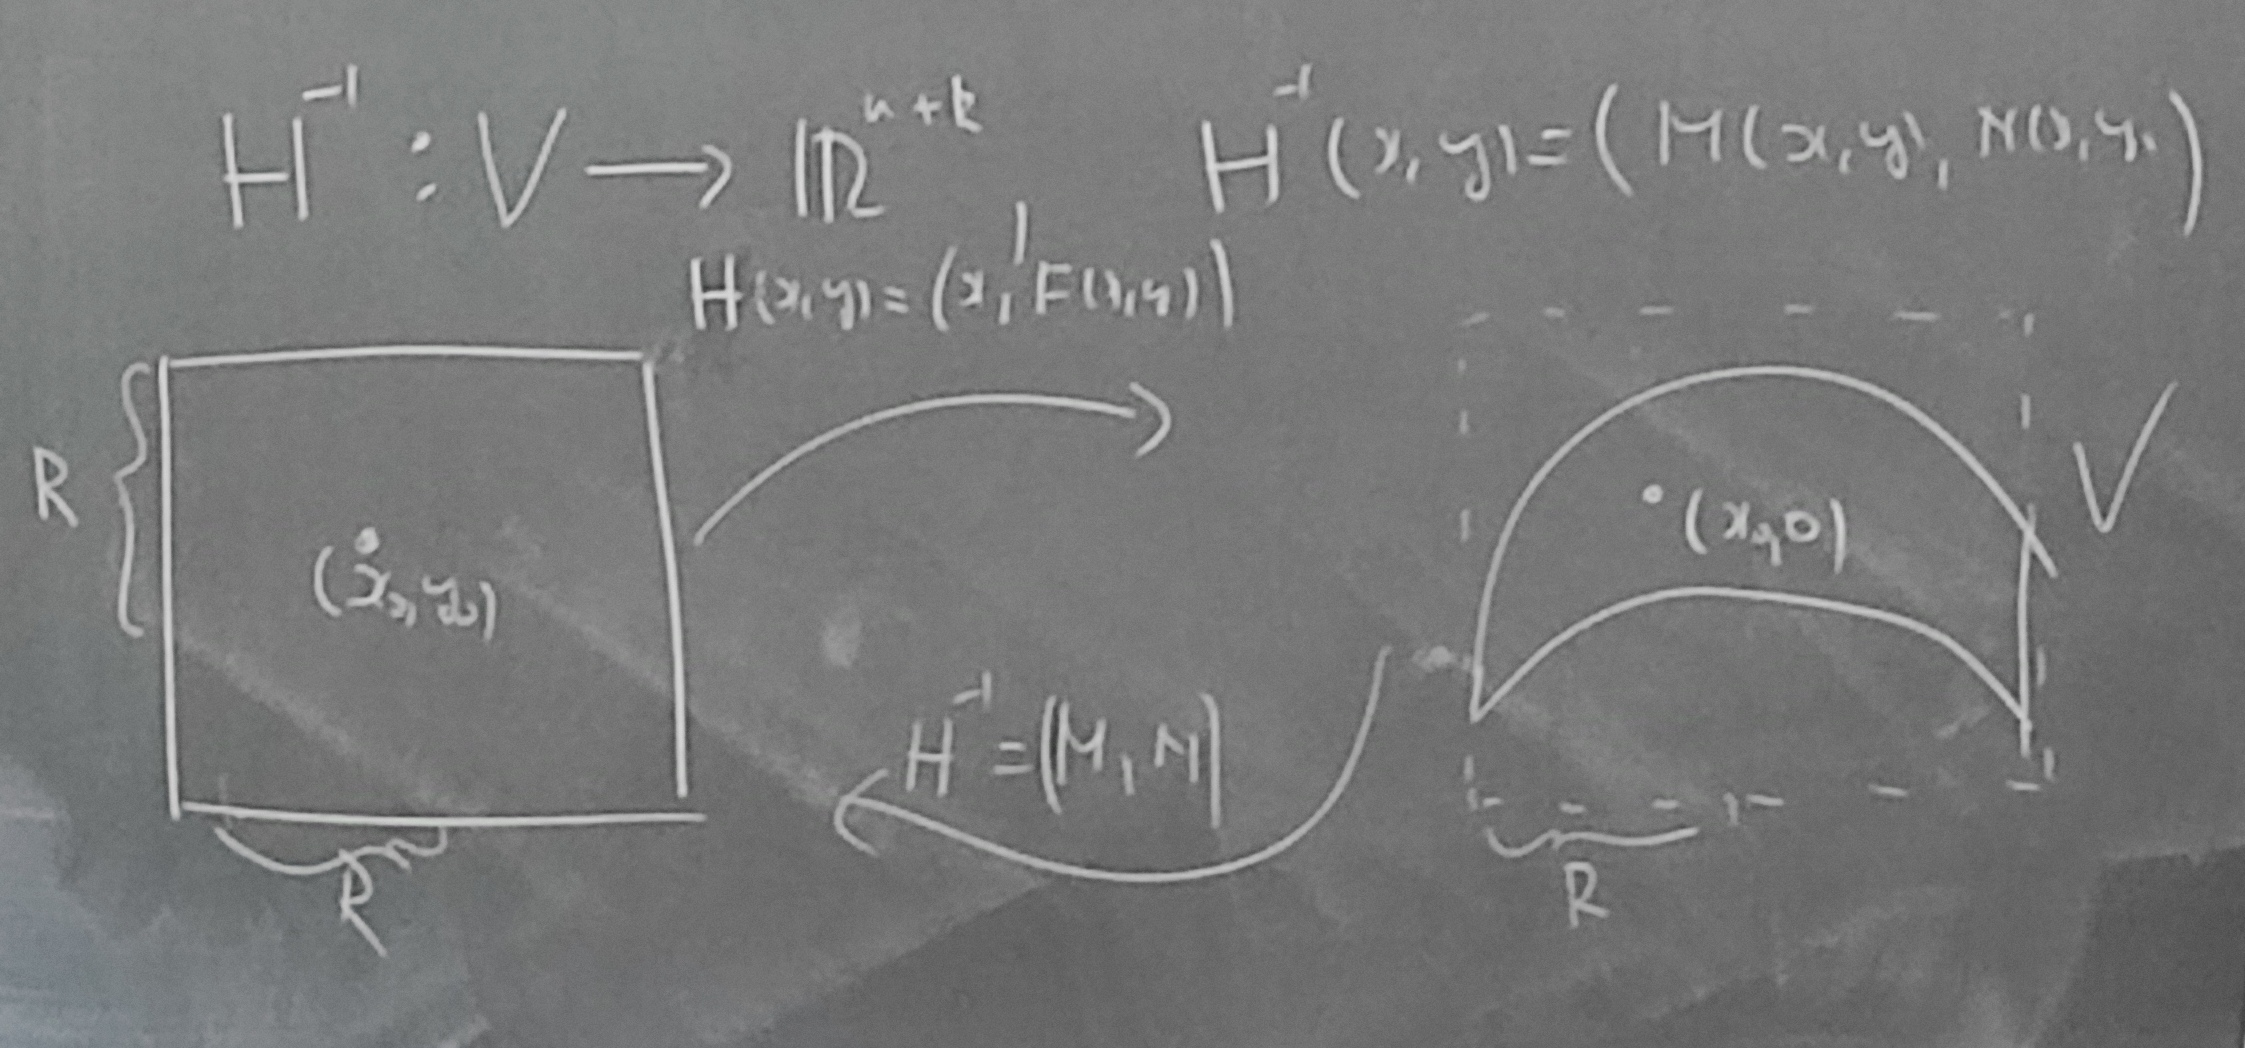
\includegraphics[height=5cm]{fig5.png}
    \caption{"draw a picture" he said}
    \label{fig:fig5}
\end{figure}

Use $H(M(x,y),N(x,y))=(x,y)\fora (x,y)\in V, (M(x,y),F(M(x,y),N(x,y)))=(x,y)$, i.e. $(x,F(x,N(x,y)))=(x,y)$. Then $G(x)=N(x,0)$ is the desired function. Pick $0<r<R$ such that $B_r(x_0)\times \{0\}\subseteq V$. Notice that $G\in C^1$ and that if $x\in B_r(x_0), y\in B_R(y_0)$, and $F(x,y)=0$, then we can write $H^{-1}H(x,y)=0$. Then \begin{align*}
    (M(x,F(x,y)),N(x,F(x,y)))=(x,y)
\end{align*}If $F(x,y)=0$, then $N(x,F(x,y))=y$, so $y=G(x)$.

Finally, we will write down a formula for $DG(x)$ where $x\in B_r(x_0)$. We use a defining property that $F(x,G(x))=0$. Note that a comma denotes a column vector joining; eg \begin{align*}
    x\to (x,G(x))=\begin{bmatrix}
        x\\
        G(x)
    \end{bmatrix}\to F(x,G(x))=0
\end{align*}Then \begin{align*}
    (D_xF(x,G(x)),D_yF(x,G(x)))\begin{bmatrix}
        I\\
        DG(x)
    \end{bmatrix}&=0\\
    (D_xF)(x,G(x))+D_yF(x,G(x))DG(x)&=0\\
\end{align*}$D_y(x,G(x))$ is invertible in a neighborhood of $(x_0,y_0)$, so we can solve for $DG(x)$. Then \begin{align*}
    DG(x)=-(D_yF(x,G(x)))^{-1}D_xF(x,G(x))
\end{align*}

\underline{Example:} Describe a solution for \begin{align*}
    \begin{cases}
        (x^2+y^2+z^2)^3-x+z=0\\
        \cos(x^2+y^2)+e^z-2=0
    \end{cases}
\end{align*}The LHS: $F(x,y,z), F:\rr^3\to \rr^2, F(0,0)=0$. We then expect the function to be a curve through $(0,0,0)\in \rr^3$. \begin{align*}
    DF(0)=\begin{bmatrix}
        -1 & 0 & 1\\
        0 & 0 & 
    \end{bmatrix}
\end{align*}Then we have that \begin{align*}
    y&=(x,z)\\
    x&=y\\
    F(x,G(x))&=0\\
    F(y,G(y))&=0, G:\rr\to \rr^2
\end{align*}
The solutions will then look like $(g_1(y),y,g_2(y))$. 

\section{Chapter 17}

Let $f:\rr^3\to \rr, C^1$. Then let $S=\{(x,y,z)|f(x,y,z)=0\}$, assume $\nabla f(x,y,z)\neq 0 \fora x,y,z\in S$. Then $S$ is a $C^1$ surface. (Recall a definition for $S\subseteq \rr^3$ to be a surface:)\begin{align*}
    \fora x\in S\exists W\txt{nbhd of}x\txt{s.t.}W\cap S=\{(x,y(x))|y(x)\in \rr^2\}
\end{align*}

\textbf{Proof:} Let $(x_0,y_0,z_0)\in S$. WLOG, $\partials{f}{z}(x_0,y_0,z_0)\neq 0$. By the implicit function theorem $\exists r, R>0, g:B_r(x_0)\to B_R(y_0), C^1$ such that $f(x,y,g(x,y))=0\fora x,y\in B_r(x_0)$, and these are the only solutions for $f(x,y,z)=0$ in $B_r(x_0,y_0)\times (z_0-R,z_0+R)$. 

\underline{Theorem:} $(x,y)\to (x,y,g(x,y))$ parameterize $S$ near $(x_0,y_0,z_0)$. Let the tangent vectors at $(x_0,y_0,z_0)$: \begin{align*}
    T_1:(1,0,\partials{g}{x}(x_0,y_0))\\
    T_2:(0,1,\partials{g}{y}(x_0,y_0))
\end{align*}for $x\to (x,y_0,g(x,y_0))$. Then we claim $\nabla f(x_0,y_0,z_0)\perp T_1, T_2$. 

\textbf{Proof:} We want to show the dot product is 0. Look at $f(x,y,g(x,y))=0\fora (x,y)\in B_r(x_0,y_0)$. Then \begin{align*}
    0&=\partials{}{x}|_{x=x_0}f(x,y_0,g(x,y_0))\\
    &=\partials{f}{x}(x_0,y_0,z_0)+\partials{f}{z}(x_0,y_0,z_0)\partials{g}{x}(x_0,y_0)\\
    &=0
\end{align*}Thus $\nabla f(x_0,y_0,z_0)\perp T_1, T_2$. Thus $\exists \lambda\neq 0$ such that $\nabla f(x_0,y_0,z_0)=\lambda(T_1\times T_2)$. Then $S$ is a $C^1$ surface.

\underline{Remark:} Curves in $\rr^3$ defined by the intersection of 2 surfaces: Let $g,h:\rr^3\to \rr,C^1$. Let $C=\{(x,y,z)|g(x,y,z)=h(x,y,z)=0\}$. A sufficient condition for $C$ to be a 1 dimensional curve in $\rr^3$ is $\nabla g(x_0,y_0,z_0)\times \nabla h(x_0,y_0,z_0)\neq 0$.

Equivalently, let $G:\rr^3\to \rr^2, G(x,y,z)=(g(x,y,z),h(x,y,z))$. We require that \begin{align*}
    DG(x_0,y_0,z_0)=\begin{bmatrix}
        \nabla g(x_0,y_0,z_0)\\
        \nabla h(x_0,y_0,z_0)
    \end{bmatrix}
\end{align*}has rank 2 $\fora (x_0,y_0,z_0)\in C$. If so, WLOG, $D_{y,z}G(x_0,y_0,z_0)$ is invertible. Then by the implicit function theorem, $\exists r,R>0, \gamma:B_r(x_0)\to B_R(y_0), C^1$ such that $G(x,\gamma(x))=0\fora |x-x_0|<r$, a unique solution. Then $C$ agrees with the curve $(x,\gamma(x))$.

Parameterize $C: x\to (x,\gamma(x))$. Take the tangent vector at $(x_0,y_0,z_0): (1,\gamma'(x_0))$. Then the cross product of the gradients is a nonzero tangent vector, so $\exists \lambda\neq 0$ such that $\nabla g(x_0,y_0,z_0)\times \nabla h(x_0,y_0,z_0)=\lambda(1,\gamma'(x_0))$.

A generalization: For an $n$ dimensional manifold embedded in $\rr^N,N=n+k$, we have $F:\rr^{n+k}\to \rr^k, C^1$. Assume \begin{align*}
    DF(x_0)=\begin{bmatrix}
        \nabla F_1(x_0)\\
        \vdots\\
        \nabla F_k(x_0)
    \end{bmatrix}
\end{align*}has maximal rank $k$. If so, we will represent the level set $M=\{x|F(x)=0\}$ locally as a graph. Let $X=(x_0,y_0)\in M,x_0\in \rr^n, y_0\in \rr^k$. WLOG $D_yF(x_0,y_0)$ is invertible. Thus $\exists r,R>0, G:B_r(x_0)\to B_R(y_0)$ such that $F(x,G(x))=0$, and is the only solution in $B_r(x_0)\times B_R(y_0)$. Thus $M\cap (B_r(x_0)\times B_R(y_0))=\{(x,G(x))\}$. Then $M$ is locally a graph.

$n$ linearly independent tangent vectors at $(x_0,y_0)$:\begin{align*}
    \begin{bmatrix}
        (1,0,\dots\partials{G_1}{x_1})\\
        \vdots\\
        (0,\dots,1,\partials{G_1}{x_n})
    \end{bmatrix}
\end{align*}

The span of these vectors is the tangent space to $M$ at $(x_0,y_0)$. Then $\nabla F(x_0,y_0)\perp$ the tangent space to $M$ at $(x_0,y_0)$. Then the tangent space to $M$ at $(x_0,y_0)$ is $N(DF(x_0))$.

\underline{Remark:} Suppose you have the function $F:\rr^2\to \rr^3, C^1$.  We have $O\subseteq \rr^2$, open, what is $F(O)$? If $\partials{F}{x}(x,y)\times \partials{F}{y}(x,y)\neq 0\fora (x,y)\in O$, then $F(O)$ is a $C^1$ (smooth) surface. 

Generalize: $F:O\subseteq \rr^k$, open, $\to \rr^N, C^1$. Assume $DF(x_0)$ has some rank $k, N\geq k$. Denote $F=(F_1\in \rr^k, F_2\in \rr^{N-k})$. WLOG, $DF_1(x_0)$ is invertible. Then $\exists U$ neighborhood of $x_0$, $V$ neighborhood of $F_1(x_0)$, st $F(U)=\{(y,G(y))|y\in V\}$ for some $G:V\to \rr^{N-k}, C^1$. Machedon writes $\rr^n$ here but that isn't defined; he must have $N-k=n$.

\textbf{Proof:} $DF_1(x_0)$ is invertible. By the inverse function theorem $\exists U$ a nbhd of $x_0, V$ nbhd of $F_1(x_0)$ such that $F_1:U\to V$ is 1-1, onto, with a $C^1$ inverse $F_1^{-1}:V\to U$. Denote points in $U$ by $x$ and $y$ in $V$. We have that $F(x)=(F_1(x),F_2(x))=(F_1(F_1^{-1}(y)),F_2(F_1^{-1}(y)))=(y,G(y))$.

\underline{Example:} Problem 28; Suppose we have $F:\rr^3\to \rr^2, C^1, F(0,0,0)=(0,0),DF(0,0,0)=\begin{bmatrix}
    0 & 0 & 1\\
    1 & 0 & 0
\end{bmatrix}$, $\exists g,h\in C^1, g,h:(-r,r)\to \rr, g(0)=h(0)=0$ such that \begin{itemize}
    \item $F(x,g(x),h(x))=(0,0)\fora |x|<r$
    \item $F(g(y),y,h(y))=(0,0)\fora |y|<r$
    \item $F(g(z),h(z),z)=(0,0)\fora |z|<r$
\end{itemize}Which of these holds for sure? The second one, since in the implicit function theorem we have that $D_yF(0,0,0)$ is invertible. The free variable is $y$.

*could* the others hold? Is it possible for the first to hold? No. We can't use the implicit function theorem because all that provided us is that the second is true. The problem is the partial derivative with respect to $x$. Assume by contradiction that the first holds. Then \begin{align*}
    DF(0,0,0)\cdot\begin{bmatrix}
        1\\
        g'(0)\\
        h'(0)
    \end{bmatrix}=\begin{bmatrix}
        0\\
        0
    \end{bmatrix}
\end{align*} Why is this a contradiction? Because the second row is $(1,0,0)$ so you pull a nonzero term. 

\underline{Example:} Problem 41; Suppose $F:\rr^2\to \rr^2, C^1, DF(x)$ is positive definite $\fora x\in \rr^2$. Prove that $F$ is 1-1.

\underline{Recall:} $\exists F:\rr^2\to \rr^2, C^1, DF(x)$ invertible $\fora x\in \rr^2$. Then $F$ is 1-1.

\textbf{Proof:} Assume $F(x)=F(x+h), x\in \rr^2$. We must show that $h=0$. We have that \begin{align*}
    F(x+h)-F(x)&=\begin{bmatrix}
        \nabla F_1(P_1)\\
        \nabla F_2(P_2)
    \end{bmatrix}h
\end{align*}Look at $F(x+th)$. We want to write a function that is $\rr\to\rr$ so that we can use the 1 dimensional MVT in order to keep $P_1=P_2$. Consider $\phi(t)=\iprod{F(x+th),h}$. Then $\phi(1)-\phi(0)=\phi'(\theta)$ for some $\theta$ in $(0,1)$. Then \begin{align*}
    \phi(t)&=\iprod{F(x+th),h}\\
    &=\iprod{DF(x+th)h,h}
\end{align*} We are done because we assumed that $\phi(1)-\phi(0)=0$, and so $\iprod{DF(x+\theta h)h,h}>0$ unless $h=0$. 

\underline{Example:} Let $F:\rr^n\to \rr^n, C^1$. Assume $DF(x)$ is invertible, and symmetric. Does $F$ have to be 1-1? 

\underline{Question:} Does there exist $F:\rr^n\to \rr^n, C^1, DF(x)$ invertible $\fora x\in \rr^n, F(\rr^n)$ compact? 

If a function has all points invertible, then by the inverse function theorem, the image is open. Then it can't be compact. 

\subsection{Lagrange Multipliers}

\underline{Case 1:} Surfaces in $\rr^3$. Let $X=(x,y,z)\in \rr^3$, let $g:\rr^3\to \rr, C^1$. Let $S=\{(x,y,z)|g(x,y,z)=0\}$. Assume $\nabla g(x)\neq 0$ if $g(x)=0$. Let $f:\rr^3\to \rr, C^1, x_0\txt{s.t.}f(x_0)\leq f(x)\fora x\in S$ or $f(x_0)\geq f(x)\fora x\in S$. Then $\exists \lambda\in \rr$ such that \begin{align*}
    \nabla f(x_0)=\lambda\nabla g(x_0)
\end{align*}This is the Lagrange multiplier.

\textbf{Proof:} WLOG $\partials{g}{z}(x_0,y_0,z_0)\neq 0$. By the implicit function theorem $\exists h:B_r(x_0,y_0)\to \rr\txt{s.t.}\{x,y,h(x,y)\}$ agrees with $S$ in a neighborhood of $X_0$. Then look at $\phi:B_r(x_0,y_0)\to \rr, \phi(x,y)=f(x,y,h(x,y))=f(H)$ for the purposes of the chain rule; has an unconstrained (internal) minimum or maximum at $(x_0,y_0)$, then $\nabla \phi (x_0,y_0)=0$. By the chain rule \begin{align*}
    \nabla \phi(x_0,y_0)&=\nabla f(x_0,y_0,h(x_0,y_0))DH(x_0,y_0)\\
    &=\nabla f(X_0)\begin{bmatrix}
        1 & 0 \\
        0 & 1 \\
        \partials{h}{x}(x_0,y_0) & \partials{h}{y}(x_0,y_0)
    \end{bmatrix}
\end{align*}The column vectors are the tangent vectors to the surface at $(x_0,y_0)$. Thus $\nabla f(X_0)\perp T_1, T_2$. We know $\nabla g(X_0)\neq 0$ is also normal to $S$. Then $\nabla f(X_0)$ is a scalar multiple of $\nabla g(X_0)$. We call that scalar $\lambda$.

\underline{Remark:} The same argument can be used for the case of $g:\rr^n\to \rr, C^1, M=\{X|g(X)=0\}$, assuming $\nabla g(X)\neq 0$ if $g(X)=0$. Then $f:\rr^n\to \rr, C^1, x_0\in M$ such that $f(x_0)\leq f(x)\fora x\in M$ or $f(x_0)\geq f(x)\fora x\in M$. Then $\exists \lambda\in \rr^n$ such that $\nabla f(x_0)=\lambda\nabla g(x_0)$.

\textbf{Theorem:} $\exists \lambda_1, \lambda_2\in \rr$ such that \begin{align*}
    \nabla f(X_0)=\lambda_1\nabla g_1(X_0)+\lambda_2\nabla g_2(X_0)
\end{align*}

\textbf{Proof:} WLOG, $D_{y,z}(g,h)(x_0,y_0,z_0)$ is invertible. By the implicit function theorem $\exists \gamma:(x_0-r,x_0+r)\to \rr^2, C^1, (x,\gamma(x))$ agrees with $C$ in a neighborhood of $X_0$. Let $\phi(x)=f(x,\gamma(x)), \phi:(x_0-r,x_0+r)\to \rr$. Then $\phi$ has an unconstrained minimum (or maximum) at $x_0$, $\phi'(x_0)=0$. By the chain rule, \begin{align*}
    \nabla f(x_0,\gamma(x_0))\begin{bmatrix}
        1\\
        \gamma'(x_0)
    \end{bmatrix}=0
\end{align*}Recall that $\nabla g(x_0),\nabla h(x_0)$ are linearly independent. Then the vectors are orthogonal to $T$ where $T$ was the matrix above. Then span of $(\nabla g(x_0), \nabla h(x_0))$ is the span of $T$ and so $\nabla f(x_0,\gamma(x_0))$ is a linear combination of $\nabla g(x_0), \nabla h(x_0)$.

\underline{Application:} (don't tell Adam) Let $A$ be an $n\times n$ symmetric real matrix. Let $\lambda=\min_{\|x\|=1}\iprod{Ax,x}$. Then $\lambda$ is an eigenvalue of $A$.

\textbf{Proof:} $g(x)=\|x\|^2, f(x)=\iprod{Ax,x}$ At a minimizer, $\nabla f(x_0)=\lambda x_0$. Then $\exists \lambda\in \rr$ such that $\nabla f(x_0)=\lambda\nabla g(x_0)$.

\underline{Lemma:} If $f(x)=\iprod{Ax, x}$, then $\nabla f(x)=2Ax$.

\textbf{Proof:} \begin{align*}
    \lim_{t\to 0}\frac{f(x+te_i)-f(x)}{t}&=\lim_{t\to 0}\frac{\iprod{A(x+te_i),x+te_i}-\iprod{Ax,x}}{t}\\
    &=\lim_{t\to 0}\frac{t\iprod{Ax, e_i}+t\iprod{Ae_i,x}+t^2\iprod{Ae_i,e_i}}{t}\\
    &=\iprod{Ax,e_i}+\iprod{Ae_i,x}\\
    &=2\iprod{Ax,e_i}
\end{align*}

\underline{Problem:} Let $p>1, q>1$. Prove \begin{align*}
    \frac{x^p}{p}+\frac{y^q}{q}\geq \frac{1}{p}+\frac{1}{q}
\end{align*}If $g(x,y)=xy=1, x>0, y>0$. At a minimizer $\nabla f=\lambda\nabla g, xy=1$. Then \begin{align*}
    \begin{cases}
        x^{p-1}=\lambda y\\
        y^{g-1}=\lambda x\\
        xy = 1
    \end{cases}
\end{align*}Then \begin{align*}
    \begin{cases}
        \lambda=\frac{x^{p-1}}{y}=\frac{y^{g-1}}{x}\\
        xy = 1
    \end{cases}
\end{align*}

My computer is running out of battery. I probably can't tex notes for the rest of this class, but I will list the topics we went over here:\begin{itemize}
    \item See discord DMS for a scan of the handwritten notes 
\end{itemize}

\underline{Remark:} Suppose $R$ is a rectangle in $\rr^2$, bounded on x by $[a,b]$ and on y by $[c,d]$.

Let $P_1=\{a=x_1<\dots<x_n=b\}$ be a partition of $[a,b]$. Let $P_2=\{c=y_1<\dots<y_l=d\}$ be a partition of $[c,d]$. Let Let $P=\{[x_{i-1},x_i]\times [y_{j-1},y_j]\}$ be a partition of $R$. Let $f:R\to \rr$, bounded. 

For some $J\in P$, let $m(f, J)=\inf_{(x,y)\in J}f, M(f,J)=\sup_{(x,y)\in J}f$. Then \begin{align*}
    L(f,P)=\sum_{J\in P}m(f,J)\Delta J, U(f,P)=\sum_{J\in P}M(f,J)\Delta J
\end{align*}where $\Delta J$ is the area of $J$. Then \begin{align*}
    \underline{\int}f = \sup_{P}L(f,P), \overline{\int}f=\inf_{P}U(f,P)
\end{align*}

\textbf{Definition:} $f$ is Riemann integrable on $R$ if \begin{align*}
    \underline{\int}f=\overline{\int}f=\int_R f
\end{align*}

\underline{Remark:} Let $D\subseteq \rr^2$, bounded. To define $\int_D f$, choose $R$ a rectangle so that $D\subseteq R$. Extend $f$ to $\tilde{f}$, such that \begin{align*}
    \tilde{f}(x,y)=\begin{cases}
        f(x,y) & (x,y)\in D\\
        0 & (x,y)\in R\setminus D
    \end{cases}
\end{align*}Define $\int_D f=\int_R \tilde{f}$.

\textbf{Definition:} Let $S\subseteq \rr^n$. Then $S$ has Jordan content 0 if $\fora \epsilon>0, \exists \{R_i\}$ a collection of rectangles such that $S\subseteq \bigcup R_i$ and $\sum \text{vol}(R_i)<\epsilon$. Note that $i$ finite. 

\textbf{Theorem:} Let $f:R\to \rr$, bounded. If the set of points where $f$ is discontinuous has Jordan content 0, then $f$ is Riemann integrable.

\textbf{Definition:} A set $S\subseteq \rr^n$ has Lebesgue measure 0 if $\fora \epsilon>0, \exists \{Q_i\}$, all open, countably many (not finitely many), a collection of rectangles such that $S\subseteq \bigcup Q_i$ and $\sum \text{vol}(Q_i)<\epsilon$.

\textbf{Theorem:} Let $f:R\to \rr$, bounded. $f$ is Riemann integrable iff. the set of points where $f$ is discontinuous has Lebesgue measure 0.

\underline{Example:} $Q\bigcap [0,1]$ has Jordan content 0? No. It's countable but the sum of the lengths greater or equal to 1. 

How about Lebesgue measure 0? Yes, use intervals $(r_k-\frac{\epsilon}{2^i},r_k+\frac{\epsilon}{2^i})$.

\underline{Corollary:} If $f:[0,1]\to \rr$ is discontinuous, at all rational points, and continuous at all irrational points, then $f$ is Riemann integrable.

One such function is the function, $f(x)=\begin{cases}
    0 & x\notin \mathbb{Q}\\
    1/q & x=p/q \in \mathbb{Q}, q>0
\end{cases}$. Have fun convincing yourself this is continuous on the irrationals - consider arbitrarily large q to do so.

\textbf{Skipped this lecture!}

\underline{Recall:} If $\phi: O\to \phi(O)$ is 1-1, $C^1$, and rank $D\phi(x)=k\fora x\in O$, define \begin{align*}
    g_{ij}(x)=\iprod{\partials{\phi}{x_i}(x),\partials{\phi}{x_j}(x)}\\
    (g_{ij}(x))=(D\phi(x))^T(D\phi(x))
\end{align*}

\textbf{Definition:} Let $f$ continuous on $M$. Then \begin{align*}
    \int_{\phi(O)}f dS = \int_O f(\phi(x))\sqrt{\det(g_{ij}(x))}dx
\end{align*}

\underline{Example:} Let $k=n, \phi:U\subseteq\rr^n\to V\subseteq \rr^n$, 1-1, onto, $D\phi(x)$ invertible. Then $D(\phi(x))$ is an $n\times n$ matrix, $\det(g_{ij}(x))=\det(D\phi(x))^T(D\phi(x))=\det(D\phi(x))^2$. Then \begin{align*}
    \int_{\phi(U)}f dx = \int_U f(\phi(x))|\det(D\phi(x))|dx
\end{align*} This looks like a change of variables formula.

\underline{Example:} $M\subseteq \rr^n$ is the graph of a $C^1$ function $r:U\subseteq\rr^{n-1}\to \rr$. Then $\phi(x)=(x,r(x))$ is the parametrization, $D\phi(x)=\begin{bmatrix}
    I\\
    \partials{r}{x_1}(x)\\
    \vdots\\
    \partials{r}{x_{n-1}}(x)
\end{bmatrix}$. Then $g_{ij}(x)=[D\phi(x)]^T[D\phi(x)]$ is the identity matrix plus the gradient of $r$ squared. Then \begin{align*}
    \int_M f dS = \int_U f(x,r(x))\sqrt{1+|\nabla r(x)|^2}dx
\end{align*}

\underline{Lemma:} Let $v$ be a column vectors in $\rr^n$. Then \begin{align*}
    \det([I v]\begin{bmatrix}
        I\\v
    \end{bmatrix})=1+|v|^2
\end{align*}

\section{Convolutions}

Let $f,g:\rr\to\rr$, continuous, $g$ compactly supported (to be defined). Look at the set of points such that $\text{supp} g = {x|g(x)\neq 0}$, i.e. $g(x)=0$ for $|x|>R$. Then 

\textbf{Definition:} \begin{align*}
    (f*g)(x)=\int_{-\infty}^{\infty}f(x-y)g(y)dy=\int_{-\infty}^{\infty}f(y)g(x-y)dy=(g*f)(x)
\end{align*}

Fix $g:\rr\to \rr$, continuous, $g$ supported in $(-1,1), \int_{-\infty}^{\infty}g(x)dx=1$. Define \begin{align*}
    g_\delta(x)=\frac{1}{\delta}g(\frac{x}{\delta})
\end{align*}Then $g_\delta$ is supported in $(-\delta,\delta)$ and $\int_{-\infty}^{\infty}g_\delta(x)dx=1$.

\textbf{Theorem:} Let $f:\rr\to\rr$, continuous, $g$ as above. Then \begin{align*}
    \lim_{\delta\to 0+}(f*g_\delta)(x)=f(x)
\end{align*}if $f(x)$ is uniformly continuous, then the convergence is uniform. 

\textbf{Proof:} \begin{align*}
    \int_{-\infty}^{\infty}f(x-y)g_\delta(y)dy-g(x)&=\int_{-\infty}^{\infty}(f(x-y)-f(x))g_\delta(y)dy\\
    &=\int_{-\infty}^{\infty}(f(x-y)-f(x))\frac{1}{\delta}g(\frac{y}{\delta})dy\\
    &=\int_{-\infty}^{\infty}(f(x-\delta y)-f(x))g(y)dy
\end{align*}Take the absolute value of everything. After that, \begin{align*}
    |\int_{-\infty}^{\infty}f(x-y)g_\delta(y)dy-g(x)|&\leq \int_{-\infty}^{\infty}|f(x-\delta y)-f(x)||g(y)|dy\\
    &=\int_{-1}^{1}|f(x-\delta y)-f(x)||g(y)|dy
\end{align*}Let $\epsilon>0$. $\exists \delta>0$ s.t. $|f(x-\delta y)-f(x)|<\epsilon\fora |y|<1$. Then $RHS\leq \epsilon\cdot\int |g(y)|dy=c\epsilon$. If $f$ is uniformly continuous, then the estimate is uniform in $x$.

\textbf{Definition:} $\Omega \subseteq \rr^n$ is an open set with $C^1$ boundary. If $\exists k:\rr^n\to \rr, C^1, \nabla k(x)\neq 0$ if $k(x)=0$ such that $\Omega=\{x\in \rr^n|r(x)>0\}$. 

By the implicit function theorem, if $\Omega$ is an open set with $C^1$ boundary, $\fora x_0\in\txt{boundary}\Omega \exists U\txt{nbhd}x_0, r$ a $C^1$ function of $n-1$ variables such that $\Omega\cap U=\{x_n>r(x_1,\dots,x_{n-1})\}\cap U$. 

\textbf{Theorem:} Let $\Omega\subseteq \rr^n$ be a bounded open set with $C^1$ boundary. Let $f_1,\dots,f_n$ be $C^1$ in a neighborhood of $\overline{\Omega}$. Then \begin{align*}
    \int_{\Omega}\partials{f_1}{x_1}+\dots+\partials{f_n}{x_n}dx=\int_{\partial\Omega}f_1dx_1+\dots+f_ndx_n
\end{align*}

\textbf{Proof:} Equivalent formulation is that \begin{align*}
    \int_{\Omega}\nabla f(x)dx = \int_{\partial\Omega}fNdS\\
\end{align*}Prove this for $f\in C^1$ supported in $\Omega$ 

\underline{Lemma:} If $f\in C_0^1(\Omega)$ where $C_0$ indicates it's compactly supported in $\Omega$, then \begin{align*}
    \int_{\Omega}\partials{f}{x_i}(x)dx&=\int_{\rr^n}\partials{f}{x_i}(x)dx\\
    &=\int_{\rr^{n-1}}\int_{-\infty}^{\infty}\partials{f}{x_i}(x_1,\dots,x_n)dx_ndx_1\dots dx_{n-1}\\
\end{align*}

Then we prove this for $f$ supported in $V$, a neighborhood of a point in $\partial \Omega$ where \begin{align*}
    \Omega\cap V=\{x_n>r(x_1,\dots,x_{n-1})\}\cap V
\end{align*}

Doing that in $\rr^2$; then \begin{align*}
    \Omega\cap V=\{y>r(x)\}\cap V
\end{align*}and $\nabla(r(x)-y)=(r'(x),-1)=\tilde{N}$. We want normal \begin{align*}
    N:\frac{1}{\sqrt{1+r'(x)^2}}(-r'(x),1)
\end{align*}
Then you integrate by parts.If $f,g\in C_0^1(\rr^n)$, then \begin{align*}
    \int_{\rr^n}\partials{f}{x_i}gdx=-\int_{\rr^n}f\partials{g}{x_i}dx
\end{align*}
Recall the Heaviside function \begin{align*}
    H(t)=\begin{cases}
        1 & t>0\\
        0 & t<0
    \end{cases}
\end{align*}, and define \begin{align*}
    h(t)=\begin{cases}
        0 & t\leq 0\\
        1 & t\geq 1
    \end{cases}
\end{align*}Then, \begin{align*}
    \lim_{\delta\to 0}h(\frac{t}{\delta})=H(t)
\end{align*}

Continuing with the proof, \begin{align*}
    \int_{\Omega}(\nabla f)(x,y)dxdy&=\int_{-\infty}^{\infty}(\int_{r(x)}^{\infty}\nabla f(x,y)dy)dx\\
    &=\int_{-\infty}^{\infty}(\int_{-\infty}^{\infty})H(y-r(x)\nabla f(x,y)dy)dx\\
    &=?\lim_{\delta\to 0}\int_{-\infty}^{\infty}(\int_{-\infty}^{\infty}h(\frac{y-r(x)}{\delta})\nabla f(x,y)dy)dx\\
    &=-\lim_{\delta\to 0}\int_{-\infty}^{\infty}\int_{-\infty}^{\infty}\frac{1}{\delta}((-r'(x),1)\cdot(\frac{1}{\delta}h'(\frac{y-r(x)}{\delta}))f(x,y)dy)dx\\
    &=\lim_{\delta\to 0}\int_{-\infty}^{\infty}(\int_{-\infty}^{\infty}\tilde{N}(x)\frac{1}{\delta}h'(\frac{y-r(x)}{\delta})f(x,y)dy)dx\\
    &=?\int_{-\infty}^{\infty}(\lim_{\delta\to 0}\int_{-\infty}^{\infty}\frac{1}{\delta}h'(\frac{y-r(x)}{\delta})f(x,y)\tilde{N}(x)dy)dx\\
    &=\int_{-\infty}^{\infty}(f(x,r(x))\tilde{N}(x))dx\\
    &=\int_{\partial\Omega}fNdS
\end{align*}

There are two equalities that require some justification. They were highlighted with a $?$ in the above proof. Because I was too lazy to explain it, either see the textbook or just trust me bro \texttrademark

\section{Fall 2023 Final Questions}

\textbf{Question:} If $U_1, U_2$ are disjoint nonempty open sets in $\rr^n$, then $\exists c>0$ s.t. $\|x-y\|\geq c \fora x\in U_1, y\in U_2$. True or False?

\textbf{Answer:} False. Consider two open balls right next to each other. Take x,y literally right next to each other. Then $\|x-y\|$ is arbitrarily small.

\textbf{Question:} $f_n(x)=nx^n(1-x), f_n:[0,1]\to \rr$. \begin{itemize}
    \item Find $\lim_{n\to \infty}f_n(x)$ pointwise.
    \item Is this uniform?
\end{itemize}

\textbf{Answer:} \begin{itemize}
    \item $0$
    \item To be seen on Friday \texttrademark
\end{itemize}

\end{document}